\documentclass[a4paper,12pt]{article}
	\usepackage{helvet}
    \renewcommand{\familydefault}{\sfdefault}
	\usepackage{setspace}
	\onehalfspacing
    \usepackage[breakable]{tcolorbox}
    \usepackage{parskip} % Stop auto-indenting (to mimic markdown behaviour)
    \usepackage{tabto}
    \usepackage{iftex}
    \ifPDFTeX
    	\usepackage[T1]{fontenc}
    	\usepackage{mathpazo}
    \else
    	\usepackage{fontspec}
    \fi
	\usepackage[utf8]{inputenc}
    % Basic figure setup, for now with no caption control since it's done
    % automatically by Pandoc (which extracts ![](path) syntax from Markdown).
    \usepackage{graphicx}
    % Maintain compatibility with old templates. Remove in nbconvert 6.0
    \let\Oldincludegraphics\includegraphics
    % Ensure that by default, figures have no caption (until we provide a
    % proper Figure object with a Caption API and a way to capture that
    % in the conversion process).
    \usepackage{caption}
    \DeclareCaptionFormat{nocaption}{}
    \captionsetup{format=nocaption,aboveskip=0pt,belowskip=0pt}

    \usepackage{float}
    \floatplacement{figure}{H} % forces figures to be placed at the correct location
    \usepackage{xcolor} % Allow colors to be defined
    \usepackage{enumerate} % Needed for markdown enumerations to work
    \usepackage{geometry} % Used to adjust the document margins
    \usepackage{amsmath} % Equations
    \usepackage{amssymb} % Equations
    \usepackage{textcomp} % defines textquotesingle
    % Hack from http://tex.stackexchange.com/a/47451/13684:
    \AtBeginDocument{%
        \def\PYZsq{\textquotesingle}% Upright quotes in Pygmentized code
    }
    \usepackage{upquote} % Upright quotes for verbatim code
    \usepackage{eurosym} % defines \euro
    \usepackage[mathletters]{ucs} % Extended unicode (utf-8) support
    \usepackage{fancyvrb} % verbatim replacement that allows latex
    \usepackage{grffile} % extends the file name processing of package graphics 
                         % to support a larger range
    \makeatletter % fix for old versions of grffile with XeLaTeX
    \@ifpackagelater{grffile}{2019/11/01}
    {
      % Do nothing on new versions
    }
    {
      \def\Gread@@xetex#1{%
        \IfFileExists{"\Gin@base".bb}%
        {\Gread@eps{\Gin@base.bb}}%
        {\Gread@@xetex@aux#1}%
      }
    }
    \makeatother
    \usepackage[Export]{adjustbox} % Used to constrain images to a maximum size
    \adjustboxset{max size={0.9\linewidth}{0.9\paperheight}}

    % The hyperref package gives us a pdf with properly built
    % internal navigation ('pdf bookmarks' for the table of contents,
    % internal cross-reference links, web links for URLs, etc.)
    \usepackage{hyperref}
    % The default LaTeX title has an obnoxious amount of whitespace. By default,
    % titling removes some of it. It also provides customization options.
    \usepackage{titling}
    \usepackage{longtable} % longtable support required by pandoc >1.10
    \usepackage{booktabs}  % table support for pandoc > 1.12.2
    \usepackage[inline]{enumitem} % IRkernel/repr support (it uses the enumerate* environment)
    \usepackage[normalem]{ulem} % ulem is needed to support strikethroughs (\sout)
                                % normalem makes italics be italics, not underlines
    \usepackage{mathrsfs}
    

    
    % Colors for the hyperref package
    \definecolor{urlcolor}{rgb}{0,.145,.698}
    \definecolor{linkcolor}{rgb}{.71,0.21,0.01}
    \definecolor{citecolor}{rgb}{.12,.54,.11}

    % ANSI colors
    \definecolor{ansi-black}{HTML}{3E424D}
    \definecolor{ansi-black-intense}{HTML}{282C36}
    \definecolor{ansi-red}{HTML}{E75C58}
    \definecolor{ansi-red-intense}{HTML}{B22B31}
    \definecolor{ansi-green}{HTML}{00A250}
    \definecolor{ansi-green-intense}{HTML}{007427}
    \definecolor{ansi-yellow}{HTML}{DDB62B}
    \definecolor{ansi-yellow-intense}{HTML}{B27D12}
    \definecolor{ansi-blue}{HTML}{208FFB}
    \definecolor{ansi-blue-intense}{HTML}{0065CA}
    \definecolor{ansi-magenta}{HTML}{D160C4}
    \definecolor{ansi-magenta-intense}{HTML}{A03196}
    \definecolor{ansi-cyan}{HTML}{60C6C8}
    \definecolor{ansi-cyan-intense}{HTML}{258F8F}
    \definecolor{ansi-white}{HTML}{C5C1B4}
    \definecolor{ansi-white-intense}{HTML}{A1A6B2}
    \definecolor{ansi-default-inverse-fg}{HTML}{FFFFFF}
    \definecolor{ansi-default-inverse-bg}{HTML}{000000}

    % common color for the border for error outputs.
    \definecolor{outerrorbackground}{HTML}{FFDFDF}

    % commands and environments needed by pandoc snippets
    % extracted from the output of `pandoc -s`
    \providecommand{\tightlist}{%
      \setlength{\itemsep}{0pt}\setlength{\parskip}{0pt}}
    \DefineVerbatimEnvironment{Highlighting}{Verbatim}{commandchars=\\\{\}}
    % Add ',fontsize=\small' for more characters per line
    \newenvironment{Shaded}{}{}
    \newcommand{\KeywordTok}[1]{\textcolor[rgb]{0.00,0.44,0.13}{\textbf{{#1}}}}
    \newcommand{\DataTypeTok}[1]{\textcolor[rgb]{0.56,0.13,0.00}{{#1}}}
    \newcommand{\DecValTok}[1]{\textcolor[rgb]{0.25,0.63,0.44}{{#1}}}
    \newcommand{\BaseNTok}[1]{\textcolor[rgb]{0.25,0.63,0.44}{{#1}}}
    \newcommand{\FloatTok}[1]{\textcolor[rgb]{0.25,0.63,0.44}{{#1}}}
    \newcommand{\CharTok}[1]{\textcolor[rgb]{0.25,0.44,0.63}{{#1}}}
    \newcommand{\StringTok}[1]{\textcolor[rgb]{0.25,0.44,0.63}{{#1}}}
    \newcommand{\CommentTok}[1]{\textcolor[rgb]{0.38,0.63,0.69}{\textit{{#1}}}}
    \newcommand{\OtherTok}[1]{\textcolor[rgb]{0.00,0.44,0.13}{{#1}}}
    \newcommand{\AlertTok}[1]{\textcolor[rgb]{1.00,0.00,0.00}{\textbf{{#1}}}}
    \newcommand{\FunctionTok}[1]{\textcolor[rgb]{0.02,0.16,0.49}{{#1}}}
    \newcommand{\RegionMarkerTok}[1]{{#1}}
    \newcommand{\ErrorTok}[1]{\textcolor[rgb]{1.00,0.00,0.00}{\textbf{{#1}}}}
    \newcommand{\NormalTok}[1]{{#1}}
    
    % Additional commands for more recent versions of Pandoc
    \newcommand{\ConstantTok}[1]{\textcolor[rgb]{0.53,0.00,0.00}{{#1}}}
    \newcommand{\SpecialCharTok}[1]{\textcolor[rgb]{0.25,0.44,0.63}{{#1}}}
    \newcommand{\VerbatimStringTok}[1]{\textcolor[rgb]{0.25,0.44,0.63}{{#1}}}
    \newcommand{\SpecialStringTok}[1]{\textcolor[rgb]{0.73,0.40,0.53}{{#1}}}
    \newcommand{\ImportTok}[1]{{#1}}
    \newcommand{\DocumentationTok}[1]{\textcolor[rgb]{0.73,0.13,0.13}{\textit{{#1}}}}
    \newcommand{\AnnotationTok}[1]{\textcolor[rgb]{0.38,0.63,0.69}{\textbf{\textit{{#1}}}}}
    \newcommand{\CommentVarTok}[1]{\textcolor[rgb]{0.38,0.63,0.69}{\textbf{\textit{{#1}}}}}
    \newcommand{\VariableTok}[1]{\textcolor[rgb]{0.10,0.09,0.49}{{#1}}}
    \newcommand{\ControlFlowTok}[1]{\textcolor[rgb]{0.00,0.44,0.13}{\textbf{{#1}}}}
    \newcommand{\OperatorTok}[1]{\textcolor[rgb]{0.40,0.40,0.40}{{#1}}}
    \newcommand{\BuiltInTok}[1]{{#1}}
    \newcommand{\ExtensionTok}[1]{{#1}}
    \newcommand{\PreprocessorTok}[1]{\textcolor[rgb]{0.74,0.48,0.00}{{#1}}}
    \newcommand{\AttributeTok}[1]{\textcolor[rgb]{0.49,0.56,0.16}{{#1}}}
    \newcommand{\InformationTok}[1]{\textcolor[rgb]{0.38,0.63,0.69}{\textbf{\textit{{#1}}}}}
    \newcommand{\WarningTok}[1]{\textcolor[rgb]{0.38,0.63,0.69}{\textbf{\textit{{#1}}}}}
    
    
    % Define a nice break command that doesn't care if a line doesn't already
    % exist.
    \def\br{\hspace*{\fill} \\* }
    % Math Jax compatibility definitions
    \def\gt{>}
    \def\lt{<}
    \let\Oldtex\TeX
    \let\Oldlatex\LaTeX
    \renewcommand{\TeX}{\textrm{\Oldtex}}
    \renewcommand{\LaTeX}{\textrm{\Oldlatex}}
    % Document parameters
    % Document title
    \title{Entwicklung einer KI für das Schach-Endspiel \\ Studienarbeit} 
    
    
    
    
% Pygments definitions
\makeatletter
\def\PY@reset{\let\PY@it=\relax \let\PY@bf=\relax%
    \let\PY@ul=\relax \let\PY@tc=\relax%
    \let\PY@bc=\relax \let\PY@ff=\relax}
\def\PY@tok#1{\csname PY@tok@#1\endcsname}
\def\PY@toks#1+{\ifx\relax#1\empty\else%
    \PY@tok{#1}\expandafter\PY@toks\fi}
\def\PY@do#1{\PY@bc{\PY@tc{\PY@ul{%
    \PY@it{\PY@bf{\PY@ff{#1}}}}}}}
\def\PY#1#2{\PY@reset\PY@toks#1+\relax+\PY@do{#2}}

\@namedef{PY@tok@w}{\def\PY@tc##1{\textcolor[rgb]{0.73,0.73,0.73}{##1}}}
\@namedef{PY@tok@c}{\let\PY@it=\textit\def\PY@tc##1{\textcolor[rgb]{0.24,0.48,0.48}{##1}}}
\@namedef{PY@tok@cp}{\def\PY@tc##1{\textcolor[rgb]{0.61,0.40,0.00}{##1}}}
\@namedef{PY@tok@k}{\let\PY@bf=\textbf\def\PY@tc##1{\textcolor[rgb]{0.00,0.50,0.00}{##1}}}
\@namedef{PY@tok@kp}{\def\PY@tc##1{\textcolor[rgb]{0.00,0.50,0.00}{##1}}}
\@namedef{PY@tok@kt}{\def\PY@tc##1{\textcolor[rgb]{0.69,0.00,0.25}{##1}}}
\@namedef{PY@tok@o}{\def\PY@tc##1{\textcolor[rgb]{0.40,0.40,0.40}{##1}}}
\@namedef{PY@tok@ow}{\let\PY@bf=\textbf\def\PY@tc##1{\textcolor[rgb]{0.67,0.13,1.00}{##1}}}
\@namedef{PY@tok@nb}{\def\PY@tc##1{\textcolor[rgb]{0.00,0.50,0.00}{##1}}}
\@namedef{PY@tok@nf}{\def\PY@tc##1{\textcolor[rgb]{0.00,0.00,1.00}{##1}}}
\@namedef{PY@tok@nc}{\let\PY@bf=\textbf\def\PY@tc##1{\textcolor[rgb]{0.00,0.00,1.00}{##1}}}
\@namedef{PY@tok@nn}{\let\PY@bf=\textbf\def\PY@tc##1{\textcolor[rgb]{0.00,0.00,1.00}{##1}}}
\@namedef{PY@tok@ne}{\let\PY@bf=\textbf\def\PY@tc##1{\textcolor[rgb]{0.80,0.25,0.22}{##1}}}
\@namedef{PY@tok@nv}{\def\PY@tc##1{\textcolor[rgb]{0.10,0.09,0.49}{##1}}}
\@namedef{PY@tok@no}{\def\PY@tc##1{\textcolor[rgb]{0.53,0.00,0.00}{##1}}}
\@namedef{PY@tok@nl}{\def\PY@tc##1{\textcolor[rgb]{0.46,0.46,0.00}{##1}}}
\@namedef{PY@tok@ni}{\let\PY@bf=\textbf\def\PY@tc##1{\textcolor[rgb]{0.44,0.44,0.44}{##1}}}
\@namedef{PY@tok@na}{\def\PY@tc##1{\textcolor[rgb]{0.41,0.47,0.13}{##1}}}
\@namedef{PY@tok@nt}{\let\PY@bf=\textbf\def\PY@tc##1{\textcolor[rgb]{0.00,0.50,0.00}{##1}}}
\@namedef{PY@tok@nd}{\def\PY@tc##1{\textcolor[rgb]{0.67,0.13,1.00}{##1}}}
\@namedef{PY@tok@s}{\def\PY@tc##1{\textcolor[rgb]{0.73,0.13,0.13}{##1}}}
\@namedef{PY@tok@sd}{\let\PY@it=\textit\def\PY@tc##1{\textcolor[rgb]{0.73,0.13,0.13}{##1}}}
\@namedef{PY@tok@si}{\let\PY@bf=\textbf\def\PY@tc##1{\textcolor[rgb]{0.64,0.35,0.47}{##1}}}
\@namedef{PY@tok@se}{\let\PY@bf=\textbf\def\PY@tc##1{\textcolor[rgb]{0.67,0.36,0.12}{##1}}}
\@namedef{PY@tok@sr}{\def\PY@tc##1{\textcolor[rgb]{0.64,0.35,0.47}{##1}}}
\@namedef{PY@tok@ss}{\def\PY@tc##1{\textcolor[rgb]{0.10,0.09,0.49}{##1}}}
\@namedef{PY@tok@sx}{\def\PY@tc##1{\textcolor[rgb]{0.00,0.50,0.00}{##1}}}
\@namedef{PY@tok@m}{\def\PY@tc##1{\textcolor[rgb]{0.40,0.40,0.40}{##1}}}
\@namedef{PY@tok@gh}{\let\PY@bf=\textbf\def\PY@tc##1{\textcolor[rgb]{0.00,0.00,0.50}{##1}}}
\@namedef{PY@tok@gu}{\let\PY@bf=\textbf\def\PY@tc##1{\textcolor[rgb]{0.50,0.00,0.50}{##1}}}
\@namedef{PY@tok@gd}{\def\PY@tc##1{\textcolor[rgb]{0.63,0.00,0.00}{##1}}}
\@namedef{PY@tok@gi}{\def\PY@tc##1{\textcolor[rgb]{0.00,0.52,0.00}{##1}}}
\@namedef{PY@tok@gr}{\def\PY@tc##1{\textcolor[rgb]{0.89,0.00,0.00}{##1}}}
\@namedef{PY@tok@ge}{\let\PY@it=\textit}
\@namedef{PY@tok@gs}{\let\PY@bf=\textbf}
\@namedef{PY@tok@gp}{\let\PY@bf=\textbf\def\PY@tc##1{\textcolor[rgb]{0.00,0.00,0.50}{##1}}}
\@namedef{PY@tok@go}{\def\PY@tc##1{\textcolor[rgb]{0.44,0.44,0.44}{##1}}}
\@namedef{PY@tok@gt}{\def\PY@tc##1{\textcolor[rgb]{0.00,0.27,0.87}{##1}}}
\@namedef{PY@tok@err}{\def\PY@bc##1{{\setlength{\fboxsep}{\string -\fboxrule}\fcolorbox[rgb]{1.00,0.00,0.00}{1,1,1}{\strut ##1}}}}
\@namedef{PY@tok@kc}{\let\PY@bf=\textbf\def\PY@tc##1{\textcolor[rgb]{0.00,0.50,0.00}{##1}}}
\@namedef{PY@tok@kd}{\let\PY@bf=\textbf\def\PY@tc##1{\textcolor[rgb]{0.00,0.50,0.00}{##1}}}
\@namedef{PY@tok@kn}{\let\PY@bf=\textbf\def\PY@tc##1{\textcolor[rgb]{0.00,0.50,0.00}{##1}}}
\@namedef{PY@tok@kr}{\let\PY@bf=\textbf\def\PY@tc##1{\textcolor[rgb]{0.00,0.50,0.00}{##1}}}
\@namedef{PY@tok@bp}{\def\PY@tc##1{\textcolor[rgb]{0.00,0.50,0.00}{##1}}}
\@namedef{PY@tok@fm}{\def\PY@tc##1{\textcolor[rgb]{0.00,0.00,1.00}{##1}}}
\@namedef{PY@tok@vc}{\def\PY@tc##1{\textcolor[rgb]{0.10,0.09,0.49}{##1}}}
\@namedef{PY@tok@vg}{\def\PY@tc##1{\textcolor[rgb]{0.10,0.09,0.49}{##1}}}
\@namedef{PY@tok@vi}{\def\PY@tc##1{\textcolor[rgb]{0.10,0.09,0.49}{##1}}}
\@namedef{PY@tok@vm}{\def\PY@tc##1{\textcolor[rgb]{0.10,0.09,0.49}{##1}}}
\@namedef{PY@tok@sa}{\def\PY@tc##1{\textcolor[rgb]{0.73,0.13,0.13}{##1}}}
\@namedef{PY@tok@sb}{\def\PY@tc##1{\textcolor[rgb]{0.73,0.13,0.13}{##1}}}
\@namedef{PY@tok@sc}{\def\PY@tc##1{\textcolor[rgb]{0.73,0.13,0.13}{##1}}}
\@namedef{PY@tok@dl}{\def\PY@tc##1{\textcolor[rgb]{0.73,0.13,0.13}{##1}}}
\@namedef{PY@tok@s2}{\def\PY@tc##1{\textcolor[rgb]{0.73,0.13,0.13}{##1}}}
\@namedef{PY@tok@sh}{\def\PY@tc##1{\textcolor[rgb]{0.73,0.13,0.13}{##1}}}
\@namedef{PY@tok@s1}{\def\PY@tc##1{\textcolor[rgb]{0.73,0.13,0.13}{##1}}}
\@namedef{PY@tok@mb}{\def\PY@tc##1{\textcolor[rgb]{0.40,0.40,0.40}{##1}}}
\@namedef{PY@tok@mf}{\def\PY@tc##1{\textcolor[rgb]{0.40,0.40,0.40}{##1}}}
\@namedef{PY@tok@mh}{\def\PY@tc##1{\textcolor[rgb]{0.40,0.40,0.40}{##1}}}
\@namedef{PY@tok@mi}{\def\PY@tc##1{\textcolor[rgb]{0.40,0.40,0.40}{##1}}}
\@namedef{PY@tok@il}{\def\PY@tc##1{\textcolor[rgb]{0.40,0.40,0.40}{##1}}}
\@namedef{PY@tok@mo}{\def\PY@tc##1{\textcolor[rgb]{0.40,0.40,0.40}{##1}}}
\@namedef{PY@tok@ch}{\let\PY@it=\textit\def\PY@tc##1{\textcolor[rgb]{0.24,0.48,0.48}{##1}}}
\@namedef{PY@tok@cm}{\let\PY@it=\textit\def\PY@tc##1{\textcolor[rgb]{0.24,0.48,0.48}{##1}}}
\@namedef{PY@tok@cpf}{\let\PY@it=\textit\def\PY@tc##1{\textcolor[rgb]{0.24,0.48,0.48}{##1}}}
\@namedef{PY@tok@c1}{\let\PY@it=\textit\def\PY@tc##1{\textcolor[rgb]{0.24,0.48,0.48}{##1}}}
\@namedef{PY@tok@cs}{\let\PY@it=\textit\def\PY@tc##1{\textcolor[rgb]{0.24,0.48,0.48}{##1}}}

\def\PYZbs{\char`\\}
\def\PYZus{\char`\_}
\def\PYZob{\char`\{}
\def\PYZcb{\char`\}}
\def\PYZca{\char`\^}
\def\PYZam{\char`\&}
\def\PYZlt{\char`\<}
\def\PYZgt{\char`\>}
\def\PYZsh{\char`\#}
\def\PYZpc{\char`\%}
\def\PYZdl{\char`\$}
\def\PYZhy{\char`\-}
\def\PYZsq{\char`\'}
\def\PYZdq{\char`\"}
\def\PYZti{\char`\~}
% for compatibility with earlier versions
\def\PYZat{@}
\def\PYZlb{[}
\def\PYZrb{]}
\makeatother


    % For linebreaks inside Verbatim environment from package fancyvrb. 
    \makeatletter
        \newbox\Wrappedcontinuationbox 
        \newbox\Wrappedvisiblespacebox 
        \newcommand*\Wrappedvisiblespace {\textcolor{red}{\textvisiblespace}} 
        \newcommand*\Wrappedcontinuationsymbol {\textcolor{red}{\llap{\tiny$\m@th\hookrightarrow$}}} 
        \newcommand*\Wrappedcontinuationindent {3ex } 
        \newcommand*\Wrappedafterbreak {\kern\Wrappedcontinuationindent\copy\Wrappedcontinuationbox} 
        % Take advantage of the already applied Pygments mark-up to insert 
        % potential linebreaks for TeX processing. 
        %        {, <, #, %, $, ' and ": go to next line. 
        %        _, }, ^, &, >, - and ~: stay at end of broken line. 
        % Use of \textquotesingle for straight quote. 
        \newcommand*\Wrappedbreaksatspecials {% 
            \def\PYGZus{\discretionary{\char`\_}{\Wrappedafterbreak}{\char`\_}}% 
            \def\PYGZob{\discretionary{}{\Wrappedafterbreak\char`\{}{\char`\{}}% 
            \def\PYGZcb{\discretionary{\char`\}}{\Wrappedafterbreak}{\char`\}}}% 
            \def\PYGZca{\discretionary{\char`\^}{\Wrappedafterbreak}{\char`\^}}% 
            \def\PYGZam{\discretionary{\char`\&}{\Wrappedafterbreak}{\char`\&}}% 
            \def\PYGZlt{\discretionary{}{\Wrappedafterbreak\char`\<}{\char`\<}}% 
            \def\PYGZgt{\discretionary{\char`\>}{\Wrappedafterbreak}{\char`\>}}% 
            \def\PYGZsh{\discretionary{}{\Wrappedafterbreak\char`\#}{\char`\#}}% 
            \def\PYGZpc{\discretionary{}{\Wrappedafterbreak\char`\%}{\char`\%}}% 
            \def\PYGZdl{\discretionary{}{\Wrappedafterbreak\char`\$}{\char`\$}}% 
            \def\PYGZhy{\discretionary{\char`\-}{\Wrappedafterbreak}{\char`\-}}% 
            \def\PYGZsq{\discretionary{}{\Wrappedafterbreak\textquotesingle}{\textquotesingle}}% 
            \def\PYGZdq{\discretionary{}{\Wrappedafterbreak\char`\"}{\char`\"}}% 
            \def\PYGZti{\discretionary{\char`\~}{\Wrappedafterbreak}{\char`\~}}% 
        } 
        % Some characters . , ; ? ! / are not pygmentized. 
        % This macro makes them "active" and they will insert potential linebreaks 
        \newcommand*\Wrappedbreaksatpunct {% 
            \lccode`\~`\.\lowercase{\def~}{\discretionary{\hbox{\char`\.}}{\Wrappedafterbreak}{\hbox{\char`\.}}}% 
            \lccode`\~`\,\lowercase{\def~}{\discretionary{\hbox{\char`\,}}{\Wrappedafterbreak}{\hbox{\char`\,}}}% 
            \lccode`\~`\;\lowercase{\def~}{\discretionary{\hbox{\char`\;}}{\Wrappedafterbreak}{\hbox{\char`\;}}}% 
            \lccode`\~`\:\lowercase{\def~}{\discretionary{\hbox{\char`\:}}{\Wrappedafterbreak}{\hbox{\char`\:}}}% 
            \lccode`\~`\?\lowercase{\def~}{\discretionary{\hbox{\char`\?}}{\Wrappedafterbreak}{\hbox{\char`\?}}}% 
            \lccode`\~`\!\lowercase{\def~}{\discretionary{\hbox{\char`\!}}{\Wrappedafterbreak}{\hbox{\char`\!}}}% 
            \lccode`\~`\/\lowercase{\def~}{\discretionary{\hbox{\char`\/}}{\Wrappedafterbreak}{\hbox{\char`\/}}}% 
            \catcode`\.\active
            \catcode`\,\active 
            \catcode`\;\active
            \catcode`\:\active
            \catcode`\?\active
            \catcode`\!\active
            \catcode`\/\active 
            \lccode`\~`\~ 	
        }
    \makeatother

    \let\OriginalVerbatim=\Verbatim
    \makeatletter
    \renewcommand{\Verbatim}[1][1]{%
        %\parskip\z@skip
        \sbox\Wrappedcontinuationbox {\Wrappedcontinuationsymbol}%
        \sbox\Wrappedvisiblespacebox {\FV@SetupFont\Wrappedvisiblespace}%
        \def\FancyVerbFormatLine ##1{\hsize\linewidth
            \vtop{\raggedright\hyphenpenalty\z@\exhyphenpenalty\z@
                \doublehyphendemerits\z@\finalhyphendemerits\z@
                \strut ##1\strut}%
        }%
        % If the linebreak is at a space, the latter will be displayed as visible
        % space at end of first line, and a continuation symbol starts next line.
        % Stretch/shrink are however usually zero for typewriter font.
        \def\FV@Space {%
            \nobreak\hskip\z@ plus\fontdimen3\font minus\fontdimen4\font
            \discretionary{\copy\Wrappedvisiblespacebox}{\Wrappedafterbreak}
            {\kern\fontdimen2\font}%
        }%
        
        % Allow breaks at special characters using \PYG... macros.
        \Wrappedbreaksatspecials
        % Breaks at punctuation characters . , ; ? ! and / need catcode=\active 	
        \OriginalVerbatim[#1,codes*=\Wrappedbreaksatpunct]%
    }
    \makeatother

    % Exact colors from NB
    \definecolor{incolor}{HTML}{303F9F}
    \definecolor{outcolor}{HTML}{D84315}
    \definecolor{cellborder}{HTML}{CFCFCF}
    \definecolor{cellbackground}{HTML}{F7F7F7}
    
    % prompt
    \makeatletter
    \newcommand{\boxspacing}{\kern\kvtcb@left@rule\kern\kvtcb@boxsep}
    \makeatother
    \newcommand{\prompt}[4]{
        {\ttfamily\llap{{\color{#2}[#3]:\hspace{3pt}#4}}\vspace{-\baselineskip}}
    }
    

    
    % Prevent overflowing lines due to hard-to-break entities
    \sloppy 
    % Setup hyperref package
    \hypersetup{
      breaklinks=true,  % so long urls are correctly broken across lines
      colorlinks=true,
      urlcolor=urlcolor,
      linkcolor=linkcolor,
      citecolor=citecolor,
      }
    % Slightly bigger margins than the latex defaults
    
    \geometry{verbose,tmargin=1in,bmargin=1in,lmargin=1in,rmargin=1in}
    \usepackage[ngerman]{babel}


\begin{document}
	\pagenumbering{roman}
	\setcounter{page}{2}
	\section*{Ehrenwörtliche Erklärung}
	Wir versichern hiermit, dass wir die Studienarbeit mit dem Thema:
	\begin{flushleft}
		\textit{''Entwicklung einer KI für das Schach-Endspiel"}
	\end{flushleft}
	selbstständig verfasst und keine anderen als die gegebenen Quellen und Hilfsmittel benutzt haben. \tab
	\linebreak
	\linebreak
	\linebreak
	\underline{\qquad \qquad \qquad \qquad \qquad \qquad } 
	\qquad \qquad \qquad \qquad 
	\underline{\qquad \qquad \qquad \qquad \qquad \qquad } \tab
	\linebreak
	\textit{Ort, Datum} 
	\qquad \qquad \qquad \qquad \qquad \qquad \qquad \quad 
	\textit{Unterschriften}
    \pagebreak

    \listoffigures
	\section*{Anmerkung}
	Aus Gründen der besseren Lesbarkeit wird in dieser Arbeit für alle personenbezogenen Begriffe (z.B. Nutzer etc.) nur die männliche Sprachform verwendet. Sämtliche Personenbezeichnungen gelten gleichermaßen für jedes Geschlecht.
    \pagebreak
    \tableofcontents
    \pagebreak
    \pagenumbering{arabic}
    \hypertarget{einleitung}{%
\section{Einleitung}\label{einleitung}}

    Bevor in die Umsetzung der Aufgabe eingestiegen wird, werden einige
Grundlagen des Schachspiels für den ungeschulten Spieler erklärt.
Dadurch können die Schritte zur Berechnung eines optimalen Endspiels
besser nachvollzogen werden.

    \hypertarget{schach}{%
\section{Schach}\label{schach}}

    Bei Schach handelt es sich um ein Brettspiel, das insgesamt von zwei
Spielern gespielt werden kann. Im folgenden Abschnitt soll eine
Einführung in den Spielablauf gegeben werden. Diese wird benötigt, um
die im Verlauf dieses Dokuments vorgestellten Konzepte zu verstehen.

    \hypertarget{spielbrett-und-spielfiguren}{%
\subsection{Spielbrett und
Spielfiguren}\label{spielbrett-und-spielfiguren}}

Ein Schachbrett besteht aus insgesamt 64 Feldern, die in einer 8x8
Matrix angeordnet sind. Dabei werden die Spalten mit den Buchstaben a-h
und die Zeilen mit den Zahlen 1-8 beschriftet. Das typische Schachmuster
entsteht durch einen regelmäßigen Wechsel zwischen weißen und schwarzen
bzw. dunklen und hellen Feldern. Dementsprechend sind insgesamt 32 weiße
und 32 schwarze Felder auf dem Schachbrett zu finden. Alle Felder können
mithilfe der zuvor genannten Beschriftung eindeutig identifiziert
werden. Wenn in diesem Dokument Felder durch ein Kürzel wie
beispielsweise ``c5'' spezifiziert werden, ist das Feld gemeint, das in
der Spalte ``\emph{Buchstabe}'' und der Zeile ``\emph{Zahl}'' zu finden
ist. Das vorherige Beispiel befindet sich also in der dritten (c) Spalte
und der fünften (5) Zeile.

Im Folgenden werden die Spalten des Schachbretts als Linien und die
Zeilen als Reihen bezeichnet.

Dieses Schachbrett wird maximal von 32 Figuren besetzt (16 weiße und 16
schwarze Figuren). Eine Seite besteht aus insgesamt sechs
unterschiedlichen Figuren. Bei diesen Figuren handelt es sich um:

\begin{itemize}
\tightlist
\item
  Bauern (8)
\item
  Springer (2)
\item
  Läufer (2)
\item
  Türme (2)
\item
  Dame (1)
\item
  König (1)
\end{itemize}

Die Zahl in den Klammern steht hierbei für die Anzahl an Figuren pro
Spieler. Die Aufstellung zu Beginn des Spiels kann aus der folgenden
Abbildung entnommen werden:

\begin{figure}
\centering
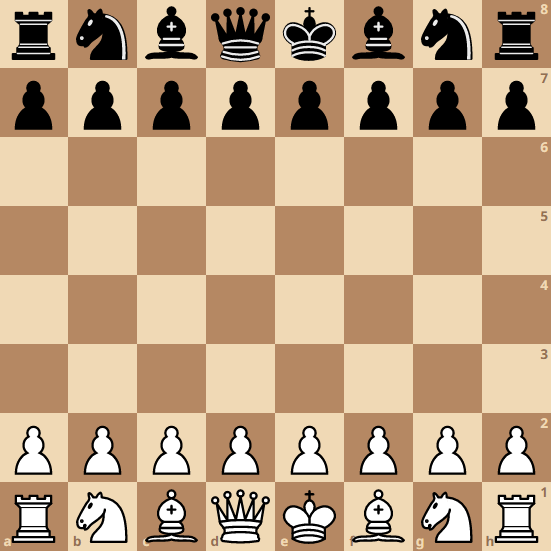
\includegraphics{../Abbildungen/Grundaufstellung.png}
\caption{Grundaufstellung}
\end{figure}

    \hypertarget{bewegungsmuxf6glichkeiten-der-figuren}{%
\subsubsection{Bewegungsmöglichkeiten der
Figuren}\label{bewegungsmuxf6glichkeiten-der-figuren}}

Jede der bereits genannten Figuren hat einen Wert und ein
Bewegungsmuster. Figuren können im Rahmen dieses Bewegungsmuster bewegt
werden, werden aber durch andere Figuren blockiert. Eine Figur kann nur
in Ausnahmefällen übersprungen werden und blockiert grundsätzlich die
Bewegungen aller anderen Figuren. Figuren des Gegners (der anderen
Farbe) können geschlagen werden, indem eine eigene Figur auf dasselbe
Feld gestellt wird. Eine geschlagene Figur wird vom Spielfeld entfernt.
Zwei Figuren derselben Farbe können nicht auf demselben Feld platziert
werden. Diese lauten wie folgt (Jonathan Carlstedt, Die kleine
Schachschule (2015): S.10ff., S.40): 
\begin{itemize}
	\item 
		\textbf{König} (unendlich): Der
		König gehört zu den unbeweglichsten Figuren auf dem Spielfeld. Er kann
		pro Zug nur ein Feld entlang einer Reihe, Linie oder Diagonalen bewegt
		werden. Dadurch besitzt er jedoch die Möglichkeit, in jede Richtung eine
		gegnerische Figur zu schlagen. Als weitere Einschränkung muss beim
		Ziehen mit dem König beachtet werden, dass das angestrebte Feld nicht
		durch eine gegnerische Figur abgedeckt wird. Ein Feld gilt als
		abgedeckt, wenn eine gegnerische Figur es in einem Zug betreten und die
		darauf stehende Figur schlagen kann. Ist dies der Fall, darf der König
		nicht auf dieses Feld gesetzt werden.
		\begin{figure}
			\centering
			\includegraphics{../Abbildungen/König.png} 
			\caption{Bewegungsmuster König}
		\end{figure}
	\item 
		\textbf{Turm} (5): Der Turm
		besitzt die Möglichkeit, in einer Reihe oder Linie beliebig viele Felder
		zu überqueren (maximal bis zum Ende des Spielfeldes).
		
		\begin{figure}
			\centering
			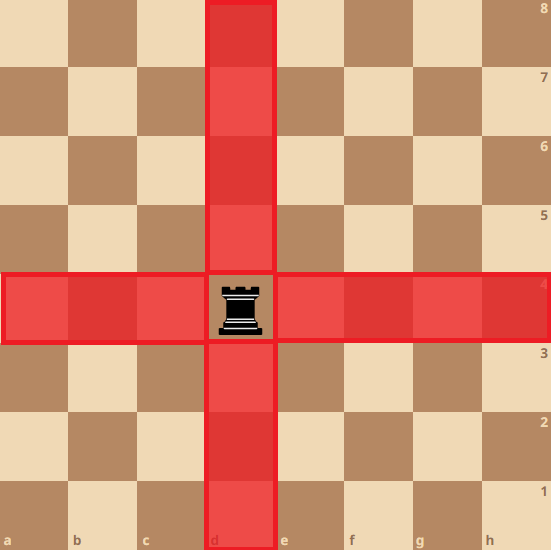
\includegraphics{../Abbildungen/Turm.png} 
			\caption{Bewegungsmuster Turm}
		\end{figure}
	
	\item 
		\textbf{Läufer} (3): Der
		Läufer kann wie ein Turm in geraden Linien bewegt werden. Er
		unterscheidet sich dadurch, dass er nur diagonal bewegt werden kann. Ein
		Läufer auf dem Feld ``a1'' kann folglich nur nach ``b2'' oder entlang
		der Diagonale bewegt werden. 
		
		\begin{figure}
			\centering
			\includegraphics{../Abbildungen/Läufer.png} 
			\caption{Bewegungsmuster Läufer}
		\end{figure}
	
	\item 
		\textbf{Dame} (9): Die Dame zählt zu den beweglichsten Figuren auf dem
		Spielfeld. Sie kombiniert die Bewegungsmuster des Läufers und des Turms.
		Das bedeutet, dass sie horizontal (entlang der Reihen), vertikal
		(entlang der Linien) und diagonal bewegt werden kann.
		
		\begin{figure}
			\centering
			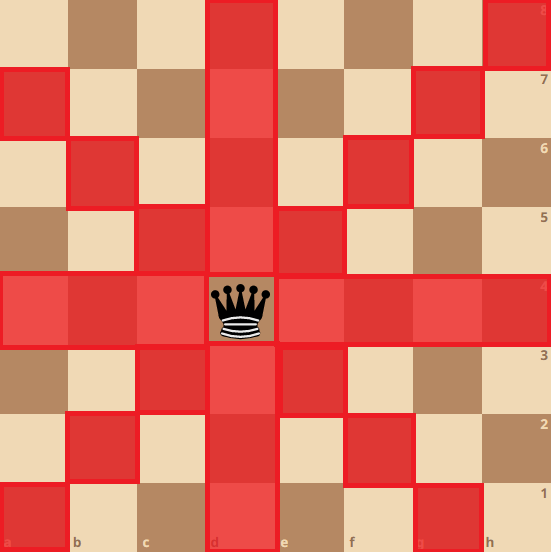
\includegraphics{../Abbildungen/Dame.png} 
			\caption{Bewegungsmuster Dame}
		\end{figure}
	
	\item
		\textbf{Bauer} (1): Der
		Bauer ist die Figur mit der geringsten Beweglichkeit. Dieser kann nur
		entlang der Linie nach vorne bewegt werden. Die erste Bewegung jedes
		Bauern kann ein oder zwei Felder weit sein, folgende Bewegungen sind
		immer genau ein Feld weit. Eine Besonderheit des Bauerns, liegt in der
		Richtung, in die ein Bauer gegnerische Figuren schlagen darf. Dieser
		darf nur diagonal nach vorne schlagen. Weiter wird der Bauer in eine
		beliebige Spielfigur (außer einem Bauern und einem zweiten König)
		gewandelt, sobald er die Grundlinie des Gegners erreicht hat.
		
		\begin{figure}
			\centering
			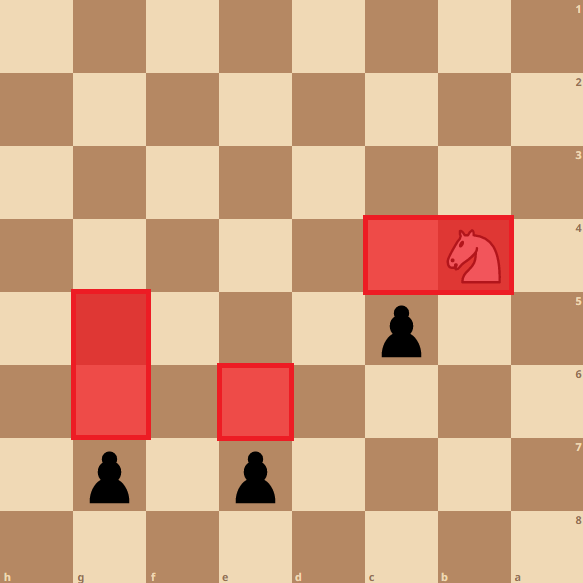
\includegraphics{../Abbildungen/Bauer.png} 
			\caption{Bewegungsmuster Bauer}
		\end{figure}
	
	\item
		\textbf{Springer} (3): Der
		Springer besitzt im Gegensatz zu allen bereits beschriebenen Figuren
		keine lineare Bewegungsrichtung. Er kann um zwei Felder nach vorne und
		ein Feld zur Seite versetzt werden. Dieses Verfahren gilt in jede
		Richtung, sodass der Springer im Optimalfall acht Felder erreichen kann.
		Der Name des Springers kommt dadurch zustande, dass er die einzige Figur
		ist, die andere Figuren überspringen kann. Nur das ``Zielfeld'' kann
		durch eine eigene Figur blockiert werden.
		
		\begin{figure}
			\centering
			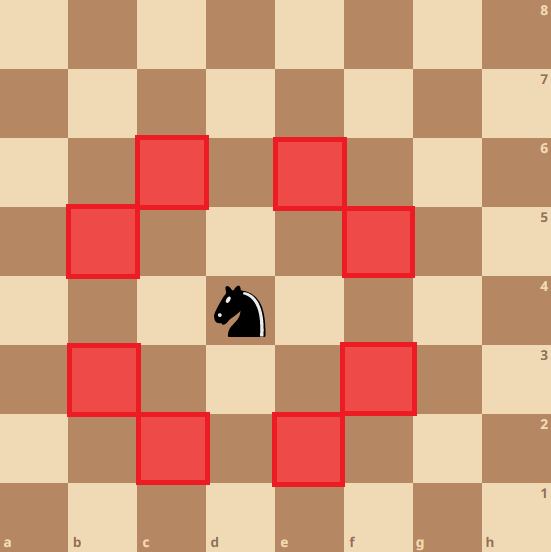
\includegraphics{../Abbildungen/Springer.png} 
			\caption{Bewegungsmuster Soringer}
		\end{figure}
\end{itemize}


    \hypertarget{spielablauf}{%
\subsection{Spielablauf}\label{spielablauf}}

    In einem Spiel ziehen die Spieler immer abwechselnd eine Figur ihrer
Farbe. Den ersten Zug hat dabei immer weiß.

Beide Spieler verfolgen während der ganzen Partie das Ziel, den
gegnerischen Spieler Schach-Matt zu setzen. Ein Spieler ist Schach-Matt,
wenn folgende Bedingungen erfüllt sind: 1. Der König wird durch eine
gegnerische Figur bedroht. 2. Der König kann dieser Bedrohung nicht
ausweichen.

Eine solche Bedrohung liegt vor, wenn der gegnerische Spieler im
nächsten Zug den König schlagen kann. Dies kann auf drei
unterschiedliche Weisen pariert werden: 1. Der König bewegt sich aus dem
``Schach''. 2. Der Spieler schlägt die Schach-gebende Figur. 3. Eine
Figur stellt sich zwischen die Schach-gebende Figur und den König.

Ein anderer Spielausgang neben dem Schach-Matt liegt in dem Patt. Ein
Patt ist dann gegeben, wenn der Spieler, der am Zug ist, keine Figur
mehr ziehen kann und der König des Ziehenden nicht im Schach steht.

    Da diese Studienarbeit nicht vorsieht, das komplette Schachspiel zu
erklären, werden die restlichen Spielregeln nicht näher erläutert. Diese
werden aber in der
\href{https://python-chess.readthedocs.io/en/latest/}{python-chess}
Bibliothek, welche für die Abbildung des Schachspiels im Code verwendet
wird, umgesetzt und berücksichtigt.

    Anhand der Nummerierung der Notebooks können nun die einzelnen Schritte
zur Erstellung und Validierung einer Schach-Endspiel-KI nachvollzogen
werden. Die einzelnen Notebooks begleiten chronologisch die Erstellung,
Validierung und Verwendung einer Endspiel-KI. Die hierfür notwendigen
Notebooks sind:

\begin{enumerate}
\def\labelenumi{\arabic{enumi}.}
\tightlist
\item
  02\_calculation.ipynb
\item
  03\_play\_against\_ai.ipynb
\item
  04\_play\_from\_history.ipynb
\item
  05\_stockfish\_compare.ipynb
\item
  06\_validate\_sequences.ipynb
\end{enumerate}

Im Util-Ordner werden zusätzlich allgemeine Importe und Funktionen
aufgelistet, die für die Ausführung der aufgelisteten Notebooks benötigt
werden.

In der PDF-Version dieser Arbeit ist jedes der aufgelisteten Notebooks
ein Kapitel.

    \hypertarget{berechnung-der-endspieldatenbank}{%
\section{Berechnung der
Endspieldatenbank}\label{berechnung-der-endspieldatenbank}}

Wie in Notebook \texttt{01\_chess\_introduction} bereits erklärt, ist
ein Schachspiel gewonnen, wenn die gegnerische Figur mattgesetzt wurde.

Bei einer geringen Anzahl an Figuren \(P\) im Spielzustand lassen sich
alle möglichen Positionen berechnen. Aus diesen kann eine Strategie
entwickelt werden, den Gegner zu schlagen.

Im weiteren Verlauf werden folgende Definitionen verwendet: 
\begin{itemize}
	\item \(board.pieces\): Liste der Figuren, welche in einem Zustand vorhanden sind. 
	\item \(valid\_boards\): Alle Zustände des Schachspiels, die gegen keine Regeln verstoßen. 
	\item \(won\_boards\): Alle Zustände des Schachspiels, in denen ein Spieler gewonnen hat. 
	\item \(previous\_states(b)\): Alle Zustände, aus denen durch Ausführen eines einzelnen Zuges der Zustand \(b\) erreicht werden kann.
\end{itemize}


Seien alle möglichen (validen) Kombinationen von Positionen der Figuren
\(P\) die Menge \(S\).\\
Für \(S\) gilt:\\
\[
board \in S \implies \forall p \in P : p \in board.pieces \\
\land \\
board \in S \implies board \in valid\_Boards
\]

Aus der Menge \(S\) lassen sich Zustände auswählen, welche \(n\) Züge
vom Sieg entfernt sind. Diese Zustände lassen sich in \(S_n\)
zusammenfassen. Ist das Spiel gewonnen, verbleiben 0 Züge bis zum
Sieg.\\
Für alle diese Zustände, in denen ein Spieler mattgesetzt ist, gilt:\\
\[
board \in S_0 \implies board \in won\_boards \land board \in S
\] Aus dieser Definition können induktiv die verbleibenden \(S_n\)
hergeleitet werden:\\
\[board \in S_{n+1} \iff board \in S \land \exists b \in S_n: board \in previous\_states(b)\]

Für die Berechnungen in diesem Notebook gilt da für den schwarzen
Spieler immer nur der König auf dem Feld steht weiter Folgendes:\\
\(board.turn\): Der Spieler, welcher am Zug ist.

\[
n \equiv 0 \mod 2 \implies \forall b \in S_n : b.turn = schwarz \\
\]
\[
\land 
\]
\[ 
n \equiv 1 \mod 2 \implies \forall b \in S_n : b.turn = weiss \\
\]

Dieses Notebook wird zur Berechnung der \(S_n\) Mengen verwendet. Diese
werden benötigt, um letztendlich ein Schach-Endspiel lösen zu können.

    \hypertarget{ein-hinweis-zu-spiegelungen}{%
\subsection{Ein Hinweis zu
Spiegelungen}\label{ein-hinweis-zu-spiegelungen}}

In diesem Notebook werden Spiegelungen der Situationen verwendet. Die
technische Umsetzung dieser Spiegelungen werden im Verlauf des Dokuments
erklärt, an dieser Stelle soll lediglich eine Einführung in die Theorie
hinter dem Spiegeln von Situationen erklärt werden.

Durch die zuvor erklärten Bewegungsmuster der Figuren sind Schachbretter
in vielen Fällen symmetrisch.

Eine Position mit dem Turm in ``a8'', der Dame in ``g6'' und dem
gegnerischen König in ``h8'' ist genauso verloren wie dieselbe Position
nur mit dem Turm in ``a1'', der Dame in ``g3'' und dem König in ``h1''.
Dies wäre eine Spiegelung entlang der horizontalen zwischen den Zeilen 4
und 5. Weiter sind auch Spiegelungen entlang der vertikalen (Zwischen
Reihe e und f), den Diagonalen und Rotationen (jeweils um 90°, 180° und
270°) möglich.

Durch das simple Spiegeln der Spielsituationen können aus einer validen
Spielsituation bis zu sieben weitere ohne großen Rechenaufwand
erstellen. Aus diesem Grund werden in diesem Dokument bei jeder
Berechnung neuer Situationen diese gespiegelt und die Spiegelungen
ebenfalls überprüft und abgespeichert.

Da Bauern sich nur in eine Richtung bewegen können, werden nur
Spielsituationen gespiegelt, welche keine Bauern enthalten.

    \hypertarget{ein-hinweis-zur-effizienten-ergebnisverwaltung}{%
\subsection{Ein Hinweis zur effizienten
Ergebnisverwaltung}\label{ein-hinweis-zur-effizienten-ergebnisverwaltung}}

Im Verlauf der Berechnung muss mehrfach überprüft werden, ob eine
Situation bereits bekannt und einem \(S_n\) zugeordnet ist. Da der
Abgleich mit einer Liste in Python ineffizient ist, findet dieser
Abgleich mit Mengen statt. Mengen werden in Python als Hash-Tabellen
umgesetzt und haben damit eine Zeitkomplexität bei der Überprüfung, ob
sie ein bestimmtes Element enthalten von \(\mathcal{O}(1)\).
\texttt{board} Objekte der \texttt{chess} Library sind jedoch nicht
``Hashbar''. Im Sinne der in dieser Arbeit getätigten Berechnungen
reichen die Informationen über die Stellung der Figuren und dem Spieler,
welcher am Zug ist, aus. Es wird daher für die Verwendung in Python
Mengen mit einer Tupel-Repräsentation der Situationen wie folgt
gearbeitet: \[
Tupel := <board.turn, board.\_\_str\_\_()>
\] Die Funktion \texttt{board.\_\_str\_\_()} gibt einen String zurück,
welcher ein Schachbrett wie folgt darstellt:

\begin{verbatim}
'r n b q k b n r\np p p p p p p p\n. . . . . . . .\n. . . . . . . . 
\end{verbatim}
\begin{verbatim}
\n. . . . . . . .\n. . . . . . . .\nP P P P P P P P\nR N B Q K B N R'
\end{verbatim}

Die Eigenschaft \texttt{board.turn} ist ein boolscher Wert. Sowohl
Tupel, als auch Strings und boolsche Werte sind in Python ``Hashable'',
weshalb diese Darstellung in Mengen verwendet werden kann.

Um die Effizienz weiter zu steigern, berechnet dieses Notebook nicht
alle Situationen \(S\) und entfernt daraus die Situationen für ein
\(S_n\) wie in der Aufgabenstellung beschrieben. Stattdessen werden alle
bekannten Situationen in \texttt{used\_boards} gespeichert. Dopplungen
werden also nicht vermieden indem Situationen aus einer großen Liste
entfernt werden, sondern eine Liste der entfernten Situationen geführt
und neue Situationen mit dieser abgeglichen.

    \hypertarget{funktionen-zur-bestimmung-aller-guxfcltigen-positionen}{%
\subsection{Funktionen zur Bestimmung aller gültigen
Positionen}\label{funktionen-zur-bestimmung-aller-guxfcltigen-positionen}}

Wie bereits in \texttt{01\_chess\_introduction} beschrieben, besteht ein
Schachbrett aus insgesamt acht Spalten und Zeilen. Die Spalten werden
durch Buchstaben gekennzeichnet, die Zeilen durch Zahlen. Aus der
Kombination einer Spalte (z.B. a) und einer Zahl (z.B. 1) erhält man
eine eindeutige Kennzeichnung für ein Feld (z.B. a1).\\
Die folgende Funktion kombiniert die Buchstaben a bis h mit den Zahlen 1
bis 8 zu Feldnamen und gibt diese zurück.

    \begin{tcolorbox}[breakable, size=fbox, boxrule=1pt, pad at break*=1mm,colback=cellbackground, colframe=cellborder]
\prompt{In}{incolor}{ }{\boxspacing}
\begin{Verbatim}[commandchars=\\\{\}]
\PY{k}{def} \PY{n+nf}{get\PYZus{}all\PYZus{}squares}\PY{p}{(}\PY{p}{)}\PY{p}{:}
    \PY{n}{columns} \PY{o}{=} \PY{p}{\PYZob{}}
        \PY{l+m+mi}{1} \PY{p}{:} \PY{l+s+s1}{\PYZsq{}}\PY{l+s+s1}{a}\PY{l+s+s1}{\PYZsq{}}\PY{p}{,}
        \PY{l+m+mi}{2} \PY{p}{:} \PY{l+s+s1}{\PYZsq{}}\PY{l+s+s1}{b}\PY{l+s+s1}{\PYZsq{}}\PY{p}{,}
        \PY{l+m+mi}{3} \PY{p}{:} \PY{l+s+s1}{\PYZsq{}}\PY{l+s+s1}{c}\PY{l+s+s1}{\PYZsq{}}\PY{p}{,}
        \PY{l+m+mi}{4} \PY{p}{:} \PY{l+s+s1}{\PYZsq{}}\PY{l+s+s1}{d}\PY{l+s+s1}{\PYZsq{}}\PY{p}{,}
        \PY{l+m+mi}{5} \PY{p}{:} \PY{l+s+s1}{\PYZsq{}}\PY{l+s+s1}{e}\PY{l+s+s1}{\PYZsq{}}\PY{p}{,}
        \PY{l+m+mi}{6} \PY{p}{:} \PY{l+s+s1}{\PYZsq{}}\PY{l+s+s1}{f}\PY{l+s+s1}{\PYZsq{}}\PY{p}{,}
        \PY{l+m+mi}{7} \PY{p}{:} \PY{l+s+s1}{\PYZsq{}}\PY{l+s+s1}{g}\PY{l+s+s1}{\PYZsq{}}\PY{p}{,}
        \PY{l+m+mi}{8} \PY{p}{:} \PY{l+s+s1}{\PYZsq{}}\PY{l+s+s1}{h}\PY{l+s+s1}{\PYZsq{}}
    \PY{p}{\PYZcb{}}
    
    \PY{n}{all\PYZus{}squares} \PY{o}{=} \PY{p}{[}\PY{p}{]}
    \PY{k}{for} \PY{n}{row} \PY{o+ow}{in} \PY{n+nb}{range}\PY{p}{(}\PY{l+m+mi}{1}\PY{p}{,}\PY{l+m+mi}{9}\PY{p}{)}\PY{p}{:}
        \PY{k}{for} \PY{n}{col\PYZus{}num} \PY{o+ow}{in} \PY{n+nb}{range}\PY{p}{(}\PY{l+m+mi}{1}\PY{p}{,}\PY{l+m+mi}{9}\PY{p}{)}\PY{p}{:}
            \PY{n}{column} \PY{o}{=} \PY{n}{columns}\PY{p}{[}\PY{n}{col\PYZus{}num}\PY{p}{]}
            \PY{n}{all\PYZus{}squares}\PY{o}{.}\PY{n}{append}\PY{p}{(}\PY{n}{chess}\PY{o}{.}\PY{n}{parse\PYZus{}square}\PY{p}{(}\PY{n}{column} \PY{o}{+} \PY{n+nb}{str}\PY{p}{(}\PY{n}{row}\PY{p}{)}\PY{p}{)}\PY{p}{)}
            
    \PY{k}{return} \PY{n}{all\PYZus{}squares}
\end{Verbatim}
\end{tcolorbox}

    Das Erstellen jeglicher Boards wird mit der Funktion
\texttt{place\_piece\_everywhere\_on\_every\_board} umgesetzt. Diese
erhält folgende Parameter:

\begin{itemize}
\tightlist
\item
  \texttt{piece}: Die zu platzierende Figur als Objekt der
  chess-Library.
\item
  \texttt{list\_of\_boards}: Eine Liste mit Board-Objekten, auf welchen
  die Figur platziert werden soll.
\end{itemize}

Die Funktion betrachtet jede Situation in der \texttt{list\_of\_boards}.
Das übergebene \texttt{piece} wird auf jeden freien Platz dieser
Situation platziert. Jedes Mal, wenn eine Figur platziert wird, wird
eine Kopie des Board-Objektes erstellt, die \texttt{list\_of\_boards}
wird folglich nicht verändert.\\
Wenn der zweite König platziert wird, wird die Situation zusätzlich auf
Validität überprüft. Wenn alle Figuren platziert wurden, werden nur
Boards, in denen Schwarz matt ist, zurückgegeben.

Um die Effizienz der Berechnung zu erhöhen, werden die Schachbretter
gespiegelt. Damit bei folgenden Berechnungen Situationen nicht einmal
durch Spiegelung und einmal durch Bewegung von Figuren erreicht werden,
werden die ungespiegelten Situationen in der Liste \texttt{uniques}
gespeichert.

Die Funktion gibt als Ergebnis eine Liste aller generierten Zustände als
\texttt{result\_list}, die Menge der bereits verwendeten Situationen
\texttt{used\_boards} und alle ungespiegelten Boards (vor Spiegelungen)
\texttt{uniques} zurück.

    \begin{tcolorbox}[breakable, size=fbox, boxrule=1pt, pad at break*=1mm,colback=cellbackground, colframe=cellborder]
\prompt{In}{incolor}{ }{\boxspacing}
\begin{Verbatim}[commandchars=\\\{\}]
\PY{k}{def} \PY{n+nf}{place\PYZus{}figure\PYZus{}everywhere\PYZus{}on\PYZus{}every\PYZus{}board}\PY{p}{(}\PY{n}{piece}\PY{p}{,} \PY{n}{list\PYZus{}of\PYZus{}boards}\PY{p}{,} \PY{n}{piece\PYZus{}count}\PY{p}{,} \PY{n}{user\PYZus{}wants\PYZus{}pawn}\PY{p}{)}\PY{p}{:}
    \PY{n}{result\PYZus{}list} \PY{o}{=} \PY{p}{[}\PY{p}{]}
    \PY{n}{uniques} \PY{o}{=} \PY{p}{[}\PY{p}{]}
    \PY{n}{all\PYZus{}squares} \PY{o}{=} \PY{n}{get\PYZus{}all\PYZus{}squares}\PY{p}{(}\PY{p}{)}
    \PY{n}{used\PYZus{}boards} \PY{o}{=} \PY{n+nb}{set}\PY{p}{(}\PY{p}{)}
    
    \PY{k}{for} \PY{n}{board} \PY{o+ow}{in} \PY{n}{list\PYZus{}of\PYZus{}boards}\PY{p}{:}
        \PY{n}{squares\PYZus{}used} \PY{o}{=} \PY{n+nb}{list}\PY{p}{(}\PY{n}{board}\PY{o}{.}\PY{n}{piece\PYZus{}map}\PY{p}{(}\PY{p}{)}\PY{o}{.}\PY{n}{keys}\PY{p}{(}\PY{p}{)}\PY{p}{)}
        \PY{k}{for} \PY{n}{square} \PY{o+ow}{in} \PY{n}{all\PYZus{}squares}\PY{p}{:}
            \PY{k}{if} \PY{n}{square} \PY{o+ow}{not} \PY{o+ow}{in} \PY{n}{squares\PYZus{}used}\PY{p}{:}
                \PY{n}{tmp\PYZus{}board} \PY{o}{=} \PY{n}{board}\PY{o}{.}\PY{n}{copy}\PY{p}{(}\PY{p}{)}
                \PY{n}{tmp\PYZus{}board}\PY{o}{.}\PY{n}{set\PYZus{}piece\PYZus{}at}\PY{p}{(}\PY{n}{square}\PY{p}{,} \PY{n}{piece}\PY{p}{)}
                
                \PY{k}{if} \PY{n+nb}{len}\PY{p}{(}\PY{n}{squares\PYZus{}used}\PY{p}{)} \PY{o}{\PYZgt{}} \PY{l+m+mi}{1} \PY{o+ow}{and} \PY{o+ow}{not} \PY{n}{tmp\PYZus{}board}\PY{o}{.}\PY{n}{is\PYZus{}valid}\PY{p}{(}\PY{p}{)}\PY{p}{:} 
                    \PY{c+c1}{\PYZsh{} Don\PYZsq{}t process invalid boards further }
                    \PY{c+c1}{\PYZsh{} than the second king}
                    \PY{k}{continue}
                    
                \PY{n}{outcome} \PY{o}{=} \PY{n}{tmp\PYZus{}board}\PY{o}{.}\PY{n}{outcome}\PY{p}{(}\PY{p}{)}
                \PY{k}{if} \PY{n}{outcome} \PY{o+ow}{is} \PY{o+ow}{not} \PY{k+kc}{None}\PY{p}{:}
                    \PY{n}{rep} \PY{o}{=} \PY{p}{(}\PY{n}{tmp\PYZus{}board}\PY{o}{.}\PY{n}{turn}\PY{p}{,} \PY{n}{tmp\PYZus{}board}\PY{o}{.}\PY{n+nf+fm}{\PYZus{}\PYZus{}str\PYZus{}\PYZus{}}\PY{p}{(}\PY{p}{)}\PY{p}{)}
                    \PY{k}{if} \PY{n}{outcome}\PY{o}{.}\PY{n}{winner} \PY{o+ow}{is} \PY{o+ow}{not} \PY{k+kc}{None} \PY{o+ow}{and} \PY{n}{tmp\PYZus{}board}\PY{o}{.}\PY{n}{is\PYZus{}valid}\PY{p}{(}\PY{p}{)} \PY{o+ow}{and} \PY{n}{rep} \PY{o+ow}{not} \PY{o+ow}{in} \PY{n}{used\PYZus{}boards}\PY{p}{:}
                        \PY{n}{uniques}\PY{o}{.}\PY{n}{append}\PY{p}{(}\PY{n}{tmp\PYZus{}board}\PY{p}{)}
                        \PY{n}{result\PYZus{}list}\PY{o}{.}\PY{n}{append}\PY{p}{(}\PY{n}{tmp\PYZus{}board}\PY{p}{)}
                        \PY{n}{used\PYZus{}boards}\PY{o}{.}\PY{n}{add}\PY{p}{(}\PY{p}{(}\PY{n}{tmp\PYZus{}board}\PY{o}{.}\PY{n}{turn}\PY{p}{,}\PY{n}{tmp\PYZus{}board}\PY{o}{.}\PY{n+nf+fm}{\PYZus{}\PYZus{}str\PYZus{}\PYZus{}}\PY{p}{(}\PY{p}{)}\PY{p}{)}\PY{p}{)}
                        \PY{k}{if} \PY{o+ow}{not} \PY{n}{user\PYZus{}wants\PYZus{}pawn}\PY{p}{:}
                            \PY{k}{for} \PY{n}{swt} \PY{o+ow}{in} \PY{n}{Swap\PYZus{}Type}\PY{p}{:}
                                \PY{n}{mir\PYZus{}board} \PY{o}{=} \PY{n}{mirror}\PY{p}{(}\PY{n}{tmp\PYZus{}board}\PY{p}{,} \PY{n}{swt}\PY{p}{)}
                                \PY{k}{if} \PY{p}{(}\PY{n}{mir\PYZus{}board}\PY{o}{.}\PY{n}{turn}\PY{p}{,} \PY{n}{mir\PYZus{}board}\PY{o}{.}\PY{n+nf+fm}{\PYZus{}\PYZus{}str\PYZus{}\PYZus{}}\PY{p}{(}\PY{p}{)}\PY{p}{)} \PY{o+ow}{not} \PY{o+ow}{in} \PY{n}{used\PYZus{}boards}\PY{p}{:}
                                    \PY{n}{result\PYZus{}list}\PY{o}{.}\PY{n}{append}\PY{p}{(}\PY{n}{mir\PYZus{}board}\PY{p}{)}
                                    \PY{n}{used\PYZus{}boards}\PY{o}{.}\PY{n}{add}\PY{p}{(}\PY{p}{(}\PY{n}{mir\PYZus{}board}\PY{o}{.}\PY{n}{turn}\PY{p}{,}\PY{n}{mir\PYZus{}board}\PY{o}{.}\PY{n+nf+fm}{\PYZus{}\PYZus{}str\PYZus{}\PYZus{}}\PY{p}{(}\PY{p}{)}\PY{p}{)}\PY{p}{)}
                        \PY{k}{continue}
                        
                \PY{k}{if} \PY{n+nb}{len}\PY{p}{(}\PY{n}{squares\PYZus{}used}\PY{p}{)} \PY{o}{+} \PY{l+m+mi}{1} \PY{o}{\PYZlt{}} \PY{n}{piece\PYZus{}count}\PY{p}{:} \PY{c+c1}{\PYZsh{}Board is valid, but needs more pieces}
                    \PY{n}{result\PYZus{}list}\PY{o}{.}\PY{n}{append}\PY{p}{(}\PY{n}{tmp\PYZus{}board}\PY{p}{)}
    \PY{k}{return} \PY{n}{result\PYZus{}list}\PY{p}{,} \PY{n}{used\PYZus{}boards}\PY{p}{,} \PY{n}{uniques}
\end{Verbatim}
\end{tcolorbox}

    \hypertarget{die-ursprungsmenge-s_0-erstellen}{%
\subsection{\texorpdfstring{Die Ursprungsmenge \(S_0\)
erstellen}{Die Ursprungsmenge S\_0 erstellen}}\label{die-ursprungsmenge-s_0-erstellen}}

Als Basis der Berechnung dient die Liste \(S_0\). Diese enthält alle
möglichen Konstellationen der Spielfiguren auf dem Spielbrett, in denen
Weiß Schwarz besiegt hat. Hierfür werden die Figuren mit der Funktion
\texttt{place\_figure\_everywhere\_on\_every\_board} auf allen
Positionen platziert.

Die Funktion \texttt{setup\_boards} automatisiert dies und gibt die
Liste \(S_0\), eine Menge der bereits bekannten Situationen
\texttt{used\_boards} und die Menge der ungespiegelten Situationen
\texttt{uniques} zurück.

    \begin{tcolorbox}[breakable, size=fbox, boxrule=1pt, pad at break*=1mm,colback=cellbackground, colframe=cellborder]
\prompt{In}{incolor}{ }{\boxspacing}
\begin{Verbatim}[commandchars=\\\{\}]
\PY{k}{def} \PY{n+nf}{setup\PYZus{}boards}\PY{p}{(}\PY{n}{user\PYZus{}supplied\PYZus{}pieces}\PY{p}{,} \PY{n}{user\PYZus{}wants\PYZus{}pawn}\PY{p}{)}\PY{p}{:}
    \PY{n}{pieces\PYZus{}to\PYZus{}place} \PY{o}{=} \PY{n}{create\PYZus{}piece\PYZus{}list}\PY{p}{(}\PY{n}{user\PYZus{}supplied\PYZus{}pieces}\PY{p}{)}
    
    \PY{n}{empty\PYZus{}board} \PY{o}{=} \PY{n}{chess}\PY{o}{.}\PY{n}{Board}\PY{p}{(}\PY{p}{)}\PY{o}{.}\PY{n}{empty}\PY{p}{(}\PY{p}{)}
    \PY{n}{empty\PYZus{}board}\PY{o}{.}\PY{n}{turn} \PY{o}{=} \PY{n}{chess}\PY{o}{.}\PY{n}{BLACK}
    \PY{n}{s\PYZus{}0} \PY{o}{=} \PY{p}{[}\PY{n}{empty\PYZus{}board}\PY{p}{]}
    
    \PY{n}{piece\PYZus{}count} \PY{o}{=} \PY{n+nb}{len}\PY{p}{(}\PY{n}{pieces\PYZus{}to\PYZus{}place}\PY{p}{)}
    \PY{k}{for} \PY{n}{piece} \PY{o+ow}{in} \PY{n}{pieces\PYZus{}to\PYZus{}place}\PY{p}{:}
        \PY{n}{s\PYZus{}0}\PY{p}{,} \PY{n}{used\PYZus{}boards}\PY{p}{,} \PY{n}{uniques} \PY{o}{=} \PY{n}{place\PYZus{}figure\PYZus{}everywhere\PYZus{}on\PYZus{}every\PYZus{}board}\PY{p}{(}\PY{n}{piece}\PY{p}{,} \PY{n}{s\PYZus{}0}\PY{p}{,} \PY{n}{piece\PYZus{}count}\PY{p}{,} \PY{n}{user\PYZus{}wants\PYZus{}pawn}\PY{p}{)}

    \PY{n+nb}{print}\PY{p}{(}\PY{n+nb}{str}\PY{p}{(}\PY{n+nb}{len}\PY{p}{(}\PY{n}{s\PYZus{}0}\PY{p}{)}\PY{p}{)} \PY{o}{+} \PY{l+s+s2}{\PYZdq{}}\PY{l+s+s2}{ Boards in S\PYZus{}0}\PY{l+s+s2}{\PYZdq{}}\PY{p}{)}
    \PY{k}{return} \PY{n}{s\PYZus{}0}\PY{p}{,} \PY{n}{used\PYZus{}boards}\PY{p}{,} \PY{n}{uniques}
\end{Verbatim}
\end{tcolorbox}

    Bevor die Boards für \(S_0\) erstellt werden können, müssen die vom
Nutzer getätigten Eingaben zu den zu verwendeten Figuren mit den immer
vorhandenen Figuren kombiniert werden. Weiter wird ein eingegebener
Bauer durch eine Königin ersetzt. Ein Endspiel mit zwei Königen und
einem Bauer kann nicht gewonnen werden, weshalb keine Situationen für
\(S_0\) gefunden werden würden. Die Königin wird später im Ablauf wieder
durch einen Bauern ersetzt. Die Theorie hinter diesem Tausch wird zu
einem späterem Zeitpunkt erklärt.

    \begin{tcolorbox}[breakable, size=fbox, boxrule=1pt, pad at break*=1mm,colback=cellbackground, colframe=cellborder]
\prompt{In}{incolor}{ }{\boxspacing}
\begin{Verbatim}[commandchars=\\\{\}]
\PY{c+c1}{\PYZsh{} A queen will automatically be replaced by a pawn}
\PY{k}{def} \PY{n+nf}{create\PYZus{}piece\PYZus{}list}\PY{p}{(}\PY{n}{user\PYZus{}supplied\PYZus{}pieces}\PY{p}{)}\PY{p}{:}
    \PY{k}{if} \PY{n}{chess}\PY{o}{.}\PY{n}{Piece}\PY{o}{.}\PY{n}{from\PYZus{}symbol}\PY{p}{(}\PY{l+s+s2}{\PYZdq{}}\PY{l+s+s2}{P}\PY{l+s+s2}{\PYZdq{}}\PY{p}{)} \PY{o+ow}{in} \PY{n}{user\PYZus{}supplied\PYZus{}pieces}\PY{p}{:}
        \PY{n}{user\PYZus{}supplied\PYZus{}pieces}\PY{o}{.}\PY{n}{remove}\PY{p}{(}\PY{n}{chess}\PY{o}{.}\PY{n}{Piece}\PY{o}{.}\PY{n}{from\PYZus{}symbol}\PY{p}{(}\PY{l+s+s2}{\PYZdq{}}\PY{l+s+s2}{P}\PY{l+s+s2}{\PYZdq{}}\PY{p}{)}\PY{p}{)}
        \PY{n}{user\PYZus{}supplied\PYZus{}pieces}\PY{o}{.}\PY{n}{append}\PY{p}{(}\PY{n}{chess}\PY{o}{.}\PY{n}{Piece}\PY{o}{.}\PY{n}{from\PYZus{}symbol}\PY{p}{(}\PY{l+s+s2}{\PYZdq{}}\PY{l+s+s2}{Q}\PY{l+s+s2}{\PYZdq{}}\PY{p}{)}\PY{p}{)}
        
    \PY{k}{return} \PY{p}{[}\PY{n}{chess}\PY{o}{.}\PY{n}{Piece}\PY{o}{.}\PY{n}{from\PYZus{}symbol}\PY{p}{(}\PY{l+s+s2}{\PYZdq{}}\PY{l+s+s2}{K}\PY{l+s+s2}{\PYZdq{}}\PY{p}{)}\PY{p}{,} \PY{n}{chess}\PY{o}{.}\PY{n}{Piece}\PY{o}{.}\PY{n}{from\PYZus{}symbol}\PY{p}{(}\PY{l+s+s2}{\PYZdq{}}\PY{l+s+s2}{k}\PY{l+s+s2}{\PYZdq{}}\PY{p}{)}\PY{p}{]} \PYZbs{}
           \PY{o}{+} \PY{n}{user\PYZus{}supplied\PYZus{}pieces}
\end{Verbatim}
\end{tcolorbox}

    \hypertarget{ruxfcckwuxe4rts-neue-situationen-bestimmen}{%
\subsection{Rückwärts neue Situationen
bestimmen}\label{ruxfcckwuxe4rts-neue-situationen-bestimmen}}

Der nächste Schritt besteht darin, sämtliche \(S_{n}\) Mengen zu
bestimmen. Hierzu wird eine bereits bestimmte \(S_n\) Menge genommen und
alle Situationen berechnet, die durch Durchführen eines Zugs zu einer
Situation aus \(S_n\) werden.

Besonders muss bei dieser Art der Bestimmung auf die Einordnung der
Situationen, bei welchen Schwarz am Zug ist, geachtet werden. Da beim
späteren Verwenden der KI die Züge des schwarzen Spielers nicht
beeinflusst werden können, muss jeder mögliche Zug einer Situation in
\(S_{n+1}\) mit \(n \% 2 = 0\) zu einer Situation aus \(S_n\) führen.
Diese Überprüfung wird mit der Funktion
\texttt{check\_black\_determinism} durchgeführt. Da die Züge von Weiß
gezielt gewählt werden können, ist diese Überprüfung bei \(n \% 2 = 1\)
nicht nötig.

Außerdem müssen bei der Durchführung des Algorithmus weitere Aspekte
berücksichtigt werden: 
\begin{itemize}
	\item Da Bauern nur in eine Richtung laufen können,
	müssen die rückwärts Schritte eines Bauern manuell durchgeführt werden.
	Bauern werden daher im ersten Schritt ignoriert. 
	\item Bauern, die die oberste Reihe des Spielfeldes erreichen, können zu einer anderen Figur
	eingetauscht werden. Dieser Schritt wird nicht durch die Pseudo-Legal-Moves abgedeckt, daher wird, sollte sich eine Königin in der obersten Reihe befinden, diese manuell durch einen Bauern ersetzt.
\end{itemize}

Die Umsetzung erfolgt durch die Funktion \texttt{previous\_states}. Alle
Funktionsparameter können aus der nachfolgenden Liste entnommen werden:

\begin{itemize}
\tightlist
\item
  \texttt{used\_boards}: Die Menge aller bereits einem \(n\)
  zugeordneten Situationen, welche nicht noch einmal beachtet werden
  sollen.
\item
  \texttt{iteration\_count}: \(n\) des \(S_n\), welches gerade berechnet
  wird.
\item
  \texttt{user\_wants\_pawn}: Ein Flag, welches steuert, ob spezifische
  Bewegungen des Bauern berechnet werden sollen.
\item
  \texttt{uniques}: Die Situationen, welche als Ursprung der Spiegelung
  verwendet werden.
\end{itemize}

Der Algorithmus zur Bestimmung der Menge \(S_{n+1}\) wird im folgenden
Abschnitt beschrieben. Um die Funktion übersichtlicher zu halten, wurden
teile des Algorithmus in die Funktion \texttt{moves} übertragen.

\begin{itemize}
\tightlist
\item
  Über die Uniques (ungespiegelte Situationen) iterieren.

  \begin{itemize}
  \tightlist
  \item
    Den Spieler, welcher am Zug ist, wechseln (Da, um im aktuellen
    Zustand anzukommen, der andere Spieler einen Zug gemacht hat)
  \item
    Alle Positionen mit Bauern berechnen
  \item
    Alle pseudo-legalen Bewegungen mittels der Funktion
    \texttt{regular\_moves} durchführen. Hierbei werden keine Züge der
    Bauern beachtet. Die technische Umsetzung wird in der Dokumentation
    der Funktion erklärt.
  \item
    Wenn die Bewegungen von Bauern abgebildet werden müssen:

    \begin{itemize}
    \tightlist
    \item
      Bauern manuell einen Schritt ``nach hinten'' setzen.
    \item
      Überprüfen, ob eine Dame in der obersten Reihe durch einen Bauern
      in der vorletzten ersetzt werden muss.
    \item
      Die technische Umsetzung dieser Aktionen wird in der Dokumentation
      der Funktionen \texttt{pawn\_moves} und
      \texttt{replace\_queen\_with\_pawn} erklärt.
    \end{itemize}
  \item
    Den Spieler, welcher ursprünglich am Zug war, wiederherstellen.
  \item
    Wenn \((n+1) \% 2 = 0\) überprüfen, ob alle zuvor berechneten Boards
    mit allen Moves in \(S_n\) enden.
  \end{itemize}
\end{itemize}

Außerdem müssen bei der Durchführung des Algorithmus weitere Aspekte
berücksichtigt werden:

\begin{itemize}
\tightlist
\item
  Da Bauern nur in eine Richtung laufen können, müssen die rückwärts
  Schritte eines Bauern manuell durchgeführt werden. Bauern werden daher
  im ersten Schritt ignoriert.
\item
  Bauern, die die oberste Reihe des Spielfeldes erreichen, können zu
  einer anderen Figur eingetauscht werden. Dieser Schritt wird nicht
  durch die Pseudo-Legal-Moves abgedeckt, daher wird, sollte sich eine
  Königin in der obersten Reihe befinden, diese manuell durch einen
  Bauern ersetzt.
\end{itemize}

Die Funktion bestimmt die Menge \(S_{n+1}\), die Menge der bekannten
Boards als Tupel \texttt{used\_boards} und die ungespiegelten Origniale
aus \(n+1\) \texttt{s\_n1\_uniques}

    \begin{tcolorbox}[breakable, size=fbox, boxrule=1pt, pad at break*=1mm,colback=cellbackground, colframe=cellborder]
\prompt{In}{incolor}{ }{\boxspacing}
\begin{Verbatim}[commandchars=\\\{\}]
\PY{k}{def} \PY{n+nf}{previous\PYZus{}states}\PY{p}{(}\PY{n}{used\PYZus{}boards}\PY{p}{,} \PY{n}{iteration\PYZus{}count}\PY{p}{,} \PY{n}{user\PYZus{}wants\PYZus{}pawn}\PY{p}{,} \PY{n}{uniques}\PY{p}{)}\PY{p}{:}
    \PY{c+c1}{\PYZsh{}variables}
    \PY{n}{s\PYZus{}n1} \PY{o}{=} \PY{p}{[}\PY{p}{]}
    \PY{n}{s\PYZus{}n1\PYZus{}tuples} \PY{o}{=} \PY{n+nb}{set}\PY{p}{(}\PY{p}{)}
    \PY{n}{s\PYZus{}n1\PYZus{}uniques} \PY{o}{=} \PY{p}{[}\PY{p}{]}
    \PY{n}{s\PYZus{}n1\PYZus{}uniques\PYZus{}tuples} \PY{o}{=} \PY{n+nb}{set}\PY{p}{(}\PY{p}{)}

    \PY{k}{for} \PY{n}{i} \PY{o+ow}{in} \PY{n+nb}{range}\PY{p}{(}\PY{n+nb}{len}\PY{p}{(}\PY{n}{uniques}\PY{p}{)}\PY{p}{)}\PY{p}{:}
        \PY{n}{status} \PY{o}{=} \PY{l+s+s2}{\PYZdq{}}\PY{l+s+s2}{Calculating S}\PY{l+s+s2}{\PYZdq{}} \PY{o}{+} \PY{n+nb}{str}\PY{p}{(}\PY{n}{iteration\PYZus{}count}\PY{p}{)} \PY{o}{+} \PY{l+s+s2}{\PYZdq{}}\PY{l+s+s2}{ \PYZhy{} Board }\PY{l+s+s2}{\PYZdq{}} \PY{o}{+} \PY{n+nb}{str}\PY{p}{(}\PY{n}{i}\PY{o}{+}\PY{l+m+mi}{1}\PY{p}{)} \PY{o}{+} \PY{l+s+s2}{\PYZdq{}}\PY{l+s+s2}{ of }\PY{l+s+s2}{\PYZdq{}} \PY{o}{+} \PY{n+nb}{str}\PY{p}{(}\PY{n+nb}{len}\PY{p}{(}\PY{n}{uniques}\PY{p}{)}\PY{p}{)} \PY{o}{+} \PY{l+s+s2}{\PYZdq{}}\PY{l+s+s2}{ from S}\PY{l+s+s2}{\PYZdq{}} \PY{o}{+} \PY{n+nb}{str}\PY{p}{(}\PY{n}{iteration\PYZus{}count}\PY{o}{\PYZhy{}}\PY{l+m+mi}{1}\PY{p}{)}
        \PY{n}{clear\PYZus{}output}\PY{p}{(}\PY{n}{wait}\PY{o}{=}\PY{k+kc}{True}\PY{p}{)}
        \PY{n+nb}{print}\PY{p}{(}\PY{n}{status}\PY{p}{)}

        \PY{c+c1}{\PYZsh{} Copy current board and invert the player}
        \PY{n}{chess\PYZus{}board} \PY{o}{=} \PY{n}{uniques}\PY{p}{[}\PY{n}{i}\PY{p}{]}\PY{o}{.}\PY{n}{copy}\PY{p}{(}\PY{p}{)}
        \PY{n}{chess\PYZus{}board}\PY{o}{.}\PY{n}{turn} \PY{o}{=} \PY{n}{chess\PYZus{}board}\PY{o}{.}\PY{n}{turn} \PY{o}{\PYZca{}} \PY{k+kc}{True}

        \PY{c+c1}{\PYZsh{} Find all Pawns}
        \PY{n}{pawn\PYZus{}positions} \PY{o}{=} \PY{n}{find\PYZus{}pawns}\PY{p}{(}\PY{n}{chess\PYZus{}board}\PY{p}{)}
        
        \PY{c+c1}{\PYZsh{} try moves and check if they lead to new boards}
        \PY{n}{s\PYZus{}n1}\PY{p}{,} \PY{n}{s\PYZus{}n1\PYZus{}tuples}\PY{p}{,} \PY{n}{s\PYZus{}n1\PYZus{}uniques}\PY{p}{,} \PY{n}{s\PYZus{}n1\PYZus{}uniques\PYZus{}tuples} \PY{o}{=} \PY{n}{moves}\PY{p}{(}\PY{n}{chess\PYZus{}board}\PY{p}{,} \PY{n}{used\PYZus{}boards}\PY{p}{,} \PY{n}{s\PYZus{}n1\PYZus{}tuples}\PY{p}{,} \PY{n}{pawn\PYZus{}positions}\PY{p}{,} \PY{n}{user\PYZus{}wants\PYZus{}pawn}\PY{p}{,} \PY{n}{s\PYZus{}n1}\PY{p}{,} \PY{n}{s\PYZus{}n1\PYZus{}uniques}\PY{p}{,} \PY{n}{s\PYZus{}n1\PYZus{}uniques\PYZus{}tuples}\PY{p}{)}
            

        \PY{c+c1}{\PYZsh{} Restore the original state of the board}
        \PY{n}{chess\PYZus{}board}\PY{o}{.}\PY{n}{turn} \PY{o}{=} \PY{n}{chess\PYZus{}board}\PY{o}{.}\PY{n}{turn} \PY{o}{\PYZca{}} \PY{k+kc}{True}
        
    \PY{c+c1}{\PYZsh{} Only needed for Black\PYZhy{}Moves}
    \PY{k}{if} \PY{n}{iteration\PYZus{}count} \PY{o}{\PYZpc{}} \PY{l+m+mi}{2} \PY{o}{==} \PY{l+m+mi}{0}\PY{p}{:}
        \PY{n}{clear\PYZus{}output}\PY{p}{(}\PY{n}{wait}\PY{o}{=}\PY{k+kc}{True}\PY{p}{)}
        \PY{n+nb}{print}\PY{p}{(}\PY{l+s+s2}{\PYZdq{}}\PY{l+s+s2}{Calculating S}\PY{l+s+s2}{\PYZdq{}} \PY{o}{+} \PY{n+nb}{str}\PY{p}{(}\PY{n}{iteration\PYZus{}count}\PY{p}{)} \PY{o}{+} \PY{l+s+s2}{\PYZdq{}}\PY{l+s+s2}{ \PYZhy{} Checking Black Moves for determinism}\PY{l+s+s2}{\PYZdq{}}\PY{p}{)}
        
        \PY{n}{s\PYZus{}n1}\PY{p}{,} \PY{n}{s\PYZus{}n1\PYZus{}tuples}\PY{p}{,} \PY{n}{s\PYZus{}n1\PYZus{}uniques} \PY{o}{=} \PY{n}{check\PYZus{}black\PYZus{}determinism}\PY{p}{(}\PY{n}{s\PYZus{}n1}\PY{p}{,} \PY{n}{used\PYZus{}boards}\PY{p}{,} \PY{n}{s\PYZus{}n1\PYZus{}uniques\PYZus{}tuples}\PY{p}{)}

    \PY{n}{clear\PYZus{}output}\PY{p}{(}\PY{n}{wait}\PY{o}{=}\PY{k+kc}{True}\PY{p}{)}
    \PY{n+nb}{print}\PY{p}{(}\PY{l+s+s2}{\PYZdq{}}\PY{l+s+s2}{Done with S}\PY{l+s+s2}{\PYZdq{}} \PY{o}{+} \PY{n+nb}{str}\PY{p}{(}\PY{n}{iteration\PYZus{}count}\PY{p}{)}\PY{p}{)}
    \PY{k}{return} \PY{n}{s\PYZus{}n1}\PY{p}{,} \PY{n}{used\PYZus{}boards} \PY{o}{|} \PY{n}{s\PYZus{}n1\PYZus{}tuples}\PY{p}{,} \PY{n}{s\PYZus{}n1\PYZus{}uniques}
\end{Verbatim}
\end{tcolorbox}

    \hypertarget{hilfsfunktionen-fuxfcr-die-berechnung}{%
\subsection{Hilfsfunktionen für die
Berechnung}\label{hilfsfunktionen-fuxfcr-die-berechnung}}

Die folgenden Funktionen werden zur Berechnung der previous\_states
verwendet. Sie übernehmen dabei diverse Aufgaben wie das Durchführen von
regulären Moves oder das ``manuelle'' Versetzen von Figuren, um eine
andere Situation zu generieren.

    Die Funktion \texttt{moves} führt für eine Situation
\texttt{chess\_board} zunächst Züge mit allen Figuren außer dem Bauern
durch. Wenn der Nutzer einen Bauern in seiner Konfiguration angegeben
hat, werden auch Bauernzüge sowie der Tausch Dame zu Bauer durchgeführt.

    \begin{tcolorbox}[breakable, size=fbox, boxrule=1pt, pad at break*=1mm,colback=cellbackground, colframe=cellborder]
\prompt{In}{incolor}{ }{\boxspacing}
\begin{Verbatim}[commandchars=\\\{\}]
\PY{k}{def} \PY{n+nf}{moves}\PY{p}{(}\PY{n}{chess\PYZus{}board}\PY{p}{,} \PY{n}{used\PYZus{}boards}\PY{p}{,} \PY{n}{s\PYZus{}n1\PYZus{}tuples}\PY{p}{,} \PY{n}{pawn\PYZus{}positions}\PY{p}{,} \PY{n}{user\PYZus{}wants\PYZus{}pawn}\PY{p}{,} \PY{n}{s\PYZus{}n1}\PY{p}{,} \PY{n}{s\PYZus{}n1\PYZus{}uniques}\PY{p}{,} \PY{n}{s\PYZus{}n1\PYZus{}uniques\PYZus{}tuples}\PY{p}{)}\PY{p}{:}
    \PY{n}{tmp\PYZus{}n1}\PY{p}{,} \PY{n}{tmp\PYZus{}n1\PYZus{}tuples}\PY{p}{,} \PY{n}{tmp\PYZus{}uniques}\PY{p}{,} \PY{n}{tmp\PYZus{}uniques\PYZus{}tuples} \PY{o}{=} \PY{n}{regular\PYZus{}moves}\PY{p}{(}\PY{n}{chess\PYZus{}board}\PY{p}{,} \PY{n}{used\PYZus{}boards}\PY{p}{,} \PY{n}{s\PYZus{}n1\PYZus{}tuples}\PY{p}{,} \PY{n}{pawn\PYZus{}positions}\PY{p}{,} \PY{n}{user\PYZus{}wants\PYZus{}pawn}\PY{p}{)}
    \PY{n}{s\PYZus{}n1} \PY{o}{+}\PY{o}{=} \PY{n}{tmp\PYZus{}n1}
    \PY{n}{s\PYZus{}n1\PYZus{}tuples} \PY{o}{|}\PY{o}{=} \PY{n}{tmp\PYZus{}n1\PYZus{}tuples}
    \PY{n}{s\PYZus{}n1\PYZus{}uniques} \PY{o}{+}\PY{o}{=} \PY{n}{tmp\PYZus{}uniques}
    \PY{n}{s\PYZus{}n1\PYZus{}uniques\PYZus{}tuples} \PY{o}{|}\PY{o}{=} \PY{n}{tmp\PYZus{}uniques\PYZus{}tuples}

    \PY{k}{if} \PY{n}{user\PYZus{}wants\PYZus{}pawn} \PY{o+ow}{and} \PY{n}{chess\PYZus{}board}\PY{o}{.}\PY{n}{turn}\PY{p}{:}
        \PY{c+c1}{\PYZsh{} Push all pawns one row back and check if this leads to new boards}
        \PY{k}{if} \PY{n+nb}{len}\PY{p}{(}\PY{n}{pawn\PYZus{}positions}\PY{p}{)} \PY{o}{\PYZgt{}} \PY{l+m+mi}{0}\PY{p}{:}
            \PY{n}{tmp\PYZus{}list}\PY{p}{,} \PY{n}{tmp\PYZus{}set} \PY{o}{=} \PY{n}{pawn\PYZus{}moves}\PY{p}{(}\PY{n}{chess\PYZus{}board}\PY{p}{,} \PY{n}{used\PYZus{}boards}\PY{p}{,} \PY{n}{s\PYZus{}n1\PYZus{}tuples}\PY{p}{)}
            \PY{n}{s\PYZus{}n1} \PY{o}{+}\PY{o}{=} \PY{n}{tmp\PYZus{}list}
            \PY{n}{s\PYZus{}n1\PYZus{}tuples} \PY{o}{|}\PY{o}{=} \PY{n}{tmp\PYZus{}set}
            \PY{n}{s\PYZus{}n1\PYZus{}uniques} \PY{o}{+}\PY{o}{=} \PY{n}{tmp\PYZus{}list}
            \PY{n}{s\PYZus{}n1\PYZus{}uniques\PYZus{}tuples} \PY{o}{|}\PY{o}{=} \PY{n}{tmp\PYZus{}set}
        
        \PY{c+c1}{\PYZsh{} Exchange Queens with Pawns}
        \PY{n}{queen\PYZus{}positions} \PY{o}{=} \PY{n}{check\PYZus{}top\PYZus{}row\PYZus{}for\PYZus{}queen}\PY{p}{(}\PY{n}{chess\PYZus{}board}\PY{p}{)}
        \PY{k}{if} \PY{n}{queen\PYZus{}positions}\PY{p}{:}
            \PY{n}{tmp\PYZus{}list}\PY{p}{,} \PY{n}{tmp\PYZus{}set} \PY{o}{=} \PY{n}{replace\PYZus{}queen\PYZus{}with\PYZus{}pawn}\PY{p}{(}\PY{n}{chess\PYZus{}board}\PY{p}{,} \PY{n}{used\PYZus{}boards}\PY{p}{,} \PY{n}{s\PYZus{}n1\PYZus{}tuples}\PY{p}{,} \PY{n}{queen\PYZus{}positions}\PY{p}{)}
            \PY{n}{s\PYZus{}n1} \PY{o}{+}\PY{o}{=} \PY{n}{tmp\PYZus{}list}
            \PY{n}{s\PYZus{}n1\PYZus{}tuples} \PY{o}{|}\PY{o}{=} \PY{n}{tmp\PYZus{}set}
            \PY{n}{s\PYZus{}n1\PYZus{}uniques} \PY{o}{+}\PY{o}{=} \PY{n}{tmp\PYZus{}list}
            \PY{n}{s\PYZus{}n1\PYZus{}uniques\PYZus{}tuples} \PY{o}{|}\PY{o}{=} \PY{n}{tmp\PYZus{}set}
            
    \PY{k}{return} \PY{n}{s\PYZus{}n1}\PY{p}{,} \PY{n}{s\PYZus{}n1\PYZus{}tuples}\PY{p}{,} \PY{n}{s\PYZus{}n1\PYZus{}uniques}\PY{p}{,} \PY{n}{s\PYZus{}n1\PYZus{}uniques\PYZus{}tuples}
\end{Verbatim}
\end{tcolorbox}

    Die Funktion \texttt{regular\_moves} führt für eine übergebene Situation
\texttt{chess\_board} alle \texttt{pseudo\_legal\_moves} durch, um
mögliche vorhergehende Situationen zu berechnen.\\
Pseudo-Legale-Züge sind Züge, welche die Figuren auf eine Art bewegen,
die der Figur gestattet ist, aber unter Umständen in eine nicht legale
Spielsituation führt. Diese werden verwendet, da nur weil der Move von
\(S_{n+1}\) zu \(S_n\) legal ist, der Zug umgekehrt dies nicht sein
muss.

Ein simples Beispiel: Situation \(S_n\): Ein König befindet sich ein
Feld von einem Schach entfernt.\\
Diese Position kann erreicht worden sein, da der König von einer
Position in \(S_{n+1}\) sich aus diesem Schach herausbewegt hat. Der Zug
``in das Schach'', wäre jedoch nicht legal, weshalb ein Move aus der
Liste der \texttt{pseudo\_legal\_moves} zur Berechnung genommen werden
muss. Dies funktioniert nicht für Bauern, da ein Schritt nach ``hinten''
keine Bewegung ist, welche der Figur zusteht.

Die Funktion überprüft jeden Zug, welcher in der Situation möglich ist.
Wenn die errechnete Situation valide und noch nicht verwendet (überprüft
durch Einträge in \texttt{used\_boards} und \texttt{s\_n1\_tuples}) ist,
wird sie den Rückgabe-Variablen angefügt. Wenn sich keine Bauern auf dem
Spielfeld befinden (\texttt{user\_wants\_pawn}), dann können die
Situationen gespiegelt werden, um weiteren Rechenaufwand zu reduzieren.
Diese Spiegelung findet durch eine Iteration über die später definierten
Swap\_Types statt. Anschließend wird mit der Funktion \texttt{mirror}
die Spiegelung bestimmt, die Validität der Situation überprüft und
ebenfalls an das Ergebnis angefügt.

Nach Abschluss der Berechnungen gibt die Funktion die Liste alle neuen
Situationen (ungespiegelt \texttt{uniques} und gespiegelt
\texttt{new\_boards}) sowie deren Tupel-Repräsentation wieder.

    \begin{tcolorbox}[breakable, size=fbox, boxrule=1pt, pad at break*=1mm,colback=cellbackground, colframe=cellborder]
\prompt{In}{incolor}{ }{\boxspacing}
\begin{Verbatim}[commandchars=\\\{\}]
\PY{k}{def} \PY{n+nf}{regular\PYZus{}moves}\PY{p}{(}\PY{n}{chess\PYZus{}board}\PY{p}{,} \PY{n}{used\PYZus{}boards}\PY{p}{,} \PY{n}{s\PYZus{}n1\PYZus{}tuples}\PY{p}{,} \PY{n}{pawn\PYZus{}positions}\PY{p}{,} \PY{n}{user\PYZus{}wants\PYZus{}pawn}\PY{p}{)}\PY{p}{:}
    \PY{n}{new\PYZus{}boards} \PY{o}{=} \PY{p}{[}\PY{p}{]}
    \PY{n}{new\PYZus{}tuples} \PY{o}{=} \PY{n+nb}{set}\PY{p}{(}\PY{p}{)}
    \PY{n}{new\PYZus{}uniques} \PY{o}{=} \PY{p}{[}\PY{p}{]}
    \PY{n}{new\PYZus{}uniques\PYZus{}tuples} \PY{o}{=} \PY{n+nb}{set}\PY{p}{(}\PY{p}{)}
    \PY{k}{for} \PY{n}{pLMove} \PY{o+ow}{in} \PY{n}{chess\PYZus{}board}\PY{o}{.}\PY{n}{pseudo\PYZus{}legal\PYZus{}moves}\PY{p}{:}
        \PY{k}{if} \PY{n}{chess}\PY{o}{.}\PY{n}{square\PYZus{}name}\PY{p}{(}\PY{n}{pLMove}\PY{o}{.}\PY{n}{from\PYZus{}square}\PY{p}{)} \PY{o+ow}{not} \PY{o+ow}{in} \PY{n}{pawn\PYZus{}positions}\PY{p}{:}
            
            \PY{n}{chess\PYZus{}board}\PY{o}{.}\PY{n}{push}\PY{p}{(}\PY{n}{pLMove}\PY{p}{)}
            
            \PY{n}{chess\PYZus{}board}\PY{o}{.}\PY{n}{turn} \PY{o}{=} \PY{n}{chess\PYZus{}board}\PY{o}{.}\PY{n}{turn} \PY{o}{\PYZca{}} \PY{k+kc}{True}
            \PY{k}{if} \PY{o+ow}{not} \PY{n}{chess\PYZus{}board}\PY{o}{.}\PY{n}{is\PYZus{}valid}\PY{p}{(}\PY{p}{)} \PY{o+ow}{or} \PY{n}{chess\PYZus{}board}\PY{o}{.}\PY{n}{outcome}\PY{p}{(}\PY{p}{)} \PY{o+ow}{is} \PY{o+ow}{not} \PY{k+kc}{None}\PY{p}{:}
                \PY{n}{chess\PYZus{}board}\PY{o}{.}\PY{n}{turn} \PY{o}{=} \PY{n}{chess\PYZus{}board}\PY{o}{.}\PY{n}{turn} \PY{o}{\PYZca{}} \PY{k+kc}{True}
                \PY{n}{chess\PYZus{}board}\PY{o}{.}\PY{n}{pop}\PY{p}{(}\PY{p}{)}
                \PY{k}{continue}
                
            \PY{c+c1}{\PYZsh{} If the new board is found in S, it can be reached in one step}
            \PY{n}{tuple\PYZus{}rep} \PY{o}{=} \PY{p}{(}\PY{n}{chess\PYZus{}board}\PY{o}{.}\PY{n}{turn}\PY{p}{,}\PY{n}{chess\PYZus{}board}\PY{o}{.}\PY{n+nf+fm}{\PYZus{}\PYZus{}str\PYZus{}\PYZus{}}\PY{p}{(}\PY{p}{)}\PY{p}{)}
            \PY{k}{if} \PY{n}{tuple\PYZus{}rep} \PY{o+ow}{not} \PY{o+ow}{in} \PY{n}{used\PYZus{}boards} \PY{o+ow}{and} \PY{n}{tuple\PYZus{}rep} \PY{o+ow}{not} \PY{o+ow}{in} \PY{n}{s\PYZus{}n1\PYZus{}tuples} \PY{o+ow}{and} \PY{n}{tuple\PYZus{}rep} \PY{o+ow}{not} \PY{o+ow}{in} \PY{n}{new\PYZus{}tuples}\PY{p}{:}               
                \PY{n}{new\PYZus{}uniques}\PY{o}{.}\PY{n}{append}\PY{p}{(}\PY{n}{chess\PYZus{}board}\PY{o}{.}\PY{n}{copy}\PY{p}{(}\PY{p}{)}\PY{p}{)}
                \PY{n}{new\PYZus{}uniques\PYZus{}tuples}\PY{o}{.}\PY{n}{add}\PY{p}{(}\PY{n}{tuple\PYZus{}rep}\PY{p}{)}
                
                \PY{n}{new\PYZus{}boards}\PY{o}{.}\PY{n}{append}\PY{p}{(}\PY{n}{chess\PYZus{}board}\PY{o}{.}\PY{n}{copy}\PY{p}{(}\PY{p}{)}\PY{p}{)}
                \PY{n}{new\PYZus{}tuples}\PY{o}{.}\PY{n}{add}\PY{p}{(}\PY{n}{tuple\PYZus{}rep}\PY{p}{)}
                
                \PY{k}{if} \PY{o+ow}{not} \PY{n}{user\PYZus{}wants\PYZus{}pawn}\PY{p}{:}
                    \PY{k}{for} \PY{n}{swtype} \PY{o+ow}{in} \PY{n}{Swap\PYZus{}Type}\PY{p}{:}
                        \PY{n}{mirrored\PYZus{}board} \PY{o}{=} \PY{n}{mirror}\PY{p}{(}\PY{n}{chess\PYZus{}board}\PY{p}{,} \PY{n}{swtype}\PY{p}{)}
                        \PY{n}{tuple\PYZus{}rep\PYZus{}mir} \PY{o}{=} \PY{p}{(}\PY{n}{mirrored\PYZus{}board}\PY{o}{.}\PY{n}{turn}\PY{p}{,}\PY{n}{mirrored\PYZus{}board}\PY{o}{.}\PY{n+nf+fm}{\PYZus{}\PYZus{}str\PYZus{}\PYZus{}}\PY{p}{(}\PY{p}{)}\PY{p}{)}
                        \PY{k}{if} \PY{n}{tuple\PYZus{}rep\PYZus{}mir} \PY{o+ow}{not} \PY{o+ow}{in} \PY{n}{used\PYZus{}boards} \PY{o+ow}{and} \PY{n}{tuple\PYZus{}rep\PYZus{}mir} \PY{o+ow}{not} \PY{o+ow}{in} \PY{n}{s\PYZus{}n1\PYZus{}tuples} \PY{o+ow}{and} \PY{n}{tuple\PYZus{}rep\PYZus{}mir} \PY{o+ow}{not} \PY{o+ow}{in} \PY{n}{new\PYZus{}tuples}\PY{p}{:}
                            \PY{n}{new\PYZus{}boards}\PY{o}{.}\PY{n}{append}\PY{p}{(}\PY{n}{mirrored\PYZus{}board}\PY{o}{.}\PY{n}{copy}\PY{p}{(}\PY{p}{)}\PY{p}{)}
                            \PY{n}{new\PYZus{}tuples}\PY{o}{.}\PY{n}{add}\PY{p}{(}\PY{n}{tuple\PYZus{}rep\PYZus{}mir}\PY{p}{)}
            \PY{n}{chess\PYZus{}board}\PY{o}{.}\PY{n}{turn} \PY{o}{=} \PY{n}{chess\PYZus{}board}\PY{o}{.}\PY{n}{turn} \PY{o}{\PYZca{}} \PY{k+kc}{True}
            \PY{n}{chess\PYZus{}board}\PY{o}{.}\PY{n}{pop}\PY{p}{(}\PY{p}{)}
    
    \PY{k}{return} \PY{n}{new\PYZus{}boards}\PY{p}{,} \PY{n}{new\PYZus{}tuples}\PY{p}{,} \PY{n}{new\PYZus{}uniques}\PY{p}{,} \PY{n}{new\PYZus{}uniques\PYZus{}tuples}
\end{Verbatim}
\end{tcolorbox}

    Wie zuvor bereits erwähnt, ermöglicht die quadratische Natur des
Schachbrettes es das Spielbrett zu spiegeln / rotieren und weitere
Situationen zu erhalten.

Zunächst wird ein Enum erstellt, welches es ermöglicht über die Arten
der Figurenvertauschungen zu iterieren. \texttt{Swap\_Type} übersetzt zu
einem String, welcher im nächsten Schritt als Key für ein Dictionary
verwendet wird.

    \begin{tcolorbox}[breakable, size=fbox, boxrule=1pt, pad at break*=1mm,colback=cellbackground, colframe=cellborder]
\prompt{In}{incolor}{ }{\boxspacing}
\begin{Verbatim}[commandchars=\\\{\}]
\PY{k}{class} \PY{n+nc}{Swap\PYZus{}Type}\PY{p}{(}\PY{n}{Enum}\PY{p}{)}\PY{p}{:}
    \PY{n}{VERTICAL} \PY{o}{=} \PY{l+s+s2}{\PYZdq{}}\PY{l+s+s2}{vertical}\PY{l+s+s2}{\PYZdq{}}
    \PY{n}{HORIZONTAL} \PY{o}{=} \PY{l+s+s2}{\PYZdq{}}\PY{l+s+s2}{horizontal}\PY{l+s+s2}{\PYZdq{}}
    \PY{n}{ROTATE\PYZus{}RIGHT} \PY{o}{=} \PY{l+s+s2}{\PYZdq{}}\PY{l+s+s2}{rotate\PYZus{}right}\PY{l+s+s2}{\PYZdq{}}
    \PY{n}{ROTATE\PYZus{}180} \PY{o}{=} \PY{l+s+s2}{\PYZdq{}}\PY{l+s+s2}{rotate\PYZus{}180}\PY{l+s+s2}{\PYZdq{}}
    \PY{n}{ROTATE\PYZus{}LEFT} \PY{o}{=} \PY{l+s+s2}{\PYZdq{}}\PY{l+s+s2}{rotate\PYZus{}left}\PY{l+s+s2}{\PYZdq{}}
\end{Verbatim}
\end{tcolorbox}

    Für den Tausch wird über jede Figur iteriert und diese an die
entsprechende Position gesetzt. Das Ergebnis wird als
\texttt{Board-Objekt} zurückgegeben.

Die Formeln zum Spiegeln und Rotieren der Spielsituationen wurden
\href{https://www.chessprogramming.org/Flipping_Mirroring_and_Rotating}{dieser
Quelle} entnommen.

    \begin{tcolorbox}[breakable, size=fbox, boxrule=1pt, pad at break*=1mm,colback=cellbackground, colframe=cellborder]
\prompt{In}{incolor}{ }{\boxspacing}
\begin{Verbatim}[commandchars=\\\{\}]
\PY{k}{def} \PY{n+nf}{mirror}\PY{p}{(}\PY{n}{board}\PY{p}{,} \PY{n}{sw\PYZus{}type} \PY{p}{:} \PY{n}{Swap\PYZus{}Type}\PY{p}{)}\PY{p}{:}
    \PY{n}{swaps} \PY{o}{=} \PY{p}{\PYZob{}}
        \PY{l+s+s2}{\PYZdq{}}\PY{l+s+s2}{vertical}\PY{l+s+s2}{\PYZdq{}} \PY{p}{:} \PY{p}{\PYZob{}}\PY{n}{x}\PY{p}{:}\PY{n}{x}\PY{o}{\PYZca{}}\PY{l+m+mi}{56} \PY{k}{for} \PY{n}{x} \PY{o+ow}{in} \PY{n+nb}{range}\PY{p}{(}\PY{l+m+mi}{64}\PY{p}{)}\PY{p}{\PYZcb{}}\PY{p}{,}
        \PY{l+s+s2}{\PYZdq{}}\PY{l+s+s2}{horizontal}\PY{l+s+s2}{\PYZdq{}} \PY{p}{:} \PY{p}{\PYZob{}}\PY{n}{x}\PY{p}{:}\PY{n}{x}\PY{o}{\PYZca{}}\PY{l+m+mi}{7} \PY{k}{for} \PY{n}{x} \PY{o+ow}{in} \PY{n+nb}{range}\PY{p}{(}\PY{l+m+mi}{64}\PY{p}{)}\PY{p}{\PYZcb{}}\PY{p}{,}
        \PY{l+s+s2}{\PYZdq{}}\PY{l+s+s2}{rotate\PYZus{}right}\PY{l+s+s2}{\PYZdq{}} \PY{p}{:} \PY{p}{\PYZob{}}\PY{n}{x}\PY{p}{:}\PY{p}{(}\PY{p}{(}\PY{p}{(}\PY{n}{x} \PY{o}{\PYZgt{}\PYZgt{}} \PY{l+m+mi}{3}\PY{p}{)} \PY{o}{|} \PY{p}{(}\PY{n}{x} \PY{o}{\PYZlt{}\PYZlt{}} \PY{l+m+mi}{3}\PY{p}{)}\PY{p}{)} \PY{o}{\PYZam{}} \PY{l+m+mi}{63}\PY{p}{)} \PY{o}{\PYZca{}} \PY{l+m+mi}{56} \PY{k}{for} \PY{n}{x} \PY{o+ow}{in} \PY{n+nb}{range}\PY{p}{(}\PY{l+m+mi}{64}\PY{p}{)}\PY{p}{\PYZcb{}}\PY{p}{,}
        \PY{l+s+s2}{\PYZdq{}}\PY{l+s+s2}{rotate\PYZus{}180}\PY{l+s+s2}{\PYZdq{}} \PY{p}{:} \PY{p}{\PYZob{}}\PY{n}{x} \PY{p}{:} \PY{n}{x} \PY{o}{\PYZca{}} \PY{l+m+mi}{63} \PY{k}{for} \PY{n}{x} \PY{o+ow}{in} \PY{n+nb}{range}\PY{p}{(}\PY{l+m+mi}{64}\PY{p}{)}\PY{p}{\PYZcb{}}\PY{p}{,}
        \PY{l+s+s2}{\PYZdq{}}\PY{l+s+s2}{rotate\PYZus{}left}\PY{l+s+s2}{\PYZdq{}} \PY{p}{:} \PY{p}{\PYZob{}}\PY{n}{x} \PY{p}{:} \PY{p}{(}\PY{p}{(}\PY{p}{(}\PY{n}{x} \PY{o}{\PYZgt{}\PYZgt{}} \PY{l+m+mi}{3}\PY{p}{)} \PY{o}{|} \PY{p}{(}\PY{n}{x} \PY{o}{\PYZlt{}\PYZlt{}} \PY{l+m+mi}{3}\PY{p}{)}\PY{p}{)} \PY{o}{\PYZam{}} \PY{l+m+mi}{63}\PY{p}{)} \PY{o}{\PYZca{}} \PY{l+m+mi}{7} \PY{k}{for} \PY{n}{x} \PY{o+ow}{in} \PY{n+nb}{range}\PY{p}{(}\PY{l+m+mi}{64}\PY{p}{)}\PY{p}{\PYZcb{}}
    \PY{p}{\PYZcb{}}
    
    \PY{n}{swapped\PYZus{}board} \PY{o}{=} \PY{n}{chess}\PY{o}{.}\PY{n}{Board}\PY{p}{(}\PY{p}{)}
    \PY{n}{swapped\PYZus{}board}\PY{o}{.}\PY{n}{clear}\PY{p}{(}\PY{p}{)}
    \PY{n}{swapped\PYZus{}board}\PY{o}{.}\PY{n}{turn} \PY{o}{=} \PY{n}{board}\PY{o}{.}\PY{n}{turn}

    \PY{k}{for} \PY{n}{position}\PY{p}{,} \PY{n}{piece} \PY{o+ow}{in} \PY{n}{board}\PY{o}{.}\PY{n}{piece\PYZus{}map}\PY{p}{(}\PY{p}{)}\PY{o}{.}\PY{n}{items}\PY{p}{(}\PY{p}{)}\PY{p}{:}
        \PY{n}{swapped\PYZus{}board}\PY{o}{.}\PY{n}{set\PYZus{}piece\PYZus{}at}\PY{p}{(}\PY{n}{swaps}\PY{p}{[}\PY{n}{sw\PYZus{}type}\PY{o}{.}\PY{n}{value}\PY{p}{]}\PY{p}{[}\PY{n}{position}\PY{p}{]}\PY{p}{,} \PY{n}{piece}\PY{p}{)}
    
    \PY{k}{return} \PY{n}{swapped\PYZus{}board}
\end{Verbatim}
\end{tcolorbox}

    Befinden sich Bauern in der Situation, müssen diese manuell platziert
werden, da für diese auch in den \texttt{pseudo\_legal\_moves} nur die
Züge \(S_n \rightarrow S_{(n+1)}\) aufgeführt sind. Die Funktion
\texttt{pawn\_moves} erfüllt diese Anforderung. Ähnlich wie die Funktion
\texttt{regular\_moves} werden für eine Situation \texttt{chess\_board}
alle Situationen berechnet, welche durch Bewegung eines Bauerns zu
\texttt{chess\_board} werden. Hierfür wird über alle Bauern auf dem
Spielfeld iteriert, diese entfernt und auf das Feld mit dem Index
\(n-8\) wieder gesetzt. Da eine Reihe 8 Felder hat, hat das Feld in
derselben Linie aber vorherigen Reihe den Index 8 geringer. Auch diese
Situationen werden sowohl auf Validität als auch bisheriges Vorkommen
überprüft, bevor sie den Rückgabevariablen angefügt werden. Das
übergebene Objekt wird zu seinem Ursprungszustand zurückgeführt.

    \begin{tcolorbox}[breakable, size=fbox, boxrule=1pt, pad at break*=1mm,colback=cellbackground, colframe=cellborder]
\prompt{In}{incolor}{ }{\boxspacing}
\begin{Verbatim}[commandchars=\\\{\}]
\PY{k}{def} \PY{n+nf}{pawn\PYZus{}moves}\PY{p}{(}\PY{n}{chess\PYZus{}board}\PY{p}{,} \PY{n}{used\PYZus{}boards}\PY{p}{,} \PY{n}{s\PYZus{}n1\PYZus{}tuples}\PY{p}{)}\PY{p}{:}
    \PY{n}{new\PYZus{}boards} \PY{o}{=} \PY{p}{[}\PY{p}{]}
    \PY{n}{new\PYZus{}tuples} \PY{o}{=} \PY{n+nb}{set}\PY{p}{(}\PY{p}{)}
    \PY{n}{chess\PYZus{}board} \PY{o}{=} \PY{n}{chess\PYZus{}board}\PY{o}{.}\PY{n}{copy}\PY{p}{(}\PY{p}{)}
    
    \PY{k}{for} \PY{n}{pawn} \PY{o+ow}{in} \PY{n}{chess\PYZus{}board}\PY{o}{.}\PY{n}{pieces}\PY{p}{(}\PY{n}{chess}\PY{o}{.}\PY{n}{PAWN}\PY{p}{,} \PY{k+kc}{True}\PY{p}{)}\PY{p}{:}
        \PY{k}{if} \PY{n}{chess\PYZus{}board}\PY{o}{.}\PY{n}{piece\PYZus{}at}\PY{p}{(}\PY{n}{pawn} \PY{o}{\PYZhy{}} \PY{l+m+mi}{8}\PY{p}{)} \PY{o+ow}{is} \PY{k+kc}{None}\PY{p}{:}
            \PY{n}{chess\PYZus{}board}\PY{o}{.}\PY{n}{remove\PYZus{}piece\PYZus{}at}\PY{p}{(}\PY{n}{pawn}\PY{p}{)}
            \PY{n}{chess\PYZus{}board}\PY{o}{.}\PY{n}{set\PYZus{}piece\PYZus{}at}\PY{p}{(}\PY{n}{pawn} \PY{o}{\PYZhy{}} \PY{l+m+mi}{8}\PY{p}{,} \PY{n}{chess}\PY{o}{.}\PY{n}{Piece}\PY{o}{.}\PY{n}{from\PYZus{}symbol}\PY{p}{(}\PY{l+s+s1}{\PYZsq{}}\PY{l+s+s1}{P}\PY{l+s+s1}{\PYZsq{}}\PY{p}{)}\PY{p}{)}
            \PY{k}{if} \PY{n}{chess\PYZus{}board}\PY{o}{.}\PY{n}{is\PYZus{}valid}\PY{p}{(}\PY{p}{)} \PY{o+ow}{and} \PY{n}{chess\PYZus{}board}\PY{o}{.}\PY{n}{outcome}\PY{p}{(}\PY{p}{)} \PY{o+ow}{is} \PY{k+kc}{None}\PY{p}{:}
                \PY{n}{tuple\PYZus{}rep} \PY{o}{=} \PY{p}{(}\PY{n}{chess\PYZus{}board}\PY{o}{.}\PY{n}{turn}\PY{p}{,}\PY{n}{chess\PYZus{}board}\PY{o}{.}\PY{n+nf+fm}{\PYZus{}\PYZus{}str\PYZus{}\PYZus{}}\PY{p}{(}\PY{p}{)}\PY{p}{)}
                \PY{k}{if} \PY{n}{tuple\PYZus{}rep} \PY{o+ow}{not} \PY{o+ow}{in} \PY{n}{used\PYZus{}boards} \PY{o+ow}{and} \PY{n}{tuple\PYZus{}rep} \PY{o+ow}{not} \PY{o+ow}{in} \PY{n}{s\PYZus{}n1\PYZus{}tuples}\PY{p}{:}
                    \PY{n}{new\PYZus{}boards}\PY{o}{.}\PY{n}{append}\PY{p}{(}\PY{n}{chess\PYZus{}board}\PY{o}{.}\PY{n}{copy}\PY{p}{(}\PY{p}{)}\PY{p}{)}
                    \PY{n}{new\PYZus{}tuples}\PY{o}{.}\PY{n}{add}\PY{p}{(}\PY{n}{tuple\PYZus{}rep}\PY{p}{)}
            
    \PY{k}{return} \PY{n}{new\PYZus{}boards}\PY{p}{,} \PY{n}{new\PYZus{}tuples}
\end{Verbatim}
\end{tcolorbox}

    Ein Problem, das bei der Verwendung der Rückwärts-Analyse auftritt,
liegt in dem Szenario: ``König und Bauer gegen König''. Dieses Szenario
beinhaltet die Umwandlung des Bauerns, welcher die oberste Zeile
erreicht hat, in eine andere Figur (Dame, Turm, Läufer, Springer). Da
die Dame die stärkste Figur im Spiel ist, wird immer dieser Tausch
gewählt. Hat der Nutzer bei den weißen Figuren, welche sich in der
Situation sollen, einen Bauern angegeben, wurde dieser beim Errechnen
der Menge \(S_0\) durch eine Königin ersetzt.

Für die Berechnung der idealen Züge muss der Bauer wieder in die
Situationen, welche sich in den \(S_n\) Mengen befinden, eingeführt
werden. Der Tausch eines Bauerns zu einer Dame kann nicht durch die
\texttt{pseudo\_legal\_moves} umgekehrt werden.

Die Funktion \texttt{check\_top\_row\_for\_queen} überprüft, ob ein
solcher Tausch möglich ist. Sie erhält als Parameter eine Situation
\texttt{board}, für welches die Felder der obersten Zeile überprüft und
jedes zurückgegeben wird, auf dem sich eine Dame befindet.

    \begin{tcolorbox}[breakable, size=fbox, boxrule=1pt, pad at break*=1mm,colback=cellbackground, colframe=cellborder]
\prompt{In}{incolor}{ }{\boxspacing}
\begin{Verbatim}[commandchars=\\\{\}]
\PY{k}{def} \PY{n+nf}{check\PYZus{}top\PYZus{}row\PYZus{}for\PYZus{}queen}\PY{p}{(}\PY{n}{board}\PY{p}{)}\PY{p}{:}
    \PY{n}{return\PYZus{}list} \PY{o}{=} \PY{p}{[}\PY{p}{]}
    \PY{k}{for} \PY{n}{i} \PY{o+ow}{in} \PY{n+nb}{range}\PY{p}{(}\PY{l+m+mi}{56}\PY{p}{,} \PY{l+m+mi}{64}\PY{p}{)}\PY{p}{:}
        \PY{k}{if} \PY{n}{board}\PY{o}{.}\PY{n}{piece\PYZus{}type\PYZus{}at}\PY{p}{(}\PY{n}{i}\PY{p}{)} \PY{o}{==} \PY{n}{chess}\PY{o}{.}\PY{n}{QUEEN}\PY{p}{:}
            \PY{n}{return\PYZus{}list}\PY{o}{.}\PY{n}{append}\PY{p}{(}\PY{n}{i}\PY{p}{)}

    \PY{k}{if} \PY{n+nb}{len}\PY{p}{(}\PY{n}{return\PYZus{}list}\PY{p}{)} \PY{o}{\PYZgt{}} \PY{l+m+mi}{0}\PY{p}{:}
        \PY{k}{return} \PY{n}{return\PYZus{}list}
    \PY{k}{else}\PY{p}{:}
        \PY{k}{return} \PY{k+kc}{False}
\end{Verbatim}
\end{tcolorbox}

    Wurden mittels der vorhergehenden Funktion Damen in der obersten Zeile
gefunden, ersetzt \texttt{replace\_queen\_with\_pawn} alle diese
Positionen (\texttt{toprow\_queen\_positions}) durch einen Bauern in der
vorletzten Zeile. Es wird über die übergebenen Positionen von Damen in
der obersten Reihe iteriert, diese entfernt und in der Reihe davor (Feld
Index um 8 verringert) ein Bauer platziert. Wenn die Situation ein
valides Schachbrett darstellt, wird sie an die Rückgabeliste angefügt.

    \begin{tcolorbox}[breakable, size=fbox, boxrule=1pt, pad at break*=1mm,colback=cellbackground, colframe=cellborder]
\prompt{In}{incolor}{ }{\boxspacing}
\begin{Verbatim}[commandchars=\\\{\}]
\PY{k}{def} \PY{n+nf}{replace\PYZus{}queen\PYZus{}with\PYZus{}pawn}\PY{p}{(}\PY{n}{orig\PYZus{}board}\PY{p}{,} \PY{n}{used\PYZus{}boards}\PY{p}{,} \PY{n}{s\PYZus{}n1\PYZus{}tuples}\PY{p}{,} \PY{n}{toprow\PYZus{}queen\PYZus{}positions}\PY{p}{)}\PY{p}{:}
    \PY{n}{new\PYZus{}boards} \PY{o}{=} \PY{p}{[}\PY{p}{]}
    \PY{n}{new\PYZus{}tuples} \PY{o}{=} \PY{n+nb}{set}\PY{p}{(}\PY{p}{)}
    
    \PY{k}{for} \PY{n}{square} \PY{o+ow}{in} \PY{n}{toprow\PYZus{}queen\PYZus{}positions}\PY{p}{:}
        \PY{n}{chess\PYZus{}board} \PY{o}{=} \PY{n}{orig\PYZus{}board}\PY{o}{.}\PY{n}{copy}\PY{p}{(}\PY{p}{)}
        \PY{k}{if} \PY{n}{chess\PYZus{}board}\PY{o}{.}\PY{n}{piece\PYZus{}at}\PY{p}{(}\PY{n}{square} \PY{o}{\PYZhy{}} \PY{l+m+mi}{8}\PY{p}{)} \PY{o+ow}{is} \PY{k+kc}{None}\PY{p}{:}
            \PY{n}{chess\PYZus{}board}\PY{o}{.}\PY{n}{remove\PYZus{}piece\PYZus{}at}\PY{p}{(}\PY{n}{square}\PY{p}{)}
            \PY{n}{chess\PYZus{}board}\PY{o}{.}\PY{n}{set\PYZus{}piece\PYZus{}at}\PY{p}{(}\PY{n}{square} \PY{o}{\PYZhy{}} \PY{l+m+mi}{8}\PY{p}{,} \PY{n}{chess}\PY{o}{.}\PY{n}{Piece}\PY{o}{.}\PY{n}{from\PYZus{}symbol}\PY{p}{(}\PY{l+s+s1}{\PYZsq{}}\PY{l+s+s1}{P}\PY{l+s+s1}{\PYZsq{}}\PY{p}{)}\PY{p}{)}
            \PY{k}{if} \PY{n}{chess\PYZus{}board}\PY{o}{.}\PY{n}{is\PYZus{}valid}\PY{p}{(}\PY{p}{)} \PY{o+ow}{and} \PY{n}{chess\PYZus{}board}\PY{o}{.}\PY{n}{outcome}\PY{p}{(}\PY{p}{)} \PY{o+ow}{is} \PY{k+kc}{None}\PY{p}{:}
                \PY{n}{tuple\PYZus{}rep} \PY{o}{=} \PY{p}{(}\PY{n}{chess\PYZus{}board}\PY{o}{.}\PY{n}{turn}\PY{p}{,}\PY{n}{chess\PYZus{}board}\PY{o}{.}\PY{n+nf+fm}{\PYZus{}\PYZus{}str\PYZus{}\PYZus{}}\PY{p}{(}\PY{p}{)}\PY{p}{)}
                \PY{k}{if} \PY{n}{tuple\PYZus{}rep} \PY{o+ow}{not} \PY{o+ow}{in} \PY{n}{used\PYZus{}boards} \PY{o+ow}{and} \PY{n}{tuple\PYZus{}rep} \PY{o+ow}{not} \PY{o+ow}{in} \PY{n}{s\PYZus{}n1\PYZus{}tuples}\PY{p}{:}
                    \PY{n}{new\PYZus{}boards}\PY{o}{.}\PY{n}{append}\PY{p}{(}\PY{n}{chess\PYZus{}board}\PY{o}{.}\PY{n}{copy}\PY{p}{(}\PY{p}{)}\PY{p}{)}
                    \PY{n}{new\PYZus{}tuples}\PY{o}{.}\PY{n}{add}\PY{p}{(}\PY{n}{tuple\PYZus{}rep}\PY{p}{)}
            \PY{n}{chess\PYZus{}board}\PY{o}{.}\PY{n}{remove\PYZus{}piece\PYZus{}at}\PY{p}{(}\PY{n}{square} \PY{o}{\PYZhy{}} \PY{l+m+mi}{8}\PY{p}{)}
            \PY{n}{chess\PYZus{}board}\PY{o}{.}\PY{n}{set\PYZus{}piece\PYZus{}at}\PY{p}{(}\PY{n}{square}\PY{p}{,} \PY{n}{chess}\PY{o}{.}\PY{n}{Piece}\PY{o}{.}\PY{n}{from\PYZus{}symbol}\PY{p}{(}\PY{l+s+s1}{\PYZsq{}}\PY{l+s+s1}{Q}\PY{l+s+s1}{\PYZsq{}}\PY{p}{)}\PY{p}{)}
    \PY{k}{return} \PY{n}{new\PYZus{}boards}\PY{p}{,} \PY{n}{new\PYZus{}tuples}
\end{Verbatim}
\end{tcolorbox}

    Da Bauern mittels der Funktion \texttt{pawn\_moves} gesondert behandelt
werden müssen, muss in \texttt{regular\_moves} verhindert werden, dass
Züge mit Bauern durchgeführt werden. Hierfür wird die Information
benötigt, auf welchen Feldern sich ein Bauer befindet. Diese Information
wird durch die Funktion \texttt{find\_pawns} generiert.

    \begin{tcolorbox}[breakable, size=fbox, boxrule=1pt, pad at break*=1mm,colback=cellbackground, colframe=cellborder]
\prompt{In}{incolor}{ }{\boxspacing}
\begin{Verbatim}[commandchars=\\\{\}]
\PY{k}{def} \PY{n+nf}{find\PYZus{}pawns}\PY{p}{(}\PY{n}{chess\PYZus{}board}\PY{p}{)}\PY{p}{:}
    \PY{n}{result} \PY{o}{=} \PY{p}{[}\PY{p}{]}
    \PY{k}{for} \PY{n}{pawn} \PY{o+ow}{in} \PY{n}{chess\PYZus{}board}\PY{o}{.}\PY{n}{pieces}\PY{p}{(}\PY{n}{chess}\PY{o}{.}\PY{n}{PAWN}\PY{p}{,} \PY{k+kc}{True}\PY{p}{)}\PY{p}{:}
            \PY{n}{result}\PY{o}{.}\PY{n}{append}\PY{p}{(}\PY{n}{chess}\PY{o}{.}\PY{n}{square\PYZus{}name}\PY{p}{(}\PY{n}{pawn}\PY{p}{)}\PY{p}{)}
    \PY{k}{return} \PY{n}{result}
\end{Verbatim}
\end{tcolorbox}

    Wenn mittels der KI eine Spielsituation ausgewertet wird, kann für jeden
Zug des weißen Spielers ein Zug ausgewählt werden. Für die Situationen,
bei denen Schwarz am Zug ist, muss die KI alle möglichen Züge auswerten
können. Da jedoch für einen spezifischen Zug, welcher eine Situation von
\(S_n\) in \(S_{n-1}\) führt, dasselbe nicht für alle Züge gilt, welche
in der Situation möglich sind, müssen die Situationen, bei welchen
Schwarz am Zug ist, besonders gefiltert werden. Für jede Situation \(b\)
aus einem \(S_n\) mit \(n \, \% \, 2 = 0\) muss folglich gelten:\\
\[
b \in S_n \implies \forall m \in valid\_moves(b): b.push(m) \in S_{m} \land m < n
\] Wobei \texttt{valid\_moves} die Liste der legalen Züge für eine
Situation ist und \texttt{b.push(m)} die Situation beschreibt, welche
durch Ausführen des Zuges \(m\) entsteht.

Die Funktion \texttt{check\_black\_determinism} stellt dies sicher. Für
jede Situation in \texttt{s\_n1} wird jeder mögliche legale Zug
ausgeführt und überprüft, ob die entstehende Situation in einer Menge
\(S_m\) mit \(m \leq n\) auffindbar ist. Nur wenn alle Züge diese
Bedingung erfüllen, wird das Objekt in die Liste \texttt{s\_n1\_tmp},
welche in der Funktion \texttt{previous\_states} die eigentliche Liste
\texttt{s\_n1} ersetzen wird, aufgenommen.

    \begin{tcolorbox}[breakable, size=fbox, boxrule=1pt, pad at break*=1mm,colback=cellbackground, colframe=cellborder]
\prompt{In}{incolor}{ }{\boxspacing}
\begin{Verbatim}[commandchars=\\\{\}]
\PY{k}{def} \PY{n+nf}{check\PYZus{}black\PYZus{}determinism}\PY{p}{(}\PY{n}{s\PYZus{}n1}\PY{p}{,} \PY{n}{used\PYZus{}boards}\PY{p}{,} \PY{n}{uniques\PYZus{}n1\PYZus{}tuples}\PY{p}{)}\PY{p}{:}
    \PY{n}{s\PYZus{}n1\PYZus{}tmp} \PY{o}{=} \PY{p}{[}\PY{p}{]}
    \PY{n}{s\PYZus{}n1\PYZus{}tuples\PYZus{}tmp} \PY{o}{=} \PY{n+nb}{set}\PY{p}{(}\PY{p}{)}
    \PY{n}{uniques\PYZus{}n1\PYZus{}tmp} \PY{o}{=} \PY{p}{[}\PY{p}{]}
    
    
    \PY{k}{for} \PY{n}{chess\PYZus{}board} \PY{o+ow}{in} \PY{n}{s\PYZus{}n1}\PY{p}{:}
        \PY{n}{include} \PY{o}{=} \PY{k+kc}{True}        
        \PY{k}{if} \PY{o+ow}{not} \PY{n}{chess\PYZus{}board}\PY{o}{.}\PY{n}{turn}\PY{p}{:}
            \PY{k}{for} \PY{n}{move} \PY{o+ow}{in} \PY{n}{chess\PYZus{}board}\PY{o}{.}\PY{n}{legal\PYZus{}moves}\PY{p}{:}
                \PY{n}{chess\PYZus{}board}\PY{o}{.}\PY{n}{push}\PY{p}{(}\PY{n}{move}\PY{p}{)}
                \PY{n}{tuple\PYZus{}rep} \PY{o}{=} \PY{p}{(}\PY{n}{chess\PYZus{}board}\PY{o}{.}\PY{n}{turn}\PY{p}{,}\PY{n}{chess\PYZus{}board}\PY{o}{.}\PY{n+nf+fm}{\PYZus{}\PYZus{}str\PYZus{}\PYZus{}}\PY{p}{(}\PY{p}{)}\PY{p}{)}
                \PY{k}{if} \PY{n}{tuple\PYZus{}rep} \PY{o+ow}{not} \PY{o+ow}{in} \PY{n}{used\PYZus{}boards}\PY{p}{:}
                    \PY{n}{include} \PY{o}{=} \PY{k+kc}{False}
                \PY{n}{chess\PYZus{}board}\PY{o}{.}\PY{n}{pop}\PY{p}{(}\PY{p}{)}
        \PY{k}{if} \PY{n}{include}\PY{p}{:}
            \PY{n}{s\PYZus{}n1\PYZus{}tmp}\PY{o}{.}\PY{n}{append}\PY{p}{(}\PY{n}{chess\PYZus{}board}\PY{p}{)}
            \PY{n}{s\PYZus{}n1\PYZus{}tuples\PYZus{}tmp}\PY{o}{.}\PY{n}{add}\PY{p}{(}\PY{p}{(}\PY{n}{chess\PYZus{}board}\PY{o}{.}\PY{n}{turn}\PY{p}{,}\PY{n}{chess\PYZus{}board}\PY{o}{.}\PY{n+nf+fm}{\PYZus{}\PYZus{}str\PYZus{}\PYZus{}}\PY{p}{(}\PY{p}{)}\PY{p}{)}\PY{p}{)}
            \PY{n}{tuple\PYZus{}rep} \PY{o}{=} \PY{p}{(}\PY{n}{chess\PYZus{}board}\PY{o}{.}\PY{n}{turn}\PY{p}{,}\PY{n}{chess\PYZus{}board}\PY{o}{.}\PY{n+nf+fm}{\PYZus{}\PYZus{}str\PYZus{}\PYZus{}}\PY{p}{(}\PY{p}{)}\PY{p}{)}
            \PY{k}{if} \PY{n}{tuple\PYZus{}rep} \PY{o+ow}{in} \PY{n}{uniques\PYZus{}n1\PYZus{}tuples}\PY{p}{:}    
                \PY{n}{uniques\PYZus{}n1\PYZus{}tmp}\PY{o}{.}\PY{n}{append}\PY{p}{(}\PY{n}{chess\PYZus{}board}\PY{p}{)}
    
    \PY{k}{return} \PY{n}{s\PYZus{}n1\PYZus{}tmp}\PY{p}{,} \PY{n}{s\PYZus{}n1\PYZus{}tuples\PYZus{}tmp}\PY{p}{,} \PY{n}{uniques\PYZus{}n1\PYZus{}tmp}
\end{Verbatim}
\end{tcolorbox}

    \hypertarget{export-in-datei}{%
\subsection{Export in Datei}\label{export-in-datei}}

Nach erfolgreicher Berechnung einer \(S_n\) Menge werden die FENs der
Situationen in eine temporäre \texttt{.preConvert} Datei geschrieben.
Wurden alle \(S_n\) berechnet, wird die temporäre Datei in eine
\texttt{.chessAI} Datei für die Verwendung in der KI und eine
\texttt{.chessTest} für das Testen der Ergebnisse konvertiert.

    Damit keine Werte einer vergangenen Berechnung in der temporären Datei
vorliegen, muss zuerst eine leere \texttt{.preConvert} Datei erstellt
werden.

    \begin{tcolorbox}[breakable, size=fbox, boxrule=1pt, pad at break*=1mm,colback=cellbackground, colframe=cellborder]
\prompt{In}{incolor}{ }{\boxspacing}
\begin{Verbatim}[commandchars=\\\{\}]
\PY{k}{def} \PY{n+nf}{create\PYZus{}empty\PYZus{}file}\PY{p}{(}\PY{n}{filename}\PY{p}{)}\PY{p}{:}
    \PY{n}{f} \PY{o}{=} \PY{n+nb}{open}\PY{p}{(}\PY{l+s+s2}{\PYZdq{}}\PY{l+s+s2}{S\PYZus{}n\PYZus{}Results/}\PY{l+s+s2}{\PYZdq{}} \PY{o}{+} \PY{n}{filename} \PY{o}{+} \PY{l+s+s2}{\PYZdq{}}\PY{l+s+s2}{.preConvert}\PY{l+s+s2}{\PYZdq{}}\PY{p}{,} \PY{l+s+s2}{\PYZdq{}}\PY{l+s+s2}{w}\PY{l+s+s2}{\PYZdq{}}\PY{p}{)}
    \PY{n}{f}\PY{o}{.}\PY{n}{write}\PY{p}{(}\PY{l+s+s2}{\PYZdq{}}\PY{l+s+s2}{\PYZdq{}}\PY{p}{)}
    \PY{n}{f}\PY{o}{.}\PY{n}{close}\PY{p}{(}\PY{p}{)}
\end{Verbatim}
\end{tcolorbox}

    Die Zwischenergebnisse werden stetig mittels der
\texttt{append\_to\_file} Funktion an die zuvor erstellte
\texttt{.preConvert} Datei angehängt. Jede Zeile entspricht hierbei
einem \(n\) aus den \(S_n\) Mengen. Für die Zwischenergebnisse werden
die FENs als JSON gespeichert.

    \begin{tcolorbox}[breakable, size=fbox, boxrule=1pt, pad at break*=1mm,colback=cellbackground, colframe=cellborder]
\prompt{In}{incolor}{ }{\boxspacing}
\begin{Verbatim}[commandchars=\\\{\}]
\PY{k}{def} \PY{n+nf}{append\PYZus{}to\PYZus{}file}\PY{p}{(}\PY{n}{s\PYZus{}n}\PY{p}{,} \PY{n}{filename}\PY{p}{)}\PY{p}{:}
    \PY{n}{s\PYZus{}n\PYZus{}ascii} \PY{o}{=} \PY{p}{[}\PY{p}{]}
    \PY{k}{for} \PY{n}{board} \PY{o+ow}{in} \PY{n}{s\PYZus{}n}\PY{p}{:}
        \PY{n}{s\PYZus{}n\PYZus{}ascii}\PY{o}{.}\PY{n}{append}\PY{p}{(}\PY{n}{board}\PY{o}{.}\PY{n}{fen}\PY{p}{(}\PY{p}{)}\PY{p}{)}

    \PY{n}{f} \PY{o}{=} \PY{n+nb}{open}\PY{p}{(}\PY{l+s+s2}{\PYZdq{}}\PY{l+s+s2}{S\PYZus{}n\PYZus{}Results/}\PY{l+s+s2}{\PYZdq{}} \PY{o}{+} \PY{n}{filename} \PY{o}{+} \PY{l+s+s2}{\PYZdq{}}\PY{l+s+s2}{.preConvert}\PY{l+s+s2}{\PYZdq{}}\PY{p}{,} \PY{l+s+s2}{\PYZdq{}}\PY{l+s+s2}{a}\PY{l+s+s2}{\PYZdq{}}\PY{p}{)}
    \PY{n}{f}\PY{o}{.}\PY{n}{write}\PY{p}{(}\PY{l+s+s2}{\PYZdq{}}\PY{l+s+se}{\PYZbs{}n}\PY{l+s+s2}{\PYZdq{}}\PY{p}{)}
    \PY{n}{f}\PY{o}{.}\PY{n}{write}\PY{p}{(}\PY{n}{json}\PY{o}{.}\PY{n}{dumps}\PY{p}{(}\PY{n}{s\PYZus{}n\PYZus{}ascii}\PY{p}{)}\PY{p}{)}
    \PY{n}{f}\PY{o}{.}\PY{n}{close}\PY{p}{(}\PY{p}{)}
\end{Verbatim}
\end{tcolorbox}

    Nachdem die gesamte Sequenz aller \(n\) berechnet wurde, muss die
temporäre Datei in zwei Dateien zur Auswertung konvertiert werden. Die
\texttt{.chessAI} Datei enthält Mengen von Tupeln. Die
\texttt{.chessTest} Datei enthält die FENs, um in den Test-Szenarien
wieder Board-Objekte erstellen zu können.

Zuerst müssen die Informationen über die berechneten \(S_n\) Mengen aus
der \texttt{.preConvert} Datei gelesen werden. Die darin gespeicherten
FENs werden in einer Liste gespeichert und zusätzlich zu Board-Objekten
instanziiert. Die Objekte werden in die zuvor bereits verwendete
Tupel-Darstellung gewandelt und in eine Menge eingefügt.

Zum Speichern der Dateien wird aus Effizienzgründen das Modul
\texttt{pickle} verwendet, welches die Daten in Binärdateien speichert.
Da die \texttt{.chessAI} Dateien gegebenenfalls an Nutzer der KI
verteilt werden müssen, werden diese zusätzlich mit dem Modul
\texttt{ZipFile} komprimiert. Die \texttt{.chessTest} Dateien werden nur
zum Evaluieren der Ergebnisse verwendet und nicht an Nutzer verteilt.
Damit sie schneller eingelesen werden können, werden sie nicht
komprimiert.

    \begin{tcolorbox}[breakable, size=fbox, boxrule=1pt, pad at break*=1mm,colback=cellbackground, colframe=cellborder]
\prompt{In}{incolor}{ }{\boxspacing}
\begin{Verbatim}[commandchars=\\\{\}]
\PY{k}{def} \PY{n+nf}{convert\PYZus{}file}\PY{p}{(}\PY{n}{filename}\PY{p}{)}\PY{p}{:}
    \PY{n}{s\PYZus{}n\PYZus{}seq\PYZus{}fens} \PY{o}{=} \PY{p}{[}\PY{p}{]}
    \PY{n}{s\PYZus{}n\PYZus{}seq\PYZus{}tuples} \PY{o}{=} \PY{p}{[}\PY{p}{]}
    \PY{n}{f} \PY{o}{=} \PY{n+nb}{open}\PY{p}{(}\PY{l+s+s2}{\PYZdq{}}\PY{l+s+s2}{S\PYZus{}n\PYZus{}Results/}\PY{l+s+s2}{\PYZdq{}} \PY{o}{+} \PY{n}{filename} \PY{o}{+} \PY{l+s+s2}{\PYZdq{}}\PY{l+s+s2}{.preConvert}\PY{l+s+s2}{\PYZdq{}}\PY{p}{,} \PY{l+s+s2}{\PYZdq{}}\PY{l+s+s2}{rb}\PY{l+s+s2}{\PYZdq{}}\PY{p}{)}
    \PY{n}{lines} \PY{o}{=} \PY{n}{f}\PY{o}{.}\PY{n}{readlines}\PY{p}{(}\PY{p}{)}
    \PY{n}{first} \PY{o}{=} \PY{k+kc}{True}
    \PY{k}{for} \PY{n}{line} \PY{o+ow}{in} \PY{n}{lines}\PY{p}{:}
        \PY{c+c1}{\PYZsh{} First line is empty}
        \PY{k}{if} \PY{n}{first}\PY{p}{:}
            \PY{n}{first} \PY{o}{=} \PY{k+kc}{False}
            \PY{k}{continue}

        \PY{n}{tmp\PYZus{}list} \PY{o}{=} \PY{p}{[}\PY{p}{]}
        \PY{n}{tmp\PYZus{}set} \PY{o}{=} \PY{n+nb}{set}\PY{p}{(}\PY{p}{)}
        \PY{n}{tmp} \PY{o}{=} \PY{n}{json}\PY{o}{.}\PY{n}{loads}\PY{p}{(}\PY{n}{line}\PY{p}{)}

        \PY{k}{for} \PY{n}{fen} \PY{o+ow}{in} \PY{n}{tmp}\PY{p}{:}
            \PY{n}{tmp\PYZus{}list}\PY{o}{.}\PY{n}{append}\PY{p}{(}\PY{n}{fen}\PY{p}{)}
            \PY{n}{tmp\PYZus{}board} \PY{o}{=} \PY{n}{chess}\PY{o}{.}\PY{n}{Board}\PY{p}{(}\PY{n}{fen}\PY{p}{)}
            \PY{n}{tmp\PYZus{}set}\PY{o}{.}\PY{n}{add}\PY{p}{(}\PY{p}{(}\PY{n}{tmp\PYZus{}board}\PY{o}{.}\PY{n}{turn}\PY{p}{,}\PY{n}{tmp\PYZus{}board}\PY{o}{.}\PY{n+nf+fm}{\PYZus{}\PYZus{}str\PYZus{}\PYZus{}}\PY{p}{(}\PY{p}{)}\PY{p}{)}\PY{p}{)}
        \PY{n}{s\PYZus{}n\PYZus{}seq\PYZus{}fens}\PY{o}{.}\PY{n}{append}\PY{p}{(}\PY{n}{tmp\PYZus{}list}\PY{p}{)}
        \PY{n}{s\PYZus{}n\PYZus{}seq\PYZus{}tuples}\PY{o}{.}\PY{n}{append}\PY{p}{(}\PY{n}{tmp\PYZus{}set}\PY{p}{)}
    \PY{n}{f}\PY{o}{.}\PY{n}{close}\PY{p}{(}\PY{p}{)}

    \PY{n}{f} \PY{o}{=} \PY{n+nb}{open}\PY{p}{(}\PY{l+s+s2}{\PYZdq{}}\PY{l+s+s2}{S\PYZus{}n\PYZus{}Results/}\PY{l+s+s2}{\PYZdq{}} \PY{o}{+} \PY{n}{filename} \PY{o}{+} \PY{l+s+s2}{\PYZdq{}}\PY{l+s+s2}{.pickle}\PY{l+s+s2}{\PYZdq{}}\PY{p}{,} \PY{l+s+s2}{\PYZdq{}}\PY{l+s+s2}{wb}\PY{l+s+s2}{\PYZdq{}}\PY{p}{)}
    \PY{n}{f}\PY{o}{.}\PY{n}{write}\PY{p}{(}\PY{n}{pickle}\PY{o}{.}\PY{n}{dumps}\PY{p}{(}\PY{n}{s\PYZus{}n\PYZus{}seq\PYZus{}tuples}\PY{p}{)}\PY{p}{)}
    \PY{n}{f}\PY{o}{.}\PY{n}{close}\PY{p}{(}\PY{p}{)}
    
    \PY{n}{f} \PY{o}{=} \PY{n+nb}{open}\PY{p}{(}\PY{l+s+s2}{\PYZdq{}}\PY{l+s+s2}{S\PYZus{}n\PYZus{}Results/}\PY{l+s+s2}{\PYZdq{}} \PY{o}{+} \PY{n}{filename} \PY{o}{+} \PY{l+s+s2}{\PYZdq{}}\PY{l+s+s2}{.chessTest}\PY{l+s+s2}{\PYZdq{}}\PY{p}{,} \PY{l+s+s2}{\PYZdq{}}\PY{l+s+s2}{wb}\PY{l+s+s2}{\PYZdq{}}\PY{p}{)}
    \PY{n}{f}\PY{o}{.}\PY{n}{write}\PY{p}{(}\PY{n}{pickle}\PY{o}{.}\PY{n}{dumps}\PY{p}{(}\PY{n}{s\PYZus{}n\PYZus{}seq\PYZus{}fens}\PY{p}{)}\PY{p}{)}
    \PY{n}{f}\PY{o}{.}\PY{n}{close}\PY{p}{(}\PY{p}{)}
    
    \PY{k}{with} \PY{n}{ZipFile}\PY{p}{(}\PY{l+s+s2}{\PYZdq{}}\PY{l+s+s2}{S\PYZus{}n\PYZus{}Results/}\PY{l+s+s2}{\PYZdq{}} \PY{o}{+} \PY{n}{filename} \PY{o}{+} \PY{l+s+s1}{\PYZsq{}}\PY{l+s+s1}{.chessAI}\PY{l+s+s1}{\PYZsq{}}\PY{p}{,} \PY{l+s+s1}{\PYZsq{}}\PY{l+s+s1}{w}\PY{l+s+s1}{\PYZsq{}}\PY{p}{,} \PY{n}{compression}\PY{o}{=}\PY{n}{ZIP\PYZus{}DEFLATED}\PY{p}{)} \PY{k}{as} \PY{n}{zipped}\PY{p}{:}
        \PY{n}{zipped}\PY{o}{.}\PY{n}{write}\PY{p}{(}\PY{l+s+s2}{\PYZdq{}}\PY{l+s+s2}{S\PYZus{}n\PYZus{}Results/}\PY{l+s+s2}{\PYZdq{}} \PY{o}{+} \PY{n}{filename} \PY{o}{+} \PY{l+s+s2}{\PYZdq{}}\PY{l+s+s2}{.pickle}\PY{l+s+s2}{\PYZdq{}}\PY{p}{,} \PY{n}{filename}\PY{o}{+}\PY{l+s+s2}{\PYZdq{}}\PY{l+s+s2}{.pickle}\PY{l+s+s2}{\PYZdq{}}\PY{p}{)}
    \PY{k}{if} \PY{n}{os}\PY{o}{.}\PY{n}{path}\PY{o}{.}\PY{n}{exists}\PY{p}{(}\PY{l+s+s2}{\PYZdq{}}\PY{l+s+s2}{S\PYZus{}n\PYZus{}Results/}\PY{l+s+s2}{\PYZdq{}} \PY{o}{+} \PY{n}{filename} \PY{o}{+} \PY{l+s+s2}{\PYZdq{}}\PY{l+s+s2}{.chessAI}\PY{l+s+s2}{\PYZdq{}}\PY{p}{)} \PY{o+ow}{and} \PY{n}{os}\PY{o}{.}\PY{n}{path}\PY{o}{.}\PY{n}{exists}\PY{p}{(}\PY{l+s+s2}{\PYZdq{}}\PY{l+s+s2}{S\PYZus{}n\PYZus{}Results/}\PY{l+s+s2}{\PYZdq{}} \PY{o}{+} \PY{n}{filename} \PY{o}{+} \PY{l+s+s2}{\PYZdq{}}\PY{l+s+s2}{.pickle}\PY{l+s+s2}{\PYZdq{}}\PY{p}{)}\PY{p}{:}
        \PY{n}{os}\PY{o}{.}\PY{n}{remove}\PY{p}{(}\PY{l+s+s2}{\PYZdq{}}\PY{l+s+s2}{S\PYZus{}n\PYZus{}Results/}\PY{l+s+s2}{\PYZdq{}} \PY{o}{+} \PY{n}{filename} \PY{o}{+} \PY{l+s+s2}{\PYZdq{}}\PY{l+s+s2}{.pickle}\PY{l+s+s2}{\PYZdq{}}\PY{p}{)} 

    \PY{k}{if} \PY{n}{os}\PY{o}{.}\PY{n}{path}\PY{o}{.}\PY{n}{exists}\PY{p}{(}\PY{l+s+s2}{\PYZdq{}}\PY{l+s+s2}{S\PYZus{}n\PYZus{}Results/}\PY{l+s+s2}{\PYZdq{}} \PY{o}{+} \PY{n}{filename} \PY{o}{+} \PY{l+s+s2}{\PYZdq{}}\PY{l+s+s2}{.preConvert}\PY{l+s+s2}{\PYZdq{}}\PY{p}{)}\PY{p}{:}
        \PY{n}{os}\PY{o}{.}\PY{n}{remove}\PY{p}{(}\PY{l+s+s2}{\PYZdq{}}\PY{l+s+s2}{S\PYZus{}n\PYZus{}Results/}\PY{l+s+s2}{\PYZdq{}} \PY{o}{+} \PY{n}{filename} \PY{o}{+} \PY{l+s+s2}{\PYZdq{}}\PY{l+s+s2}{.preConvert}\PY{l+s+s2}{\PYZdq{}}\PY{p}{)}
\end{Verbatim}
\end{tcolorbox}

    Mit den zuvor definierten Funktionen ist es nun möglich, alle \(S_n\) zu
bestimmen. Hierfür wird die Funktion \texttt{previous\_states} solange
aufgerufen, bis keine Situationen für ein \(n+1\) mehr gefunden werden
und die Liste \(S_{n+1}\) leer ist.

Die Funktion \texttt{run} geht hierbei von einem \texttt{s\_n}, welches
zuvor bestimmt wurde, aus und durchläuft diesen Prozess in einer
Schleife. Nach abgeschlossener Rechnung wird das Konvertieren der Datei
gestartet.

    \begin{tcolorbox}[breakable, size=fbox, boxrule=1pt, pad at break*=1mm,colback=cellbackground, colframe=cellborder]
\prompt{In}{incolor}{ }{\boxspacing}
\begin{Verbatim}[commandchars=\\\{\}]
\PY{k}{def} \PY{n+nf}{run}\PY{p}{(}\PY{n}{s\PYZus{}n}\PY{p}{,} \PY{n}{used\PYZus{}boards}\PY{p}{,} \PY{n}{n}\PY{p}{,} \PY{n}{user\PYZus{}wants\PYZus{}pawn}\PY{p}{,} \PY{n}{filename}\PY{p}{,} \PY{n}{uniques}\PY{p}{)}\PY{p}{:}
    \PY{k}{if} \PY{n}{n} \PY{o}{==} \PY{l+m+mi}{0}\PY{p}{:}
        \PY{n}{append\PYZus{}to\PYZus{}file}\PY{p}{(}\PY{n}{s\PYZus{}n}\PY{p}{,} \PY{n}{filename}\PY{p}{)}

    \PY{k}{while} \PY{k+kc}{True}\PY{p}{:}
        \PY{n}{n} \PY{o}{+}\PY{o}{=} \PY{l+m+mi}{1}
        \PY{n}{s\PYZus{}n}\PY{p}{,} \PY{n}{used\PYZus{}boards}\PY{p}{,} \PY{n}{uniques} \PY{o}{=} \PY{n}{previous\PYZus{}states}\PY{p}{(}\PY{n}{used\PYZus{}boards}\PY{p}{,} \PY{n}{n}\PY{p}{,} \PY{n}{user\PYZus{}wants\PYZus{}pawn}\PY{p}{,} \PY{n}{uniques}\PY{p}{)}
        \PY{n+nb}{print}\PY{p}{(}\PY{l+s+s2}{\PYZdq{}}\PY{l+s+s2}{S }\PY{l+s+s2}{\PYZdq{}} \PY{o}{+} \PY{n+nb}{str}\PY{p}{(}\PY{n}{n}\PY{p}{)} \PY{o}{+} \PY{l+s+s2}{\PYZdq{}}\PY{l+s+s2}{: }\PY{l+s+s2}{\PYZdq{}} \PY{o}{+} \PY{n+nb}{str}\PY{p}{(}\PY{n+nb}{len}\PY{p}{(}\PY{n}{s\PYZus{}n}\PY{p}{)}\PY{p}{)}\PY{p}{)}
        \PY{k}{if} \PY{o+ow}{not} \PY{n}{s\PYZus{}n}\PY{p}{:} \PY{c+c1}{\PYZsh{}an empty list is false}
           \PY{k}{break}
        \PY{n}{append\PYZus{}to\PYZus{}file}\PY{p}{(}\PY{n}{s\PYZus{}n}\PY{p}{,} \PY{n}{filename}\PY{p}{)}
        \PY{k}{del} \PY{n}{s\PYZus{}n}

    \PY{n+nb}{print}\PY{p}{(}\PY{l+s+s2}{\PYZdq{}}\PY{l+s+s2}{Done}\PY{l+s+s2}{\PYZdq{}}\PY{p}{)}
    \PY{n+nb}{print}\PY{p}{(}\PY{n+nb}{str}\PY{p}{(}\PY{n}{n}\PY{p}{)} \PY{o}{+} \PY{l+s+s2}{\PYZdq{}}\PY{l+s+s2}{ S\PYZhy{}Lists calculated}\PY{l+s+s2}{\PYZdq{}}\PY{p}{)}

    \PY{n}{convert\PYZus{}file}\PY{p}{(}\PY{n}{filename}\PY{p}{)}

    \PY{n+nb}{print}\PY{p}{(}\PY{l+s+s2}{\PYZdq{}}\PY{l+s+s2}{File converted}\PY{l+s+s2}{\PYZdq{}}\PY{p}{)}
\end{Verbatim}
\end{tcolorbox}

    Die Funktion \texttt{run\_from\_start} berechnet \(S_0\) und startet
anschließend die Berechnung aller \(S_n\).

    \begin{tcolorbox}[breakable, size=fbox, boxrule=1pt, pad at break*=1mm,colback=cellbackground, colframe=cellborder]
\prompt{In}{incolor}{ }{\boxspacing}
\begin{Verbatim}[commandchars=\\\{\}]
\PY{k}{def} \PY{n+nf}{run\PYZus{}from\PYZus{}start}\PY{p}{(}\PY{n}{user\PYZus{}supplied\PYZus{}pieces}\PY{p}{,} \PY{n}{filename}\PY{p}{)}\PY{p}{:}
    \PY{n}{user\PYZus{}wants\PYZus{}pawn} \PY{o}{=} \PY{n}{chess}\PY{o}{.}\PY{n}{Piece}\PY{o}{.}\PY{n}{from\PYZus{}symbol}\PY{p}{(}\PY{l+s+s2}{\PYZdq{}}\PY{l+s+s2}{P}\PY{l+s+s2}{\PYZdq{}}\PY{p}{)} \PY{o+ow}{in} \PY{n}{user\PYZus{}supplied\PYZus{}pieces}
    
    \PY{n}{s\PYZus{}0}\PY{p}{,} \PY{n}{used\PYZus{}boards}\PY{p}{,} \PY{n}{uniques} \PY{o}{=} \PY{n}{setup\PYZus{}boards}\PY{p}{(}\PY{n}{user\PYZus{}supplied\PYZus{}pieces}\PY{p}{,} \PY{n}{user\PYZus{}wants\PYZus{}pawn}\PY{p}{)}
    \PY{n}{create\PYZus{}empty\PYZus{}file}\PY{p}{(}\PY{n}{filename}\PY{p}{)}
    \PY{n}{run}\PY{p}{(}\PY{n}{s\PYZus{}0}\PY{p}{,} \PY{n}{used\PYZus{}boards}\PY{p}{,} \PY{l+m+mi}{0}\PY{p}{,} \PY{n}{user\PYZus{}wants\PYZus{}pawn}\PY{p}{,} \PY{n}{filename}\PY{p}{,} \PY{n}{uniques}\PY{p}{)}
\end{Verbatim}
\end{tcolorbox}

    Wurde die Berechnung abgebrochen (z.B. durch einen Neustart des
Computers) kann die Funktion \texttt{resume\_from\_file} den Zustand,
welcher in einer \texttt{.preConvert} Datei gespeichert wurde
wiederherstellen, und die Berechnung beim nächsten \(n\) fortsetzen.
Hierfür werden alle bereits berechneten \(n\) in Objekte instanziiert
und die Tupel Repräsentationen als bereits verwendete Situationen
(\texttt{used\_boards}) gespeichert. Für das höchste \(n\), werden die
Objekte behalten und der \texttt{run} Funktion übergeben.

    \begin{tcolorbox}[breakable, size=fbox, boxrule=1pt, pad at break*=1mm,colback=cellbackground, colframe=cellborder]
\prompt{In}{incolor}{ }{\boxspacing}
\begin{Verbatim}[commandchars=\\\{\}]
\PY{k}{def} \PY{n+nf}{resume\PYZus{}from\PYZus{}file}\PY{p}{(}\PY{n}{filename}\PY{p}{)}\PY{p}{:}
    \PY{n}{used\PYZus{}boards} \PY{o}{=} \PY{n+nb}{set}\PY{p}{(}\PY{p}{)}
    \PY{n}{s\PYZus{}n} \PY{o}{=} \PY{p}{[}\PY{p}{]}
    \PY{n}{count} \PY{o}{=} \PY{o}{\PYZhy{}}\PY{l+m+mi}{1}

    \PY{n}{f} \PY{o}{=} \PY{n+nb}{open}\PY{p}{(}\PY{l+s+s2}{\PYZdq{}}\PY{l+s+s2}{S\PYZus{}n\PYZus{}Results/}\PY{l+s+s2}{\PYZdq{}} \PY{o}{+} \PY{n}{filename} \PY{o}{+} \PY{l+s+s2}{\PYZdq{}}\PY{l+s+s2}{.preConvert}\PY{l+s+s2}{\PYZdq{}}\PY{p}{,} \PY{l+s+s2}{\PYZdq{}}\PY{l+s+s2}{r}\PY{l+s+s2}{\PYZdq{}}\PY{p}{)}
    \PY{n}{lines} \PY{o}{=} \PY{n}{f}\PY{o}{.}\PY{n}{readlines}\PY{p}{(}\PY{p}{)}
    \PY{n}{first} \PY{o}{=} \PY{k+kc}{True}
    \PY{k}{for} \PY{n}{line} \PY{o+ow}{in} \PY{n}{lines}\PY{p}{:}
        \PY{c+c1}{\PYZsh{} First line is empty}
        \PY{k}{if} \PY{n}{first}\PY{p}{:}
            \PY{n}{first} \PY{o}{=} \PY{k+kc}{False}
            \PY{k}{continue}

        \PY{n}{tmp\PYZus{}list} \PY{o}{=} \PY{p}{[}\PY{p}{]}
        \PY{n}{tmp\PYZus{}set} \PY{o}{=} \PY{n+nb}{set}\PY{p}{(}\PY{p}{)}
        \PY{n}{tmp} \PY{o}{=} \PY{n}{json}\PY{o}{.}\PY{n}{loads}\PY{p}{(}\PY{n}{line}\PY{p}{)}

        \PY{k}{for} \PY{n}{fen} \PY{o+ow}{in} \PY{n}{tmp}\PY{p}{:}
            \PY{n}{chess\PYZus{}board} \PY{o}{=} \PY{n}{chess}\PY{o}{.}\PY{n}{Board}\PY{p}{(}\PY{n}{fen}\PY{p}{)}
            \PY{n}{tmp\PYZus{}list}\PY{o}{.}\PY{n}{append}\PY{p}{(}\PY{n}{chess\PYZus{}board}\PY{p}{)}
            \PY{n}{tmp\PYZus{}set}\PY{o}{.}\PY{n}{add}\PY{p}{(}\PY{p}{(}\PY{n}{chess\PYZus{}board}\PY{o}{.}\PY{n}{turn}\PY{p}{,}\PY{n}{chess\PYZus{}board}\PY{o}{.}\PY{n+nf+fm}{\PYZus{}\PYZus{}str\PYZus{}\PYZus{}}\PY{p}{(}\PY{p}{)}\PY{p}{)}\PY{p}{)}
        \PY{n}{s\PYZus{}n} \PY{o}{=} \PY{n}{tmp\PYZus{}list}
        \PY{n}{used\PYZus{}boards} \PY{o}{|}\PY{o}{=} \PY{n}{tmp\PYZus{}set}
        \PY{n}{count} \PY{o}{+}\PY{o}{=} \PY{l+m+mi}{1}
    \PY{n}{f}\PY{o}{.}\PY{n}{close}\PY{p}{(}\PY{p}{)}
    \PY{n+nb}{print}\PY{p}{(}\PY{l+s+s2}{\PYZdq{}}\PY{l+s+s2}{Starting at S}\PY{l+s+s2}{\PYZdq{}} \PY{o}{+} \PY{n+nb}{str}\PY{p}{(}\PY{n}{count}\PY{p}{)} \PY{o}{+} \PY{l+s+s2}{\PYZdq{}}\PY{l+s+s2}{ (}\PY{l+s+s2}{\PYZdq{}} \PY{o}{+} \PY{n+nb}{str}\PY{p}{(}\PY{n+nb}{len}\PY{p}{(}\PY{n}{s\PYZus{}n}\PY{p}{)}\PY{p}{)} \PY{o}{+} \PY{l+s+s2}{\PYZdq{}}\PY{l+s+s2}{ Boards)}\PY{l+s+s2}{\PYZdq{}}\PY{p}{)}
    
    \PY{c+c1}{\PYZsh{} Adding a few Pawns to the result only slightly increases the file\PYZus{}size, and the value of user\PYZus{}wants\PYZus{}pawn is \PYZbs{}}
    \PY{c+c1}{\PYZsh{} currently not stored}
    \PY{n}{run}\PY{p}{(}\PY{n}{s\PYZus{}n}\PY{p}{,} \PY{n}{used\PYZus{}boards}\PY{p}{,} \PY{n}{count}\PY{p}{,} \PY{k+kc}{True}\PY{p}{,} \PY{n}{filename}\PY{p}{,} \PY{n}{s\PYZus{}n}\PY{p}{)}
\end{Verbatim}
\end{tcolorbox}

    \hypertarget{konfigurations-variablen}{%
\subsection{Konfigurations Variablen}\label{konfigurations-variablen}}

Für die Bestimmung der gewonnenen Spielbretter müssen nun die
Spielfiguren angegeben werden, für die die Endspiel-Datenbank berechnet
werden soll. Hierfür werden in der Liste \texttt{pieces\_to\_place} alle
Figuren aufgeführt. Die Einträge der Liste werden als Tupel bestehend
aus Figur und Farbe gespeichert. Bsp.:
\texttt{(chess.KING,\ chess.WHITE)} Die Reihenfolge oder Position der
Figur ist für die Berechnung irrelevant. Diese wird erst im nächsten
Schritt (der Auswertung) benötigt.

Der \texttt{FILENAME} wird für das Speichern der Ergebnisse verwendet.

    \begin{tcolorbox}[breakable, size=fbox, boxrule=1pt, pad at break*=1mm,colback=cellbackground, colframe=cellborder]
\prompt{In}{incolor}{ }{\boxspacing}
\begin{Verbatim}[commandchars=\\\{\}]
\PY{n}{WHITE\PYZus{}PIECES\PYZus{}TO\PYZus{}PLACE} \PY{o}{=} \PY{p}{[}\PY{n}{chess}\PY{o}{.}\PY{n}{Piece}\PY{o}{.}\PY{n}{from\PYZus{}symbol}\PY{p}{(}\PY{l+s+s1}{\PYZsq{}}\PY{l+s+s1}{P}\PY{l+s+s1}{\PYZsq{}}\PY{p}{)}\PY{p}{]}

\PY{n}{FILENAME} \PY{o}{=} \PY{l+s+s2}{\PYZdq{}}\PY{l+s+s2}{S\PYZus{}n\PYZus{}seq\PYZus{}pawn}\PY{l+s+s2}{\PYZdq{}}
\end{Verbatim}
\end{tcolorbox}

    \hypertarget{start-der-rechnung}{%
\subsection{Start der Rechnung}\label{start-der-rechnung}}

    \begin{tcolorbox}[breakable, size=fbox, boxrule=1pt, pad at break*=1mm,colback=cellbackground, colframe=cellborder]
\prompt{In}{incolor}{ }{\boxspacing}
\begin{Verbatim}[commandchars=\\\{\}]
\PY{o}{\PYZpc{}}\PY{o}{\PYZpc{}}\PY{n}{time}
\PY{n}{run\PYZus{}from\PYZus{}start}\PY{p}{(}\PY{n}{WHITE\PYZus{}PIECES\PYZus{}TO\PYZus{}PLACE}\PY{p}{,} \PY{n}{FILENAME}\PY{p}{)}
\PY{c+c1}{\PYZsh{}resume\PYZus{}from\PYZus{}file(FILENAME)}
\end{Verbatim}
\end{tcolorbox}

    \hypertarget{spielen-gegen-die-ki}{%
\section{Spielen gegen die KI}\label{spielen-gegen-die-ki}}

    \hypertarget{vom-nutzer-zu-tuxe4tigende-einstellungen}{%
\subsection{Vom Nutzer zu tätigende
Einstellungen}\label{vom-nutzer-zu-tuxe4tigende-einstellungen}}

Zur Erstellung eines individuellen Spielfeldes werden Dictionaries
verwendet. Diese verwenden jeweils als \texttt{key} die Figur, die auf
dem Spielfeld platziert werden soll. Als \texttt{value} nutzen die
Einträge jeweils eine Liste, die vom Nutzer mit den String-Bezeichnern
der Felder gefüllt werden sollen, auf denen die jeweilige Figur steht.
Die Bezeichner folgen hierbei dem Format, welches in Notebook
\texttt{01\_chess\_introduction} erklärt wurde.

    \begin{tcolorbox}[breakable, size=fbox, boxrule=1pt, pad at break*=1mm,colback=cellbackground, colframe=cellborder]
\prompt{In}{incolor}{ }{\boxspacing}
\begin{Verbatim}[commandchars=\\\{\}]
\PY{n}{WHITE\PYZus{}POSITIONS} \PY{o}{=} \PY{p}{\PYZob{}}\PY{n}{chess}\PY{o}{.}\PY{n}{KING}\PY{p}{:}\PY{p}{[}\PY{l+s+s1}{\PYZsq{}}\PY{l+s+s1}{e1}\PY{l+s+s1}{\PYZsq{}}\PY{p}{]}\PY{p}{,}
                   \PY{n}{chess}\PY{o}{.}\PY{n}{QUEEN}\PY{p}{:}\PY{p}{[}\PY{l+s+s1}{\PYZsq{}}\PY{l+s+s1}{a6}\PY{l+s+s1}{\PYZsq{}}\PY{p}{]}\PY{p}{,}
                   \PY{n}{chess}\PY{o}{.}\PY{n}{ROOK}\PY{p}{:}\PY{p}{[}\PY{p}{]}\PY{p}{,}
                   \PY{n}{chess}\PY{o}{.}\PY{n}{BISHOP}\PY{p}{:}\PY{p}{[}\PY{p}{]}\PY{p}{,}
                   \PY{n}{chess}\PY{o}{.}\PY{n}{KNIGHT}\PY{p}{:}\PY{p}{[}\PY{p}{]}\PY{p}{,}
                   \PY{n}{chess}\PY{o}{.}\PY{n}{PAWN}\PY{p}{:}\PY{p}{[}\PY{p}{]}\PY{p}{\PYZcb{}}

\PY{n}{BLACK\PYZus{}POSITIONS} \PY{o}{=} \PY{p}{\PYZob{}}\PY{n}{chess}\PY{o}{.}\PY{n}{KING}\PY{p}{:}\PY{p}{[}\PY{l+s+s1}{\PYZsq{}}\PY{l+s+s1}{e7}\PY{l+s+s1}{\PYZsq{}}\PY{p}{]}\PY{p}{,}
                   \PY{n}{chess}\PY{o}{.}\PY{n}{QUEEN}\PY{p}{:}\PY{p}{[}\PY{p}{]}\PY{p}{,}
                   \PY{n}{chess}\PY{o}{.}\PY{n}{ROOK}\PY{p}{:}\PY{p}{[}\PY{p}{]}\PY{p}{,}
                   \PY{n}{chess}\PY{o}{.}\PY{n}{BISHOP}\PY{p}{:}\PY{p}{[}\PY{p}{]}\PY{p}{,}
                   \PY{n}{chess}\PY{o}{.}\PY{n}{KNIGHT}\PY{p}{:}\PY{p}{[}\PY{p}{]}\PY{p}{,}
                   \PY{n}{chess}\PY{o}{.}\PY{n}{PAWN}\PY{p}{:}\PY{p}{[}\PY{p}{]}\PY{p}{\PYZcb{}}
\end{Verbatim}
\end{tcolorbox}

    Weiter muss der Nutzer angeben, welche vorher berechnete Spielsituation
er laden möchte. Hierfür muss der Dateiname in einer globalen Variable
(ohne Dateiendung \texttt{.chessAI}) angegeben werden.

    \begin{tcolorbox}[breakable, size=fbox, boxrule=1pt, pad at break*=1mm,colback=cellbackground, colframe=cellborder]
\prompt{In}{incolor}{ }{\boxspacing}
\begin{Verbatim}[commandchars=\\\{\}]
\PY{n}{FILE} \PY{o}{=} \PY{l+s+s2}{\PYZdq{}}\PY{l+s+s2}{S\PYZus{}n\PYZus{}seq\PYZus{}queen}\PY{l+s+s2}{\PYZdq{}}
\end{Verbatim}
\end{tcolorbox}

    \hypertarget{logik-fuxfcr-die-interaktion-mit-der-spielsituation}{%
\subsection{Logik für die Interaktion mit der
Spielsituation}\label{logik-fuxfcr-die-interaktion-mit-der-spielsituation}}

Im folgenden Abschnitt sollen einige Hilfsfunktionen erklärt werden,
welche für die Interaktion zwischen dem Nutzer über ein Jupyter Notebook
und der Spielsituation benötigt werden.

Die Funktion \texttt{get\_occupied\_cells()} übersetzt die zuvor
erstellten und vom Nutzer veränderten \texttt{Position-Dictionaries} in
eine Liste, die alle \texttt{values} der Dictionaries, also besetzte
Felder enthält. Diese Liste wird benötigt, um zu überprüfen, ob die
Eingaben des Nutzers korrekte Zellen sind.

    \begin{tcolorbox}[breakable, size=fbox, boxrule=1pt, pad at break*=1mm,colback=cellbackground, colframe=cellborder]
\prompt{In}{incolor}{ }{\boxspacing}
\begin{Verbatim}[commandchars=\\\{\}]
\PY{k}{def} \PY{n+nf}{get\PYZus{}occupied\PYZus{}cells}\PY{p}{(}\PY{p}{)}\PY{p}{:}
    \PY{n}{cells} \PY{o}{=} \PY{p}{[}\PY{p}{]}
    \PY{k}{for} \PY{n}{values} \PY{o+ow}{in} \PY{n}{WHITE\PYZus{}POSITIONS}\PY{o}{.}\PY{n}{values}\PY{p}{(}\PY{p}{)}\PY{p}{:}
        \PY{k}{for} \PY{n}{value} \PY{o+ow}{in} \PY{n}{values}\PY{p}{:}
            \PY{n}{cells}\PY{o}{.}\PY{n}{append}\PY{p}{(}\PY{n}{value}\PY{p}{)}
    \PY{k}{for} \PY{n}{values} \PY{o+ow}{in} \PY{n}{BLACK\PYZus{}POSITIONS}\PY{o}{.}\PY{n}{values}\PY{p}{(}\PY{p}{)}\PY{p}{:}
        \PY{k}{for} \PY{n}{value} \PY{o+ow}{in} \PY{n}{values}\PY{p}{:}
            \PY{n}{cells}\PY{o}{.}\PY{n}{append}\PY{p}{(}\PY{n}{value}\PY{p}{)}
    \PY{k}{return} \PY{n}{cells}
\end{Verbatim}
\end{tcolorbox}

    Mit der Information von der vorherigen Funktion übernimmt die Funktion
\texttt{check\_for\_correct\_cells()} die Überprüfung. Hierzu wird jeder
Wert in den eingegebenen Feldern in den Dictionaries
\texttt{WHITE\_POSITIONS} und \texttt{BLACK\_POSITIONS} auf Einhaltung
eines regulären Ausdrucks, welcher auf eine Kombination aus Buchstabe
und Zahl überprüft. Das Ergebnis wird in Form eines booleschen Werts
zurückgegeben.

    \begin{tcolorbox}[breakable, size=fbox, boxrule=1pt, pad at break*=1mm,colback=cellbackground, colframe=cellborder]
\prompt{In}{incolor}{ }{\boxspacing}
\begin{Verbatim}[commandchars=\\\{\}]
\PY{k}{def} \PY{n+nf}{check\PYZus{}for\PYZus{}correct\PYZus{}cells}\PY{p}{(}\PY{p}{)}\PY{p}{:}
    \PY{n}{cells} \PY{o}{=} \PY{n}{get\PYZus{}occupied\PYZus{}cells}\PY{p}{(}\PY{p}{)}
    \PY{k}{for} \PY{n}{cell} \PY{o+ow}{in} \PY{n}{cells}\PY{p}{:}
        \PY{n}{x} \PY{o}{=} \PY{n}{re}\PY{o}{.}\PY{n}{search}\PY{p}{(}\PY{l+s+s2}{\PYZdq{}}\PY{l+s+s2}{[a\PYZhy{}h][1\PYZhy{}8]}\PY{l+s+s2}{\PYZdq{}}\PY{p}{,} \PY{n}{cell}\PY{p}{)}
        \PY{k}{if} \PY{n}{x} \PY{o+ow}{is} \PY{k+kc}{None}\PY{p}{:}
            \PY{n+nb}{print}\PY{p}{(}\PY{n}{cell}\PY{p}{)}
            \PY{n+nb}{print}\PY{p}{(}\PY{l+s+s2}{\PYZdq{}}\PY{l+s+s2}{Value incorrect!}\PY{l+s+s2}{\PYZdq{}}\PY{p}{)}
            \PY{k}{return} \PY{k+kc}{False}
        \PY{k}{else}\PY{p}{:}
            \PY{k}{pass}
    \PY{k}{return} \PY{k+kc}{True}
\end{Verbatim}
\end{tcolorbox}

    Bevor die Figuren dem Objekt hinzugefügt werden, werden sie in einem
Dictionary gesammelt, welches als \texttt{Piece-Map} verwendet wird.

Die Funktion \texttt{collect\_cells(color,\ pieces)} erstellt aus einem
Booleschen-Wert für die Spielerfarbe und einem Dictionary mit Figuren
und Spielfeldern eine Liste mit \texttt{Piece} Objekten, welche als
Index den Index des Spielfeldes verwendet. Diese Liste entspricht dem
Format, mit welchem Formationen von der Bibliothek geladen werden
können.

    \begin{tcolorbox}[breakable, size=fbox, boxrule=1pt, pad at break*=1mm,colback=cellbackground, colframe=cellborder]
\prompt{In}{incolor}{ }{\boxspacing}
\begin{Verbatim}[commandchars=\\\{\}]
\PY{k}{def} \PY{n+nf}{collect\PYZus{}cells}\PY{p}{(}\PY{n}{color}\PY{p}{,} \PY{n}{pieces}\PY{p}{)}\PY{p}{:}
    \PY{n}{occupied\PYZus{}cells} \PY{o}{=} \PY{p}{\PYZob{}}\PY{p}{\PYZcb{}}
    \PY{k}{for} \PY{n}{piece\PYZus{}type}\PY{p}{,} \PY{n}{values} \PY{o+ow}{in} \PY{n}{pieces}\PY{p}{:}
            \PY{n}{piece} \PY{o}{=} \PY{n}{chess}\PY{o}{.}\PY{n}{Piece}\PY{p}{(}\PY{n}{piece\PYZus{}type}\PY{p}{,} \PY{n}{color}\PY{p}{)}
            \PY{k}{for} \PY{n}{value} \PY{o+ow}{in} \PY{n}{values}\PY{p}{:}
                \PY{n}{square} \PY{o}{=} \PY{n}{chess}\PY{o}{.}\PY{n}{parse\PYZus{}square}\PY{p}{(}\PY{n}{value}\PY{p}{)}
                \PY{n}{occupied\PYZus{}cells}\PY{p}{[}\PY{n}{square}\PY{p}{]} \PY{o}{=} \PY{n}{piece}
            
    \PY{k}{return} \PY{n}{occupied\PYZus{}cells}
\end{Verbatim}
\end{tcolorbox}

    Die Funktion \texttt{create\_board()} füllt das Schachbrett letztlich
mit den Figuren, die in den Dictionaries angegeben wurden. Als
Rückgabewert gibt die Funktion das gefüllte Schachbrett als Objekt der
\texttt{chess} Library zurück. Hierzu werden die vorherigen Funktionen
verwendet, um die \texttt{Piece-Map} zu erstellen, diese auf das
Board-Objekt angewandt und auf Validität überprüft. Ist das Board nicht
valide, wird ein Fehler ausgegeben.

Ein Problem, welches in Spielsituationen mit dem Turm auftritt, ist die
Berechtigung zu einer Rochade. Damit das Board als valide anerkannt
wird, werden die entsprechenden Flags mit der Funktion
\texttt{clean\_castling\_rights} korrekt gesetzt.

    \begin{tcolorbox}[breakable, size=fbox, boxrule=1pt, pad at break*=1mm,colback=cellbackground, colframe=cellborder]
\prompt{In}{incolor}{ }{\boxspacing}
\begin{Verbatim}[commandchars=\\\{\}]
\PY{k}{def} \PY{n+nf}{create\PYZus{}board}\PY{p}{(}\PY{p}{)}\PY{p}{:}
    \PY{n}{local\PYZus{}board} \PY{o}{=} \PY{n}{chess}\PY{o}{.}\PY{n}{Board}\PY{p}{(}\PY{p}{)}
    \PY{n}{occupied\PYZus{}cells} \PY{o}{=} \PY{p}{\PYZob{}}\PY{p}{\PYZcb{}}
    \PY{k}{if} \PY{n}{check\PYZus{}for\PYZus{}correct\PYZus{}cells}\PY{p}{(}\PY{p}{)}\PY{p}{:}
        \PY{n}{occupied\PYZus{}cells} \PY{o}{|}\PY{o}{=} \PY{n}{collect\PYZus{}cells}\PY{p}{(}\PY{n}{chess}\PY{o}{.}\PY{n}{WHITE}\PY{p}{,} \PY{n}{WHITE\PYZus{}POSITIONS}\PY{o}{.}\PY{n}{items}\PY{p}{(}\PY{p}{)}\PY{p}{)}
        \PY{n}{occupied\PYZus{}cells} \PY{o}{|}\PY{o}{=} \PY{n}{collect\PYZus{}cells}\PY{p}{(}\PY{n}{chess}\PY{o}{.}\PY{n}{BLACK}\PY{p}{,} \PY{n}{BLACK\PYZus{}POSITIONS}\PY{o}{.}\PY{n}{items}\PY{p}{(}\PY{p}{)}\PY{p}{)}

        \PY{n}{local\PYZus{}board}\PY{o}{.}\PY{n}{set\PYZus{}piece\PYZus{}map}\PY{p}{(}\PY{n}{occupied\PYZus{}cells}\PY{p}{)}
        \PY{n}{local\PYZus{}board}\PY{o}{.}\PY{n}{castling\PYZus{}rights} \PY{o}{=} \PY{n}{local\PYZus{}board}\PY{o}{.}\PY{n}{clean\PYZus{}castling\PYZus{}rights}\PY{p}{(}\PY{p}{)}
        
        \PY{c+c1}{\PYZsh{} Herausfinden, weshalb momentan angegebenes Board invalid ist}
        \PY{k}{if} \PY{o+ow}{not} \PY{n}{local\PYZus{}board}\PY{o}{.}\PY{n}{is\PYZus{}valid}\PY{p}{(}\PY{p}{)}\PY{p}{:}
            \PY{n}{display}\PY{p}{(}\PY{n}{local\PYZus{}board}\PY{p}{)}
            \PY{n+nb}{print}\PY{p}{(}\PY{l+s+s2}{\PYZdq{}}\PY{l+s+s2}{Specified lineup is invalid}\PY{l+s+s2}{\PYZdq{}}\PY{p}{)}
            \PY{n+nb}{print}\PY{p}{(}\PY{l+s+s2}{\PYZdq{}}\PY{l+s+s2}{Default board created instead}\PY{l+s+s2}{\PYZdq{}}\PY{p}{)}
            \PY{n}{local\PYZus{}board} \PY{o}{=} \PY{n}{chess}\PY{o}{.}\PY{n}{Board}\PY{p}{(}\PY{p}{)}
    \PY{k}{return} \PY{n}{local\PYZus{}board}
\end{Verbatim}
\end{tcolorbox}

    \hypertarget{import-der-daten}{%
\subsection{Import der Daten}\label{import-der-daten}}

Für die Bestimmung der Züge der KI werden die \(S_n\) Mengen verwendet,
die im Notebook \texttt{calculation.ipynb} berechnet werden.\\
Eine Erklärung worum es sich hierbei handelt, findet sich in diesem
Notebook. Die Ergebnisse der Berechnung werden mittels \texttt{pickle}
serialisiert und in einer ZIP-Datei komprimiert abgespeichert. Zur
Verwendung wird das Archiv entpackt und die Liste deserialisiert.
Weitere Informationen zum Inhalt der Datei befinden sich ebenfalls im
Notebook \texttt{calculation.ipynb}.

Die Funktion \texttt{load\_s\_n\_sequence(filename)} erhält den
Dateinamen (\texttt{filename}) als Parameter und gibt die Endspieldaten
zurück.

    \begin{tcolorbox}[breakable, size=fbox, boxrule=1pt, pad at break*=1mm,colback=cellbackground, colframe=cellborder]
\prompt{In}{incolor}{ }{\boxspacing}
\begin{Verbatim}[commandchars=\\\{\}]
\PY{k}{def} \PY{n+nf}{load\PYZus{}s\PYZus{}n\PYZus{}sequence}\PY{p}{(}\PY{n}{filename}\PY{p}{)}\PY{p}{:}
    \PY{n}{s\PYZus{}n\PYZus{}sequence\PYZus{}tuples} \PY{o}{=} \PY{p}{[}\PY{p}{]}
    \PY{k}{with} \PY{n}{ZipFile}\PY{p}{(}\PY{l+s+s2}{\PYZdq{}}\PY{l+s+s2}{S\PYZus{}n\PYZus{}Results/}\PY{l+s+s2}{\PYZdq{}} \PY{o}{+} \PY{n}{filename} \PY{o}{+} \PY{l+s+s2}{\PYZdq{}}\PY{l+s+s2}{.chessAI}\PY{l+s+s2}{\PYZdq{}}\PY{p}{)} \PY{k}{as} \PY{n}{zipped}\PY{p}{:}
        \PY{k}{with} \PY{n}{zipped}\PY{o}{.}\PY{n}{open}\PY{p}{(}\PY{n}{filename} \PY{o}{+} \PY{l+s+s2}{\PYZdq{}}\PY{l+s+s2}{.pickle}\PY{l+s+s2}{\PYZdq{}}\PY{p}{)} \PY{k}{as} \PY{n}{calculation}\PY{p}{:}
            \PY{n}{tmp} \PY{o}{=} \PY{n}{pickle}\PY{o}{.}\PY{n}{loads}\PY{p}{(}\PY{n}{calculation}\PY{o}{.}\PY{n}{read}\PY{p}{(}\PY{p}{)}\PY{p}{)}
            \PY{k}{for} \PY{n}{item} \PY{o+ow}{in} \PY{n}{tmp}\PY{p}{:}
                \PY{n}{s\PYZus{}n\PYZus{}sequence\PYZus{}tuples}\PY{o}{.}\PY{n}{append}\PY{p}{(}\PY{n}{item}\PY{p}{)}
    \PY{k}{return} \PY{n}{s\PYZus{}n\PYZus{}sequence\PYZus{}tuples}
\end{Verbatim}
\end{tcolorbox}

    \hypertarget{den-besten-zug-fuxfcr-die-ki-ermitteln}{%
\subsection{Den besten Zug für die KI
ermitteln}\label{den-besten-zug-fuxfcr-die-ki-ermitteln}}

Um mit den berechneten Endspieldaten gegen einen Spieler zu gewinnen,
muss jeder Zug, den Weiß macht, optimal sein. Ein passender Zug für die
KI besteht darin die Situation von \(S_n\) in einen Zustand zu
überführen, in dem sie sich in \(S_{n-1}\) befindet.

Die Funktion
\texttt{find\_next\_move(curr\_board,\ s\_index,\ s\_n\_sequence)}
bestimmt für ein übergebenes Board-Objekt einen solchen Spielzug. Aus
Effizienzgründen wird zusätzlich zum gefundenen Spielzug (\texttt{move})
der neue Wert für \(n\) zurückgegeben.

Für diese Berechnung benötigt \texttt{find\_next\_move} nachkommende
Argumente:
\begin{itemize}
	\item \texttt{curr\_board}: Das Board, für welches der nächste
	Spielzug berechnet werden soll. 
	\item \texttt{s\_index}: Das \(n\) eines
	\(S_n\), in welchem sich \texttt{curr\_board} befindet. Wird aus
	Effizienzgründen übergeben.
	\item \texttt{s\_n\_sequence}: Die Liste mit
	allen \(S_n\).
\end{itemize}

Kann kein Spielzug gefunden werden, gibt die Funktion den Wert -1
zurück.

Die für diesen Ablauf benötigte Funktion
\texttt{find\_situation\_in\_sequence} wird im Notebook
\texttt{functions.ipynb} definiert und erklärt.

    \begin{tcolorbox}[breakable, size=fbox, boxrule=1pt, pad at break*=1mm,colback=cellbackground, colframe=cellborder]
\prompt{In}{incolor}{ }{\boxspacing}
\begin{Verbatim}[commandchars=\\\{\}]
\PY{k}{def} \PY{n+nf}{find\PYZus{}next\PYZus{}move}\PY{p}{(}\PY{n}{curr\PYZus{}board}\PY{p}{,} \PY{n}{s\PYZus{}index}\PY{p}{,} \PY{n}{s\PYZus{}n\PYZus{}sequence}\PY{p}{)}\PY{p}{:}
    \PY{n}{s\PYZus{}index\PYZus{}new} \PY{o}{=} \PY{n}{s\PYZus{}index} \PY{o}{\PYZhy{}} \PY{l+m+mi}{1}
    \PY{k}{for} \PY{n}{move} \PY{o+ow}{in} \PY{n}{curr\PYZus{}board}\PY{o}{.}\PY{n}{legal\PYZus{}moves}\PY{p}{:}
        \PY{n}{curr\PYZus{}board}\PY{o}{.}\PY{n}{push}\PY{p}{(}\PY{n}{move}\PY{p}{)}
        \PY{n}{curr\PYZus{}tupel} \PY{o}{=} \PY{p}{(}\PY{n}{curr\PYZus{}board}\PY{o}{.}\PY{n}{turn}\PY{p}{,} \PY{n}{curr\PYZus{}board}\PY{o}{.}\PY{n+nf+fm}{\PYZus{}\PYZus{}str\PYZus{}\PYZus{}}\PY{p}{(}\PY{p}{)}\PY{p}{)}
        \PY{n}{\PYZus{}tmp} \PY{o}{=} \PY{n}{find\PYZus{}situation\PYZus{}in\PYZus{}sequence}\PY{p}{(}\PY{n}{curr\PYZus{}tupel}\PY{p}{,} \PY{p}{[}\PY{n}{s\PYZus{}n\PYZus{}sequence}\PY{p}{[}\PY{n}{s\PYZus{}index\PYZus{}new}\PY{p}{]}\PY{p}{]}\PY{p}{)}
        \PY{k}{if} \PY{n}{\PYZus{}tmp} \PY{o}{!=} \PY{o}{\PYZhy{}}\PY{l+m+mi}{1}\PY{p}{:}
            \PY{n}{curr\PYZus{}board}\PY{o}{.}\PY{n}{pop}\PY{p}{(}\PY{p}{)}
            \PY{k}{return} \PY{n}{s\PYZus{}index\PYZus{}new}\PY{p}{,} \PY{n}{move}
        \PY{n}{curr\PYZus{}board}\PY{o}{.}\PY{n}{pop}\PY{p}{(}\PY{p}{)}

    \PY{k}{return} \PY{o}{\PYZhy{}}\PY{l+m+mi}{1}\PY{p}{,} \PY{k+kc}{None}
\end{Verbatim}
\end{tcolorbox}

    \hypertarget{globale-variablen-fuxfcr-die-anzeige}{%
\subsection{Globale Variablen für die
Anzeige}\label{globale-variablen-fuxfcr-die-anzeige}}

Nachdem alle Funktionen für die Bestimmung eines Zugs definiert worden
sind, gilt es die bereitgestellte UI der \texttt{python-chess}
Bibliothek zu erweitern. In Form von globalen Variablen werden
UI-Elemente definiert, die für die Eingabe eines neuen Zugs benötigt
werden:

\begin{itemize}
\tightlist
\item
  \texttt{input\_field} = Ein Eingabefeld, in dem der nächste Zug von
  Weiß eingetragen werden soll.
\item
  \texttt{execute\_button} = Ein Button, der nach der Auswahl des Zuges
  diesen auch auf dem Schachbrett ausführt.
\end{itemize}

    \begin{tcolorbox}[breakable, size=fbox, boxrule=1pt, pad at break*=1mm,colback=cellbackground, colframe=cellborder]
\prompt{In}{incolor}{ }{\boxspacing}
\begin{Verbatim}[commandchars=\\\{\}]
\PY{n}{input\PYZus{}field} \PY{o}{=} \PY{n}{widgets}\PY{o}{.}\PY{n}{Text}\PY{p}{(}\PY{p}{)}

\PY{n}{execute\PYZus{}button} \PY{o}{=} \PY{n}{widgets}\PY{o}{.}\PY{n}{Button}\PY{p}{(}
    \PY{n}{description}\PY{o}{=}\PY{l+s+s1}{\PYZsq{}}\PY{l+s+s1}{Execute Move}\PY{l+s+s1}{\PYZsq{}}\PY{p}{,}
    \PY{n}{disabled}\PY{o}{=}\PY{k+kc}{False}\PY{p}{,}
    \PY{n}{button\PYZus{}style}\PY{o}{=}\PY{l+s+s1}{\PYZsq{}}\PY{l+s+s1}{\PYZsq{}}\PY{p}{,}
    \PY{n}{tooltip}\PY{o}{=}\PY{l+s+s1}{\PYZsq{}}\PY{l+s+s1}{Executes the move selected with the dropdowns }\PY{l+s+s1}{\PYZdq{}}\PY{l+s+s1}{Piece:}\PY{l+s+s1}{\PYZdq{}}\PY{l+s+s1}{ and }\PY{l+s+s1}{\PYZdq{}}\PY{l+s+s1}{Move:}\PY{l+s+s1}{\PYZdq{}}\PY{l+s+s1}{\PYZsq{}}\PY{p}{,}
    \PY{n}{icon}\PY{o}{=}\PY{l+s+s1}{\PYZsq{}}\PY{l+s+s1}{check}\PY{l+s+s1}{\PYZsq{}}
\PY{p}{)}
\end{Verbatim}
\end{tcolorbox}

    \hypertarget{globale-variablen-fuxfcr-den-aktuellen-spielzustand}{%
\subsection{Globale Variablen für den aktuellen
Spielzustand}\label{globale-variablen-fuxfcr-den-aktuellen-spielzustand}}

Damit der aktuelle Stand des Spiels auch ohne eine lineare Kette von
Funktionsaufrufen verfügbar ist, werden diese Informationen in globalen
Variablen gespeichert.

    \begin{tcolorbox}[breakable, size=fbox, boxrule=1pt, pad at break*=1mm,colback=cellbackground, colframe=cellborder]
\prompt{In}{incolor}{ }{\boxspacing}
\begin{Verbatim}[commandchars=\\\{\}]
\PY{n}{S\PYZus{}N\PYZus{}TUPLES} \PY{o}{=} \PY{n}{load\PYZus{}s\PYZus{}n\PYZus{}sequence}\PY{p}{(}\PY{n}{FILE}\PY{p}{)}
\PY{n}{S\PYZus{}INDEX} \PY{o}{=} \PY{l+m+mi}{0}
\PY{n}{BOARD\PYZus{}INDEX} \PY{o}{=} \PY{l+m+mi}{0}
\end{Verbatim}
\end{tcolorbox}

    Weiterhin werden weitere globale Variablen definiert, die einerseits den
Dateinamen für die Spielzüge (\texttt{filename}), andererseits das
Spielbrett zum Spielen gegen die KI innehalten (\texttt{board}).

    Innerhalb der python-chess library werden die Farben des Schachbretts
\texttt{chess.WHITE} und \texttt{chess.BLACK} als boolesche Variablen
definiert. Deswegen wurde zur späteren Dokumentation, aber auch zum
Debuggen eine Funktion geschrieben, die die Farbe, die gerade am Zug
ist, als String zurückgibt.

    \begin{tcolorbox}[breakable, size=fbox, boxrule=1pt, pad at break*=1mm,colback=cellbackground, colframe=cellborder]
\prompt{In}{incolor}{ }{\boxspacing}
\begin{Verbatim}[commandchars=\\\{\}]
\PY{k}{def} \PY{n+nf}{get\PYZus{}color}\PY{p}{(}\PY{n}{turn}\PY{p}{)}\PY{p}{:}
    \PY{k}{if} \PY{n}{turn}\PY{p}{:}
        \PY{k}{return} \PY{l+s+s2}{\PYZdq{}}\PY{l+s+s2}{White}\PY{l+s+s2}{\PYZdq{}}
    \PY{k}{else}\PY{p}{:}
        \PY{k}{return} \PY{l+s+s2}{\PYZdq{}}\PY{l+s+s2}{Black}\PY{l+s+s2}{\PYZdq{}}
\end{Verbatim}
\end{tcolorbox}

    Zum Definieren der globalen Variablen \texttt{filename} wird die
Funktion \texttt{update\_filename} definiert.

    \begin{tcolorbox}[breakable, size=fbox, boxrule=1pt, pad at break*=1mm,colback=cellbackground, colframe=cellborder]
\prompt{In}{incolor}{ }{\boxspacing}
\begin{Verbatim}[commandchars=\\\{\}]
\PY{k}{def} \PY{n+nf}{update\PYZus{}filename}\PY{p}{(}\PY{n}{new\PYZus{}value}\PY{p}{)}\PY{p}{:}
    \PY{k}{global} \PY{n}{FILENAME}
    \PY{n}{FILENAME} \PY{o}{=} \PY{n}{new\PYZus{}value}
\end{Verbatim}
\end{tcolorbox}

    Weiter werden für den Spielbeginn (\texttt{reset\_board}) und auch für
ausgeführte Spielzüge (\texttt{reset\_input\_field}) Funktionen
geschrieben, die die UI Elemente auf ihren Standardwert zurücksetzen.

    \begin{tcolorbox}[breakable, size=fbox, boxrule=1pt, pad at break*=1mm,colback=cellbackground, colframe=cellborder]
\prompt{In}{incolor}{ }{\boxspacing}
\begin{Verbatim}[commandchars=\\\{\}]
\PY{k}{def} \PY{n+nf}{reset\PYZus{}input\PYZus{}field}\PY{p}{(}\PY{p}{)}\PY{p}{:}
    \PY{k}{global} \PY{n}{input\PYZus{}field}
    \PY{n}{input\PYZus{}field}\PY{o}{.}\PY{n}{value} \PY{o}{=} \PY{l+s+s1}{\PYZsq{}}\PY{l+s+s1}{\PYZsq{}}
\end{Verbatim}
\end{tcolorbox}

    \begin{tcolorbox}[breakable, size=fbox, boxrule=1pt, pad at break*=1mm,colback=cellbackground, colframe=cellborder]
\prompt{In}{incolor}{ }{\boxspacing}
\begin{Verbatim}[commandchars=\\\{\}]
\PY{k}{def} \PY{n+nf}{reset\PYZus{}board}\PY{p}{(}\PY{p}{)}\PY{p}{:}
    \PY{k}{global} \PY{n}{BOARD}
    \PY{n}{BOARD} \PY{o}{=} \PY{n}{create\PYZus{}board}\PY{p}{(}\PY{p}{)}
    \PY{k}{global} \PY{n}{S\PYZus{}INDEX}
    \PY{k}{global} \PY{n}{BOARD\PYZus{}INDEX}
    \PY{n}{tupel} \PY{o}{=} \PY{p}{(}\PY{n}{BOARD}\PY{o}{.}\PY{n}{turn}\PY{p}{,} \PY{n}{BOARD}\PY{o}{.}\PY{n+nf+fm}{\PYZus{}\PYZus{}str\PYZus{}\PYZus{}}\PY{p}{(}\PY{p}{)}\PY{p}{)}
    \PY{n}{S\PYZus{}INDEX} \PY{o}{=} \PY{n}{find\PYZus{}situation\PYZus{}in\PYZus{}sequence}\PY{p}{(}\PY{n}{tupel}\PY{p}{,} \PY{n}{S\PYZus{}N\PYZus{}TUPLES}\PY{p}{)}
    \PY{k}{if} \PY{n}{BOARD}\PY{o}{.}\PY{n}{turn}\PY{p}{:}
        \PY{n}{S\PYZus{}INDEX}\PY{p}{,} \PY{n}{move} \PY{o}{=} \PY{n}{find\PYZus{}next\PYZus{}move}\PY{p}{(}\PY{n}{BOARD}\PY{p}{,} \PY{n}{S\PYZus{}INDEX}\PY{p}{,} \PY{n}{S\PYZus{}N\PYZus{}TUPLES}\PY{p}{)}
        \PY{k}{if} \PY{n}{S\PYZus{}INDEX} \PY{o}{==} \PY{o}{\PYZhy{}}\PY{l+m+mi}{1}\PY{p}{:}
            \PY{n+nb}{print}\PY{p}{(}\PY{l+s+s2}{\PYZdq{}}\PY{l+s+s2}{No Move for white found}\PY{l+s+s2}{\PYZdq{}}\PY{p}{)}
        \PY{k}{else}\PY{p}{:}
            \PY{n}{execute\PYZus{}move}\PY{p}{(}\PY{n}{move}\PY{p}{,} \PY{n}{BOARD}\PY{o}{.}\PY{n}{turn}\PY{p}{)}
            \PY{n}{reload\PYZus{}screen}\PY{p}{(}\PY{p}{)}
\end{Verbatim}
\end{tcolorbox}

    Zum Durchführen der Spielzüge im Board-Objekt wird die Hilfsfunktion
\texttt{execute\_move} verwendet. Die Funktion erhält als Parameter
einen \texttt{chess.Move} und führt diesen auf dem globalen
\texttt{BOARD} für die Farbe \texttt{chess.turn} durch. Zusätzlich wird
in der Datei, die in unter dem Namen \texttt{filename} zu finden ist,
für den Zug ein Eintrag hinterlegt.

    \begin{tcolorbox}[breakable, size=fbox, boxrule=1pt, pad at break*=1mm,colback=cellbackground, colframe=cellborder]
\prompt{In}{incolor}{ }{\boxspacing}
\begin{Verbatim}[commandchars=\\\{\}]
\PY{k}{def} \PY{n+nf}{execute\PYZus{}move}\PY{p}{(}\PY{n}{move}\PY{p}{,} \PY{n}{turn}\PY{p}{)}\PY{p}{:}
    \PY{k}{global} \PY{n}{BOARD}
    \PY{k}{global} \PY{n}{S\PYZus{}INDEX}
    \PY{k}{global} \PY{n}{BOARD\PYZus{}INDEX}
    \PY{n}{move\PYZus{}file} \PY{o}{=} \PY{n+nb}{open}\PY{p}{(}\PY{l+s+s2}{\PYZdq{}}\PY{l+s+s2}{Played\PYZus{}Games/}\PY{l+s+s2}{\PYZdq{}} \PY{o}{+} \PY{n}{FILENAME}\PY{p}{,} \PY{l+s+s2}{\PYZdq{}}\PY{l+s+s2}{a}\PY{l+s+s2}{\PYZdq{}}\PY{p}{)}
    \PY{k}{if} \PY{n}{turn}\PY{p}{:}
        \PY{n}{move\PYZus{}file}\PY{o}{.}\PY{n}{write}\PY{p}{(}\PY{n+nb}{str}\PY{p}{(}\PY{n}{BOARD}\PY{o}{.}\PY{n}{fullmove\PYZus{}number}\PY{p}{)} \PY{o}{+} \PY{l+s+s2}{\PYZdq{}}\PY{l+s+s2}{. }\PY{l+s+s2}{\PYZdq{}} \PY{o}{+} \PY{n}{move}\PY{o}{.}\PY{n}{uci}\PY{p}{(}\PY{p}{)} \PY{o}{+} \PY{l+s+s2}{\PYZdq{}}\PY{l+s+s2}{ }\PY{l+s+s2}{\PYZdq{}}\PY{p}{)}
    \PY{k}{else}\PY{p}{:}
        \PY{n}{move\PYZus{}file}\PY{o}{.}\PY{n}{write}\PY{p}{(}\PY{n}{move}\PY{o}{.}\PY{n}{uci}\PY{p}{(}\PY{p}{)} \PY{o}{+} \PY{l+s+s2}{\PYZdq{}}\PY{l+s+se}{\PYZbs{}n}\PY{l+s+s2}{\PYZdq{}}\PY{p}{)}
    \PY{n}{move\PYZus{}file}\PY{o}{.}\PY{n}{close}\PY{p}{(}\PY{p}{)}
    \PY{n}{BOARD}\PY{o}{.}\PY{n}{push}\PY{p}{(}\PY{n}{move}\PY{p}{)}
    \PY{n}{tupel} \PY{o}{=} \PY{p}{(}\PY{n}{BOARD}\PY{o}{.}\PY{n}{turn}\PY{p}{,} \PY{n}{BOARD}\PY{o}{.}\PY{n+nf+fm}{\PYZus{}\PYZus{}str\PYZus{}\PYZus{}}\PY{p}{(}\PY{p}{)}\PY{p}{)}
    \PY{n}{S\PYZus{}INDEX} \PY{o}{=} \PY{n}{find\PYZus{}situation\PYZus{}in\PYZus{}sequence}\PY{p}{(}\PY{n}{tupel}\PY{p}{,} \PY{n}{S\PYZus{}N\PYZus{}TUPLES}\PY{p}{)}
\end{Verbatim}
\end{tcolorbox}

    \hypertarget{weitere-hilfsfunktionen}{%
\subsection{Weitere Hilfsfunktionen}\label{weitere-hilfsfunktionen}}

Das Ziel der Funktion \texttt{get\_pieces\_placed\_on\_board} besteht
darin, von einer mitgegebenen \texttt{chess.Color} die Figuren zu
bestimmen, die noch auf dem Schachbrett stehen. Zurück gibt sie ein
Dictionary, das als \texttt{key} die Schachfiguren und als
\texttt{value} eine Liste mit den Positionen der Figuren besitzt.

    \begin{tcolorbox}[breakable, size=fbox, boxrule=1pt, pad at break*=1mm,colback=cellbackground, colframe=cellborder]
\prompt{In}{incolor}{ }{\boxspacing}
\begin{Verbatim}[commandchars=\\\{\}]
\PY{k}{def} \PY{n+nf}{get\PYZus{}pieces\PYZus{}placed\PYZus{}on\PYZus{}board}\PY{p}{(}\PY{n}{color}\PY{p}{)}\PY{p}{:}
    \PY{n}{piece\PYZus{}type\PYZus{}to\PYZus{}string} \PY{o}{=} \PY{p}{\PYZob{}}
        \PY{l+m+mi}{1} \PY{p}{:} \PY{l+s+s2}{\PYZdq{}}\PY{l+s+s2}{Pawn}\PY{l+s+s2}{\PYZdq{}}\PY{p}{,}
        \PY{l+m+mi}{2} \PY{p}{:} \PY{l+s+s2}{\PYZdq{}}\PY{l+s+s2}{Knight}\PY{l+s+s2}{\PYZdq{}}\PY{p}{,}
        \PY{l+m+mi}{3} \PY{p}{:} \PY{l+s+s2}{\PYZdq{}}\PY{l+s+s2}{Bishop}\PY{l+s+s2}{\PYZdq{}}\PY{p}{,}
        \PY{l+m+mi}{4} \PY{p}{:} \PY{l+s+s2}{\PYZdq{}}\PY{l+s+s2}{Rook}\PY{l+s+s2}{\PYZdq{}}\PY{p}{,}
        \PY{l+m+mi}{5} \PY{p}{:} \PY{l+s+s2}{\PYZdq{}}\PY{l+s+s2}{Queen}\PY{l+s+s2}{\PYZdq{}}\PY{p}{,}
        \PY{l+m+mi}{6} \PY{p}{:} \PY{l+s+s2}{\PYZdq{}}\PY{l+s+s2}{King}\PY{l+s+s2}{\PYZdq{}}
    \PY{p}{\PYZcb{}}
    \PY{n}{pieces\PYZus{}with\PYZus{}position} \PY{o}{=} \PY{p}{\PYZob{}}
        \PY{l+s+s2}{\PYZdq{}}\PY{l+s+s2}{Pawn}\PY{l+s+s2}{\PYZdq{}} \PY{p}{:} \PY{p}{[}\PY{p}{]}\PY{p}{,}
        \PY{l+s+s2}{\PYZdq{}}\PY{l+s+s2}{Knight}\PY{l+s+s2}{\PYZdq{}} \PY{p}{:} \PY{p}{[}\PY{p}{]}\PY{p}{,}
        \PY{l+s+s2}{\PYZdq{}}\PY{l+s+s2}{Bishop}\PY{l+s+s2}{\PYZdq{}} \PY{p}{:} \PY{p}{[}\PY{p}{]}\PY{p}{,}
        \PY{l+s+s2}{\PYZdq{}}\PY{l+s+s2}{Rook}\PY{l+s+s2}{\PYZdq{}} \PY{p}{:} \PY{p}{[}\PY{p}{]}\PY{p}{,}
        \PY{l+s+s2}{\PYZdq{}}\PY{l+s+s2}{Queen}\PY{l+s+s2}{\PYZdq{}} \PY{p}{:} \PY{p}{[}\PY{p}{]}\PY{p}{,}
        \PY{l+s+s2}{\PYZdq{}}\PY{l+s+s2}{King}\PY{l+s+s2}{\PYZdq{}} \PY{p}{:} \PY{p}{[}\PY{p}{]}
    \PY{p}{\PYZcb{}}
    \PY{k}{for} \PY{n}{piece\PYZus{}square}\PY{p}{,} \PY{n}{color\PYZus{}piece} \PY{o+ow}{in} \PY{n}{BOARD}\PY{o}{.}\PY{n}{piece\PYZus{}map}\PY{p}{(}\PY{p}{)}\PY{o}{.}\PY{n}{items}\PY{p}{(}\PY{p}{)}\PY{p}{:}
        \PY{k}{if} \PY{n}{color\PYZus{}piece}\PY{o}{.}\PY{n}{color} \PY{o}{==} \PY{n}{color}\PY{p}{:}
            \PY{n}{pieces\PYZus{}with\PYZus{}position}\PY{p}{[}\PY{n}{piece\PYZus{}type\PYZus{}to\PYZus{}string}\PY{p}{[}\PY{n}{color\PYZus{}piece}\PY{o}{.}\PY{n}{piece\PYZus{}type}\PY{p}{]}\PY{p}{]}\PY{o}{.}\PY{n}{append}\PY{p}{(}\PY{n}{chess}\PY{o}{.}\PY{n}{square\PYZus{}name}\PY{p}{(}\PY{n}{piece\PYZus{}square}\PY{p}{)}\PY{p}{)}
    \PY{k}{return} \PY{n}{pieces\PYZus{}with\PYZus{}position}
\end{Verbatim}
\end{tcolorbox}

    Bei der Funktion \texttt{get\_moves\_from\_square} werden anhand der
mitgegebenen \texttt{legal\_moves} für ein vorgegebenes Feld die Züge
selektiert, die man von diesem Feld aus ziehen kann.

    \begin{tcolorbox}[breakable, size=fbox, boxrule=1pt, pad at break*=1mm,colback=cellbackground, colframe=cellborder]
\prompt{In}{incolor}{ }{\boxspacing}
\begin{Verbatim}[commandchars=\\\{\}]
\PY{k}{def} \PY{n+nf}{get\PYZus{}moves\PYZus{}from\PYZus{}square}\PY{p}{(}\PY{n}{square}\PY{p}{,} \PY{n}{legal\PYZus{}moves}\PY{p}{)}\PY{p}{:}
    \PY{n}{moves} \PY{o}{=} \PY{p}{[}\PY{p}{]}
    \PY{k}{for} \PY{n}{possible\PYZus{}move} \PY{o+ow}{in} \PY{n}{legal\PYZus{}moves}\PY{p}{:}
        \PY{k}{if} \PY{n}{square} \PY{o}{==} \PY{n}{chess}\PY{o}{.}\PY{n}{square\PYZus{}name}\PY{p}{(}\PY{n}{possible\PYZus{}move}\PY{o}{.}\PY{n}{from\PYZus{}square}\PY{p}{)}\PY{p}{:}
            \PY{n}{moves}\PY{o}{.}\PY{n}{append}\PY{p}{(}\PY{n}{possible\PYZus{}move}\PY{p}{)}
    \PY{k}{return} \PY{n}{moves}
\end{Verbatim}
\end{tcolorbox}

    Da die Anzeige des UI auf Konsolenausgaben basiert, muss diese auch nach
einem neuen Zug geleert werden, sodass die Konsole nicht mit den
Elementen überflutet wird. Hierfür aktualisiert die Funktion
\texttt{reload\_screen} die Ausgabe und zeigt erneut das Schachbrett,
die beiden Dropdowns und den Knopf zum Ausführen des Zugs an.

    \begin{tcolorbox}[breakable, size=fbox, boxrule=1pt, pad at break*=1mm,colback=cellbackground, colframe=cellborder]
\prompt{In}{incolor}{ }{\boxspacing}
\begin{Verbatim}[commandchars=\\\{\}]
\PY{k}{def} \PY{n+nf}{reload\PYZus{}screen}\PY{p}{(}\PY{p}{)}\PY{p}{:}
    \PY{n}{clear\PYZus{}output}\PY{p}{(}\PY{p}{)}
    \PY{n}{display}\PY{p}{(}\PY{n}{BOARD}\PY{p}{,} \PY{n}{input\PYZus{}field}\PY{p}{,} \PY{n}{execute\PYZus{}button}\PY{p}{)}
    \PY{n}{display}\PY{p}{(}\PY{n}{Javascript}\PY{p}{(}\PY{l+s+s2}{\PYZdq{}}\PY{l+s+s2}{setTimeout(function focus() }\PY{l+s+s2}{\PYZob{}}\PY{l+s+s2}{document.querySelector(}\PY{l+s+s2}{\PYZsq{}}\PY{l+s+s2}{input}\PY{l+s+s2}{\PYZsq{}}\PY{l+s+s2}{).focus()\PYZcb{}, 100);}\PY{l+s+s2}{\PYZdq{}}\PY{p}{)}\PY{p}{)}
\end{Verbatim}
\end{tcolorbox}

    Die Funktion \texttt{show\_end\_screen} hingegen zeigt nur das
Schachbrett an.

    \begin{tcolorbox}[breakable, size=fbox, boxrule=1pt, pad at break*=1mm,colback=cellbackground, colframe=cellborder]
\prompt{In}{incolor}{ }{\boxspacing}
\begin{Verbatim}[commandchars=\\\{\}]
\PY{k}{def} \PY{n+nf}{show\PYZus{}end\PYZus{}screen}\PY{p}{(}\PY{p}{)}\PY{p}{:}
    \PY{n}{clear\PYZus{}output}\PY{p}{(}\PY{p}{)}
    \PY{n}{display}\PY{p}{(}\PY{n}{BOARD}\PY{p}{)}
\end{Verbatim}
\end{tcolorbox}

    Die \texttt{game\_result(result)} Funktion gibt den Grund, weshalb das
Spiel beendet wurde zurück.

    \begin{tcolorbox}[breakable, size=fbox, boxrule=1pt, pad at break*=1mm,colback=cellbackground, colframe=cellborder]
\prompt{In}{incolor}{ }{\boxspacing}
\begin{Verbatim}[commandchars=\\\{\}]
\PY{k}{def} \PY{n+nf}{game\PYZus{}result}\PY{p}{(}\PY{n}{result}\PY{p}{)}\PY{p}{:}
    \PY{k}{if} \PY{n}{result} \PY{o}{==} \PY{n}{Termination}\PY{o}{.}\PY{n}{CHECKMATE}\PY{p}{:}
        \PY{k}{return} \PY{n}{get\PYZus{}color}\PY{p}{(}\PY{n}{BOARD}\PY{o}{.}\PY{n}{turn}\PY{p}{)} \PY{o}{+} \PY{l+s+s2}{\PYZdq{}}\PY{l+s+s2}{ has lost because of Checkmate!}\PY{l+s+s2}{\PYZdq{}}
    \PY{k}{elif} \PY{n}{result} \PY{o}{==} \PY{n}{Termination}\PY{o}{.}\PY{n}{STALEMATE}\PY{p}{:}
        \PY{k}{return} \PY{l+s+s2}{\PYZdq{}}\PY{l+s+s2}{It}\PY{l+s+s2}{\PYZsq{}}\PY{l+s+s2}{s a draw!}\PY{l+s+s2}{\PYZdq{}}
    \PY{k}{elif} \PY{n}{result} \PY{o}{==} \PY{n}{Termination}\PY{o}{.}\PY{n}{INSUFFICIENT\PYZus{}MATERIAL}\PY{p}{:}
        \PY{k}{return} \PY{l+s+s2}{\PYZdq{}}\PY{l+s+s2}{No side can win the game anymore!}\PY{l+s+s2}{\PYZdq{}}
    \PY{k}{elif} \PY{n}{result} \PY{o}{==} \PY{n}{Termination}\PY{o}{.}\PY{n}{SEVENTYFIVE\PYZus{}MOVES}\PY{p}{:}
        \PY{k}{return} \PY{l+s+s2}{\PYZdq{}}\PY{l+s+s2}{The game is drawn because half\PYZhy{}move clock is greater than 150 since a capture or a pwn has been moved.}\PY{l+s+s2}{\PYZdq{}}
    \PY{k}{elif} \PY{n}{result} \PY{o}{==} \PY{n}{Termination}\PY{o}{.}\PY{n}{FIVEFOLD\PYZus{}REPETITION}\PY{p}{:}
        \PY{k}{return} \PY{l+s+s2}{\PYZdq{}}\PY{l+s+s2}{The game is drawn because the current position occurred the fifth time!}\PY{l+s+s2}{\PYZdq{}}
    \PY{k}{elif} \PY{n}{result} \PY{o}{==} \PY{n}{Termination}\PY{o}{.}\PY{n}{FIFTY\PYZus{}MOVES}\PY{p}{:}
        \PY{k}{return} \PY{l+s+s2}{\PYZdq{}}\PY{l+s+s2}{The game is drawn because half\PYZhy{}move clock is greater than 100 since a capture or a pwn has been moved.}\PY{l+s+s2}{\PYZdq{}}
    \PY{k}{elif} \PY{n}{result} \PY{o}{==} \PY{n}{Termination}\PY{o}{.}\PY{n}{THREEFOLD\PYZus{}REPETITION}\PY{p}{:}
        \PY{k}{return} \PY{l+s+s2}{\PYZdq{}}\PY{l+s+s2}{The game is drawn because the current position occurred the third time!}\PY{l+s+s2}{\PYZdq{}}
    \PY{k}{elif} \PY{n}{result} \PY{o}{==} \PY{n}{Termination}\PY{o}{.}\PY{n}{VARIANT\PYZus{}WIN}\PY{p}{:}
        \PY{k}{return} \PY{n}{get\PYZus{}color}\PY{p}{(}\PY{n}{BOARD}\PY{o}{.}\PY{n}{turn}\PY{p}{)} \PY{o}{+} \PY{l+s+s2}{\PYZdq{}}\PY{l+s+s2}{ has won because of variant\PYZhy{}specific conditions}\PY{l+s+s2}{\PYZdq{}}
    \PY{k}{elif} \PY{n}{result} \PY{o}{==} \PY{n}{Termination}\PY{o}{.}\PY{n}{VARIANT\PYZus{}LOSS}\PY{p}{:}
        \PY{k}{return} \PY{n}{get\PYZus{}color}\PY{p}{(}\PY{n}{BOARD}\PY{o}{.}\PY{n}{turn}\PY{p}{)} \PY{o}{+} \PY{l+s+s2}{\PYZdq{}}\PY{l+s+s2}{ has lost because of variant\PYZhy{}specific conditions}\PY{l+s+s2}{\PYZdq{}}
    \PY{k}{elif} \PY{n}{result} \PY{o}{==} \PY{n}{Termination}\PY{o}{.}\PY{n}{VARIANT\PYZus{}DRAW}\PY{p}{:}
        \PY{k}{return} \PY{l+s+s2}{\PYZdq{}}\PY{l+s+s2}{Game is drawn because of variant\PYZhy{}specific conditions!}\PY{l+s+s2}{\PYZdq{}}
    \PY{k}{else}\PY{p}{:}
        \PY{k}{return} \PY{l+s+s2}{\PYZdq{}}\PY{l+s+s2}{Something went wrong!}\PY{l+s+s2}{\PYZdq{}}
\end{Verbatim}
\end{tcolorbox}

    Für den \texttt{execute\_button} und das \texttt{input\_field} wird eine
Funktion geschrieben, die für das Ausführen des Zuges verantwortlich
ist. Diese wird entweder durch Klicken des Buttons oder Drücken der
Enter-Taste aufgerufen. Sobald der eingegebene Zug ausgeführt wurde,
wird mithilfe der eingelesenen \(S_n\) Mengen der Zug für die KI
bestimmt. Weiterhin wird auch in dieser Funktion überprüft, ob das Spiel
bereits beendet wurde.

    \begin{tcolorbox}[breakable, size=fbox, boxrule=1pt, pad at break*=1mm,colback=cellbackground, colframe=cellborder]
\prompt{In}{incolor}{ }{\boxspacing}
\begin{Verbatim}[commandchars=\\\{\}]
\PY{k}{def} \PY{n+nf}{execute\PYZus{}entered\PYZus{}move}\PY{p}{(}\PY{n}{change}\PY{p}{)}\PY{p}{:}
    \PY{k}{global} \PY{n}{BOARD}
    \PY{k}{global} \PY{n}{S\PYZus{}INDEX}
    \PY{k}{global} \PY{n}{BOARD\PYZus{}INDEX}
    \PY{k}{try}\PY{p}{:}
        \PY{k}{if} \PY{n}{input\PYZus{}field}\PY{o}{.}\PY{n}{value} \PY{o}{!=} \PY{l+s+s1}{\PYZsq{}}\PY{l+s+s1}{\PYZsq{}}\PY{p}{:}
            \PY{n}{black\PYZus{}move} \PY{o}{=} \PY{n}{chess}\PY{o}{.}\PY{n}{Move}\PY{o}{.}\PY{n}{from\PYZus{}uci}\PY{p}{(}\PY{n}{input\PYZus{}field}\PY{o}{.}\PY{n}{value}\PY{p}{)}
            \PY{k}{if} \PY{n}{black\PYZus{}move} \PY{o+ow}{in} \PY{n+nb}{list}\PY{p}{(}\PY{n}{BOARD}\PY{o}{.}\PY{n}{legal\PYZus{}moves}\PY{p}{)}\PY{p}{:}
                \PY{n}{execute\PYZus{}move}\PY{p}{(}\PY{n}{black\PYZus{}move}\PY{p}{,} \PY{n}{BOARD}\PY{o}{.}\PY{n}{turn}\PY{p}{)}
                \PY{n}{reset\PYZus{}input\PYZus{}field}\PY{p}{(}\PY{p}{)}
                \PY{c+c1}{\PYZsh{} Next AI move executed by white}
                \PY{n}{S\PYZus{}INDEX}\PY{p}{,} \PY{n}{next\PYZus{}move} \PY{o}{=} \PY{n}{find\PYZus{}next\PYZus{}move}\PY{p}{(}\PY{n}{BOARD}\PY{p}{,} \PY{n}{S\PYZus{}INDEX}\PY{p}{,} \PY{n}{S\PYZus{}N\PYZus{}TUPLES}\PY{p}{)}
                \PY{k}{if} \PY{n}{S\PYZus{}INDEX} \PY{o}{==} \PY{o}{\PYZhy{}}\PY{l+m+mi}{1}\PY{p}{:}
                    \PY{n+nb}{print}\PY{p}{(}\PY{l+s+s2}{\PYZdq{}}\PY{l+s+s2}{No Move for white found}\PY{l+s+s2}{\PYZdq{}}\PY{p}{)}
                \PY{k}{else}\PY{p}{:}
                    \PY{n}{execute\PYZus{}move}\PY{p}{(}\PY{n}{next\PYZus{}move}\PY{p}{,} \PY{n}{BOARD}\PY{o}{.}\PY{n}{turn}\PY{p}{)}
                    \PY{n}{reload\PYZus{}screen}\PY{p}{(}\PY{p}{)}
                \PY{k}{if} \PY{n}{BOARD}\PY{o}{.}\PY{n}{legal\PYZus{}moves}\PY{o}{.}\PY{n}{count}\PY{p}{(}\PY{p}{)} \PY{o}{==} \PY{l+m+mi}{0}\PY{p}{:}
                    \PY{c+c1}{\PYZsh{} If wanted add different endings}
                    \PY{n}{show\PYZus{}end\PYZus{}screen}\PY{p}{(}\PY{p}{)}
                    \PY{n}{result} \PY{o}{=} \PY{n}{BOARD}\PY{o}{.}\PY{n}{outcome}\PY{p}{(}\PY{p}{)}\PY{o}{.}\PY{n}{termination}
                    \PY{n+nb}{print}\PY{p}{(}\PY{n}{game\PYZus{}result}\PY{p}{(}\PY{n}{result}\PY{p}{)}\PY{p}{)}
            \PY{k}{else}\PY{p}{:}
                \PY{n+nb}{print}\PY{p}{(}\PY{l+s+s2}{\PYZdq{}}\PY{l+s+s2}{Entered a wrong move. Please try again!}\PY{l+s+s2}{\PYZdq{}}\PY{p}{)}
                \PY{n+nb}{print}\PY{p}{(}\PY{n}{input\PYZus{}field}\PY{o}{.}\PY{n}{value}\PY{p}{)}
                \PY{n}{time}\PY{o}{.}\PY{n}{sleep}\PY{p}{(}\PY{l+m+mi}{2}\PY{p}{)}
                \PY{n}{reload\PYZus{}screen}\PY{p}{(}\PY{p}{)}
        \PY{k}{else}\PY{p}{:}
            \PY{n+nb}{print}\PY{p}{(}\PY{l+s+s2}{\PYZdq{}}\PY{l+s+s2}{Enter a move!}\PY{l+s+s2}{\PYZdq{}}\PY{p}{)}
            \PY{n}{time}\PY{o}{.}\PY{n}{sleep}\PY{p}{(}\PY{l+m+mi}{2}\PY{p}{)}
            \PY{n}{reload\PYZus{}screen}\PY{p}{(}\PY{p}{)}
    \PY{k}{except} \PY{n+ne}{ValueError}\PY{p}{:}
        \PY{n+nb}{print}\PY{p}{(}\PY{l+s+s2}{\PYZdq{}}\PY{l+s+s2}{Entered a wrong move. Please try again!}\PY{l+s+s2}{\PYZdq{}}\PY{p}{)}
        \PY{n+nb}{print}\PY{p}{(}\PY{n}{input\PYZus{}field}\PY{o}{.}\PY{n}{value}\PY{p}{)}
        \PY{n}{time}\PY{o}{.}\PY{n}{sleep}\PY{p}{(}\PY{l+m+mi}{2}\PY{p}{)}
        \PY{n}{reload\PYZus{}screen}\PY{p}{(}\PY{p}{)}
\end{Verbatim}
\end{tcolorbox}

    Damit die Funktion beim Klicken des \texttt{execute\_button} oder durch
Drücken der Enter-Taste ausgeführt wird, muss diese den
\texttt{on\_click} Events zugewiesen werden.

    \begin{tcolorbox}[breakable, size=fbox, boxrule=1pt, pad at break*=1mm,colback=cellbackground, colframe=cellborder]
\prompt{In}{incolor}{ }{\boxspacing}
\begin{Verbatim}[commandchars=\\\{\}]
\PY{n}{execute\PYZus{}button}\PY{o}{.}\PY{n}{on\PYZus{}click}\PY{p}{(}\PY{n}{execute\PYZus{}entered\PYZus{}move}\PY{p}{)}
\PY{n}{input\PYZus{}field}\PY{o}{.}\PY{n}{on\PYZus{}submit}\PY{p}{(}\PY{n}{execute\PYZus{}entered\PYZus{}move}\PY{p}{)}
\end{Verbatim}
\end{tcolorbox}

    Die Funktion \texttt{start\_game} bereitet alle Parameter für einen
Spielverlauf vor. Dazu gehört: 
\begin{itemize}
	\item Erstellung eines neuen Boards. 
	\item Das Erstellen einer neuen Historie für das neu begonnene Spiel. 
	\item Anzeigen der neuen Spielsituation.
\end{itemize}

    \begin{tcolorbox}[breakable, size=fbox, boxrule=1pt, pad at break*=1mm,colback=cellbackground, colframe=cellborder]
\prompt{In}{incolor}{ }{\boxspacing}
\begin{Verbatim}[commandchars=\\\{\}]
\PY{k}{def} \PY{n+nf}{start\PYZus{}game}\PY{p}{(}\PY{p}{)}\PY{p}{:}
    \PY{k}{global} \PY{n}{BOARD}
    \PY{n}{BOARD} \PY{o}{=} \PY{n}{create\PYZus{}board}\PY{p}{(}\PY{p}{)}
    \PY{n}{update\PYZus{}filename}\PY{p}{(}\PY{l+s+s2}{\PYZdq{}}\PY{l+s+s2}{Move\PYZhy{}History\PYZus{}}\PY{l+s+s2}{\PYZdq{}} \PY{o}{+} \PY{n+nb}{str}\PY{p}{(}\PY{n}{datetime}\PY{o}{.}\PY{n}{today}\PY{p}{(}\PY{p}{)}\PY{o}{.}\PY{n}{replace}\PY{p}{(}\PY{n}{microsecond}\PY{o}{=}\PY{l+m+mi}{0}\PY{p}{)}\PY{p}{)}\PY{o}{.}\PY{n}{replace}\PY{p}{(}\PY{l+s+s2}{\PYZdq{}}\PY{l+s+s2}{:}\PY{l+s+s2}{\PYZdq{}}\PY{p}{,}\PY{l+s+s2}{\PYZdq{}}\PY{l+s+s2}{\PYZus{}}\PY{l+s+s2}{\PYZdq{}}\PY{p}{)} \PY{o}{+} \PY{l+s+s2}{\PYZdq{}}\PY{l+s+s2}{.txt}\PY{l+s+s2}{\PYZdq{}}\PY{p}{)}
    \PY{n}{move\PYZus{}file} \PY{o}{=} \PY{n+nb}{open}\PY{p}{(}\PY{l+s+s2}{\PYZdq{}}\PY{l+s+s2}{Played\PYZus{}Games/}\PY{l+s+s2}{\PYZdq{}} \PY{o}{+} \PY{n}{FILENAME}\PY{p}{,} \PY{l+s+s2}{\PYZdq{}}\PY{l+s+s2}{a}\PY{l+s+s2}{\PYZdq{}}\PY{p}{)}
    \PY{n}{move\PYZus{}file}\PY{o}{.}\PY{n}{write}\PY{p}{(}\PY{n}{BOARD}\PY{o}{.}\PY{n}{fen}\PY{p}{(}\PY{p}{)} \PY{o}{+} \PY{l+s+s2}{\PYZdq{}}\PY{l+s+se}{\PYZbs{}n}\PY{l+s+s2}{\PYZdq{}}\PY{p}{)}
    \PY{n}{move\PYZus{}file}\PY{o}{.}\PY{n}{close}\PY{p}{(}\PY{p}{)}
    \PY{n}{reset\PYZus{}board}\PY{p}{(}\PY{p}{)}
\end{Verbatim}
\end{tcolorbox}

    Mit dem Aufruf der Funktion \texttt{start\_game} kann nun ein Spiel
gegen die KI gestartet werden.

    \begin{tcolorbox}[breakable, size=fbox, boxrule=1pt, pad at break*=1mm,colback=cellbackground, colframe=cellborder]
\prompt{In}{incolor}{ }{\boxspacing}
\begin{Verbatim}[commandchars=\\\{\}]
\PY{n}{start\PYZus{}game}\PY{p}{(}\PY{p}{)}
\end{Verbatim}
\end{tcolorbox}

    \hypertarget{wiedergeben-einer-bereits-gespielten-partie}{%
\section{Wiedergeben einer bereits gespielten
Partie}\label{wiedergeben-einer-bereits-gespielten-partie}}

In diesem Bereich werden Funktionen definiert, die das Wiedergeben einer
Partie ermöglichen. Hierfür wird eine Spiel-Historie eingelesen.
Historien werden bei der Ausführung des
\texttt{03\_play\_against\_ai.ipynb} Notebooks erstellt und in dem
Ordner \texttt{Played\_Games} hinterlegt. Am Ende dieses Notebook wird
der Spielverlauf mit einem selbst festgelegten Tempo der Züge
dargestellt.

    \hypertarget{importieren-des-spielverlaufs}{%
\subsection{Importieren des
Spielverlaufs}\label{importieren-des-spielverlaufs}}

Als ersten Schritt muss eine beliebige Schach-Historie eingelesen
werden. Hierfür wird die Funktion \texttt{get\_lines\_from\_file}
definiert, die für einen mitgegebenen relativen Pfad zu einer
Schach-Historie (\texttt{file\_name}) die Zeilen der Datei ohne
Zeilenumbruch (\texttt{"\textbackslash{}n"}) zurückgibt.

    \begin{tcolorbox}[breakable, size=fbox, boxrule=1pt, pad at break*=1mm,colback=cellbackground, colframe=cellborder]
\prompt{In}{incolor}{ }{\boxspacing}
\begin{Verbatim}[commandchars=\\\{\}]
\PY{k}{def} \PY{n+nf}{get\PYZus{}lines\PYZus{}from\PYZus{}file}\PY{p}{(}\PY{n}{file\PYZus{}name}\PY{p}{)}\PY{p}{:}
    \PY{n}{move\PYZus{}file} \PY{o}{=} \PY{n+nb}{open}\PY{p}{(}\PY{n}{file\PYZus{}name}\PY{p}{,} \PY{l+s+s2}{\PYZdq{}}\PY{l+s+s2}{r}\PY{l+s+s2}{\PYZdq{}}\PY{p}{)}
    \PY{n}{all\PYZus{}lines} \PY{o}{=} \PY{n}{move\PYZus{}file}\PY{o}{.}\PY{n}{readlines}\PY{p}{(}\PY{p}{)}

    \PY{c+c1}{\PYZsh{} Remove \PYZsq{}\PYZbs{}n\PYZsq{} from the lines}
    \PY{n}{lines} \PY{o}{=} \PY{p}{[}\PY{n}{all\PYZus{}lines}\PY{p}{[}\PY{n}{x}\PY{p}{]}\PY{p}{[}\PY{p}{:}\PY{o}{\PYZhy{}}\PY{l+m+mi}{1}\PY{p}{]} \PY{k}{for} \PY{n}{x} \PY{o+ow}{in} \PY{n+nb}{range}\PY{p}{(}\PY{n+nb}{len}\PY{p}{(}\PY{n}{all\PYZus{}lines}\PY{p}{)}\PY{p}{)} \PY{k}{if} \PY{n+nb}{len}\PY{p}{(}\PY{n}{all\PYZus{}lines}\PY{p}{[}\PY{n}{x}\PY{p}{]}\PY{p}{)} \PY{o}{\PYZgt{}} \PY{l+m+mi}{12}\PY{p}{]}
    \PY{k}{if} \PY{n+nb}{len}\PY{p}{(}\PY{n}{all\PYZus{}lines}\PY{p}{)} \PY{o}{==} \PY{n+nb}{len}\PY{p}{(}\PY{n}{lines}\PY{p}{)} \PY{o}{+} \PY{l+m+mi}{1}\PY{p}{:}
        \PY{n}{lines} \PY{o}{+}\PY{o}{=} \PY{p}{[}\PY{n}{all\PYZus{}lines}\PY{p}{[}\PY{o}{\PYZhy{}}\PY{l+m+mi}{1}\PY{p}{]}\PY{p}{]}
    \PY{k}{return} \PY{n}{lines}
\end{Verbatim}
\end{tcolorbox}

    \hypertarget{auslesen-der-startposition-und-zuxfcge}{%
\subsection{Auslesen der Startposition und
Züge}\label{auslesen-der-startposition-und-zuxfcge}}

Um den ausgewählten Spielverlauf darstellen zu können, muss ein neues
Spielbrett erstellt werden.

    \begin{tcolorbox}[breakable, size=fbox, boxrule=1pt, pad at break*=1mm,colback=cellbackground, colframe=cellborder]
\prompt{In}{incolor}{ }{\boxspacing}
\begin{Verbatim}[commandchars=\\\{\}]
\PY{n}{BOARD} \PY{o}{=} \PY{n}{chess}\PY{o}{.}\PY{n}{Board}\PY{p}{(}\PY{p}{)}
\PY{n}{BOARD}
\end{Verbatim}
\end{tcolorbox}

    Mit der Funktion \texttt{set\_board} wird für einen relativen Pfad zu
einer Spielhistorie(\texttt{file\_name}) der Zustand in der globalen
Variable \texttt{BOARD} dargestellt, der zu Beginn der Datei
vorherrschte. Dieser kann in der ersten Zeile der Datei vorgefunden
werden.

    \begin{tcolorbox}[breakable, size=fbox, boxrule=1pt, pad at break*=1mm,colback=cellbackground, colframe=cellborder]
\prompt{In}{incolor}{ }{\boxspacing}
\begin{Verbatim}[commandchars=\\\{\}]
\PY{k}{def} \PY{n+nf}{set\PYZus{}board}\PY{p}{(}\PY{n}{file\PYZus{}name}\PY{p}{)}\PY{p}{:}
    \PY{k}{global} \PY{n}{BOARD}
    \PY{n}{lines} \PY{o}{=} \PY{n}{get\PYZus{}lines\PYZus{}from\PYZus{}file}\PY{p}{(}\PY{n}{file\PYZus{}name}\PY{p}{)}
    \PY{n}{BOARD}\PY{o}{.}\PY{n}{set\PYZus{}fen}\PY{p}{(}\PY{n}{lines}\PY{p}{[}\PY{l+m+mi}{0}\PY{p}{]}\PY{p}{)}
\end{Verbatim}
\end{tcolorbox}

    Um den Spielverlauf darstellen zu können, werden die Spielzüge benötigt.
Diese können mit der Funktion \texttt{get\_moves\_from\_file}
ausgewertet werden. Hierfür wird ebenfalls der relative Pfad zu einer
Spielhistorie (\texttt{file\_name}) mitgegeben.

    \begin{tcolorbox}[breakable, size=fbox, boxrule=1pt, pad at break*=1mm,colback=cellbackground, colframe=cellborder]
\prompt{In}{incolor}{ }{\boxspacing}
\begin{Verbatim}[commandchars=\\\{\}]
\PY{k}{def} \PY{n+nf}{get\PYZus{}moves\PYZus{}from\PYZus{}file}\PY{p}{(}\PY{n}{file\PYZus{}name}\PY{p}{)}\PY{p}{:}
    \PY{n}{lines} \PY{o}{=} \PY{n}{get\PYZus{}lines\PYZus{}from\PYZus{}file}\PY{p}{(}\PY{n}{file\PYZus{}name}\PY{p}{)}
    \PY{n}{moves} \PY{o}{=} \PY{p}{[}\PY{p}{]}
    \PY{k}{for} \PY{n}{line} \PY{o+ow}{in} \PY{n}{lines}\PY{p}{[}\PY{l+m+mi}{1}\PY{p}{:}\PY{p}{]}\PY{p}{:}
        \PY{n}{split\PYZus{}move} \PY{o}{=} \PY{n}{line}\PY{o}{.}\PY{n}{split}\PY{p}{(}\PY{l+s+s1}{\PYZsq{}}\PY{l+s+s1}{ }\PY{l+s+s1}{\PYZsq{}}\PY{p}{)}
        \PY{n}{moves}\PY{o}{.}\PY{n}{append}\PY{p}{(}\PY{n}{split\PYZus{}move}\PY{p}{[}\PY{l+m+mi}{1}\PY{p}{:}\PY{p}{]}\PY{p}{)}
    \PY{k}{return} \PY{n}{moves}
\end{Verbatim}
\end{tcolorbox}

    \hypertarget{spiel-wiederholen}{%
\subsection{Spiel wiederholen}\label{spiel-wiederholen}}

Die Wiederholung des Spiels kann nun mit der Ausführung der Funktion
\texttt{start\_replay} begonnen werden. Diese benötigt als Parameter den
relativen Pfad zu einer Spielhistorie (\texttt{file\_name}) und
zusätzlich eine Anzahl an Sekunden, die nach der Ausführung eines Zuges
gewartet werden sollen (\texttt{delay}). Das Spiel wird daraufhin in der
Konsole für den Nutzer schrittweise angezeigt.

    \begin{tcolorbox}[breakable, size=fbox, boxrule=1pt, pad at break*=1mm,colback=cellbackground, colframe=cellborder]
\prompt{In}{incolor}{ }{\boxspacing}
\begin{Verbatim}[commandchars=\\\{\}]
\PY{k}{def} \PY{n+nf}{start\PYZus{}replay}\PY{p}{(}\PY{n}{file\PYZus{}name}\PY{p}{,} \PY{n}{delay}\PY{p}{)}\PY{p}{:}
    \PY{n}{set\PYZus{}board}\PY{p}{(}\PY{n}{file\PYZus{}name}\PY{p}{)}
    \PY{n}{moves} \PY{o}{=} \PY{n}{get\PYZus{}moves\PYZus{}from\PYZus{}file}\PY{p}{(}\PY{n}{file\PYZus{}name}\PY{p}{)} 
    \PY{n}{display}\PY{p}{(}\PY{n}{board}\PY{p}{)}
    \PY{n}{time}\PY{o}{.}\PY{n}{sleep}\PY{p}{(}\PY{l+m+mi}{2}\PY{p}{)}
    \PY{k}{for} \PY{n}{move\PYZus{}pair} \PY{o+ow}{in} \PY{n}{moves}\PY{p}{:}
        \PY{k}{for} \PY{n}{move} \PY{o+ow}{in} \PY{n}{move\PYZus{}pair}\PY{p}{:}
            \PY{k}{if} \PY{n}{move} \PY{o}{==} \PY{l+s+s1}{\PYZsq{}}\PY{l+s+s1}{\PYZsq{}}\PY{p}{:}
                \PY{n+nb}{print}\PY{p}{(}\PY{l+s+s2}{\PYZdq{}}\PY{l+s+s2}{Finished!}\PY{l+s+s2}{\PYZdq{}}\PY{p}{)}
            \PY{k}{else}\PY{p}{:}
                \PY{n}{clear\PYZus{}output}\PY{p}{(}\PY{p}{)}
                \PY{n}{board}\PY{o}{.}\PY{n}{push}\PY{p}{(}\PY{n}{chess}\PY{o}{.}\PY{n}{Move}\PY{o}{.}\PY{n}{from\PYZus{}uci}\PY{p}{(}\PY{n}{move}\PY{p}{)}\PY{p}{)}
                \PY{n}{display}\PY{p}{(}\PY{n}{board}\PY{p}{)}
                \PY{n}{time}\PY{o}{.}\PY{n}{sleep}\PY{p}{(}\PY{n}{delay}\PY{p}{)}
\end{Verbatim}
\end{tcolorbox}

    \begin{tcolorbox}[breakable, size=fbox, boxrule=1pt, pad at break*=1mm,colback=cellbackground, colframe=cellborder]
\prompt{In}{incolor}{ }{\boxspacing}
\begin{Verbatim}[commandchars=\\\{\}]
\PY{n}{start\PYZus{}replay}\PY{p}{(}\PY{l+s+s2}{\PYZdq{}}\PY{l+s+s2}{Played\PYZus{}Games/Move\PYZhy{}History\PYZus{}2022\PYZhy{}03\PYZhy{}11 20\PYZus{}39\PYZus{}21.txt}\PY{l+s+s2}{\PYZdq{}}\PY{p}{,} \PY{l+m+mi}{1}\PY{p}{)}
\end{Verbatim}
\end{tcolorbox}

    \hypertarget{auswerten-eines-schach-endspiels}{%
\section{Auswerten eines
Schach-Endspiels}\label{auswerten-eines-schach-endspiels}}

Neben der Berechnung der Endspiel-Situationen gilt es zu überprüfen, ob
es sich bei den Zügen der KI auch um optimale Züge handelt. Hierfür
werden im Rahmen von diesem Notebook Testszenarien geschrieben, welche
die Entscheidungen der KI bewerten. Zum Vergleich wurde die
Stockfish-Engine herangezogen. Stockfish ist die momentan (Stand: 2022)
beste Schach-Engine, die frei zur Verfügung steht (Quelle:
\href{https://www.chess.com/terms/chess-engine}{chess.com} o. D.).

Insgesamt können vier unterschiedliche Szenarien in dem Notebook
getestet werden. Die Struktur der Tests ist wie folgt aufgebaut: 
\begin{itemize}
	\item \texttt{compare\_fen\_stockfish}: Dieser Test überprüft für eine
	mitgegebene FEN jeweils, wie viele Züge die Endspiel-Tabellen und
	Stockfish zum Gewinnen brauchen. 
	\item \texttt{test\_random\_boards}: Dieser
	Test überprüft für eine gegebene Anzahl \(n\) zufälliger Situationen, ob
	Stockfish bessere Ergebnisse liefert. 
	\item \texttt{compare\_sequence\_stockfish}: Dieser Test überprüft für ein
	mitgegebenes \(n\) alle Situationen, die sich in der Menge \(S_n\)
	befinden, ob Stockfish oder die KI bessere Ergebnisse erzielt. 
	\item \texttt{compare\_all\_sequences}: Dieser Test überprüft für jegliche
	Situationen, die einer \(S_n\) Menge zugeordnet wurden, ob Stockfish
	eine Lösung in weniger Zügen bestimmen kann.
\end{itemize}

Die Ergebnisse der letzten drei Tests werden im Ordner \texttt{/Tests}
gespeichert.

    \hypertarget{konfiguration}{%
\subsection{Konfiguration}\label{konfiguration}}

Zu Beginn müssen für den Vergleich unterschiedliche Variablen definiert
werden. Diese beinhalten den Namen der \texttt{.chessTest} Datei zu den
berechneten \(S_n\) Sequenzen und einen Pfad zur Stockfish-Installation.
Weiterhin wird eine globale Variable \texttt{VERBOSE} festgelegt, die
das Anzeigen von zusätzlichen Ausgaben ein oder ausschaltet.

    \begin{tcolorbox}[breakable, size=fbox, boxrule=1pt, pad at break*=1mm,colback=cellbackground, colframe=cellborder]
\prompt{In}{incolor}{ }{\boxspacing}
\begin{Verbatim}[commandchars=\\\{\}]
\PY{n}{STOCKFISH\PYZus{}PATH} \PY{o}{=} \PY{l+s+s2}{\PYZdq{}}\PY{l+s+s2}{./stockfish/stockfish.exe}\PY{l+s+s2}{\PYZdq{}}
\PY{n}{VERBOSE} \PY{o}{=} \PY{k+kc}{False}

\PY{n}{STOCKFISH} \PY{o}{=} \PY{n}{stockfish}\PY{o}{.}\PY{n}{Stockfish}\PY{p}{(}\PY{n}{STOCKFISH\PYZus{}PATH}\PY{p}{)}
\end{Verbatim}
\end{tcolorbox}

    \begin{tcolorbox}[breakable, size=fbox, boxrule=1pt, pad at break*=1mm,colback=cellbackground, colframe=cellborder]
\prompt{In}{incolor}{ }{\boxspacing}
\begin{Verbatim}[commandchars=\\\{\}]
\PY{n}{S\PYZus{}N\PYZus{}FILE} \PY{o}{=} \PY{l+s+s2}{\PYZdq{}}\PY{l+s+s2}{S\PYZus{}n\PYZus{}seq\PYZus{}queen}\PY{l+s+s2}{\PYZdq{}}

\PY{n}{S\PYZus{}N\PYZus{}Sequence\PYZus{}fen}\PY{p}{,} \PY{n}{S\PYZus{}N\PYZus{}Sequence\PYZus{}fen\PYZus{}short} \PY{o}{=} \PY{n}{load\PYZus{}s\PYZus{}n\PYZus{}fens}\PY{p}{(}\PY{n}{S\PYZus{}N\PYZus{}FILE}\PY{p}{)}
\end{Verbatim}
\end{tcolorbox}

    \hypertarget{vergleich-zwischen-stockfish-und-ki}{%
\subsection{Vergleich zwischen Stockfish und
KI}\label{vergleich-zwischen-stockfish-und-ki}}

Für den Vergleich einer Situation wird die Anzahl der Züge zwischen
Stockfish und der selbst geschriebenen KI miteinander verglichen. Eine
geringere Anzahl ist hierbei besser.

    \hypertarget{berechnung-der-zuglisten}{%
\subsubsection{Berechnung der
Zuglisten}\label{berechnung-der-zuglisten}}

Um die Anzahl der benötigten Züge zu bestimmen, muss eine Liste angelegt
werden, welche Züge durchgeführt werden. Dafür muss immer ein optimaler
Zug bestimmt werden. Diese Aufgabe wird von der Funktion
\texttt{find\_next\_move} erfüllt. Diese berechnet für eine übergebene
FEN (\texttt{fen}) den idealen Spielzug. Für die Berechnung wird der
\texttt{s\_index} mitgegeben, in dem die FEN gefunden werden kann. Diese
wird für die Suche in den ``gekürzten'' übergebenen \(S_n\) Mengen
(\texttt{s\_n\_sequence\_short}) verwendet. Die Suche findet mithilfe
der bereits definierten Funktion \texttt{find\_situation\_in\_sequence}
statt.

Die Züge werden wie folgt bestimmt: 
\begin{itemize}
	\item \texttt{Stockfish}: Für sowohl
	Schwarz als auch für Weiß, werden die Züge mit der Funktion
	\texttt{Stockfish().get\_best\_move()} bestimmt. 
	\item \texttt{KI}: Für Weiß
	werden die Züge anhand der \(S_n\) Mengen bestimmt, die schwarzen Züge
	werden mit der Funktion \texttt{Stockfish().get\_best\_move()} gewählt.
\end{itemize}

Ein gegnerischer Spieler macht nicht immer einen im Sinne der KI
optimalen Zug, und das Auswählen zufälliger Züge entspräche einem
unerfahrenen Spieler. Um die Effizienz der KI gegen einen guten Spieler
zu demonstrieren werden die Züge von Schwarz beim Bestimmen der
Zuganzahl von Stockfish übernommen. Aus demselben Grund spielt Stockfish
beim Bestimmen der Engine-Anzahl an Zügen in der folgenden Funktion
\texttt{stockfish\_movelist} gegen sich selbst.

Die Funktion liefert als Rückgabewert den besten Zug \texttt{move} und
der neue \texttt{s\_index}, welcher beschreibt, in welcher \(S_n\) Menge
die Spielsituation zu finden ist.

    \begin{tcolorbox}[breakable, size=fbox, boxrule=1pt, pad at break*=1mm,colback=cellbackground, colframe=cellborder]
\prompt{In}{incolor}{ }{\boxspacing}
\begin{Verbatim}[commandchars=\\\{\}]
\PY{k}{def} \PY{n+nf}{find\PYZus{}next\PYZus{}move}\PY{p}{(}\PY{n}{fen}\PY{p}{,} \PY{n}{s\PYZus{}index}\PY{p}{,} \PY{n}{s\PYZus{}n\PYZus{}sequence\PYZus{}short}\PY{p}{)}\PY{p}{:}
    \PY{n}{STOCKFISH}\PY{o}{.}\PY{n}{set\PYZus{}fen\PYZus{}position}\PY{p}{(}\PY{n}{fen}\PY{p}{)}
    \PY{n}{curr\PYZus{}board} \PY{o}{=} \PY{n}{chess}\PY{o}{.}\PY{n}{Board}\PY{p}{(}\PY{n}{fen}\PY{p}{)}
    \PY{k}{if} \PY{n}{curr\PYZus{}board}\PY{o}{.}\PY{n}{turn}\PY{p}{:}
        \PY{k}{if} \PY{n}{VERBOSE}\PY{p}{:}
            \PY{n+nb}{print}\PY{p}{(}\PY{l+s+s2}{\PYZdq{}}\PY{l+s+s2}{\PYZhy{}\PYZhy{}\PYZhy{}White:\PYZhy{}\PYZhy{}\PYZhy{}}\PY{l+s+s2}{\PYZdq{}}\PY{p}{)}
            \PY{n+nb}{print}\PY{p}{(}\PY{l+s+s2}{\PYZdq{}}\PY{l+s+s2}{Starting in S}\PY{l+s+s2}{\PYZdq{}} \PY{o}{+} \PY{n+nb}{str}\PY{p}{(}\PY{n}{s\PYZus{}index}\PY{p}{)}\PY{p}{)}
        \PY{k}{for} \PY{n}{move} \PY{o+ow}{in} \PY{n}{curr\PYZus{}board}\PY{o}{.}\PY{n}{legal\PYZus{}moves}\PY{p}{:}
            \PY{n}{curr\PYZus{}board}\PY{o}{.}\PY{n}{push}\PY{p}{(}\PY{n}{move}\PY{p}{)}
            \PY{n}{cur\PYZus{}fen} \PY{o}{=} \PY{n}{curr\PYZus{}board}\PY{o}{.}\PY{n}{fen}\PY{p}{(}\PY{p}{)}
            \PY{n}{\PYZus{}tmp} \PY{o}{=} \PY{n}{find\PYZus{}situation\PYZus{}in\PYZus{}sequence}\PY{p}{(}\PY{n}{get\PYZus{}board\PYZus{}and\PYZus{}turn}\PY{p}{(}\PY{n}{cur\PYZus{}fen}\PY{p}{)}\PY{p}{,} \PY{p}{[}\PY{n}{s\PYZus{}n\PYZus{}sequence\PYZus{}short}\PY{p}{[}\PY{n}{s\PYZus{}index} \PY{o}{\PYZhy{}} \PY{l+m+mi}{1}\PY{p}{]}\PY{p}{]}\PY{p}{)}
            \PY{n}{s\PYZus{}index\PYZus{}tmp} \PY{o}{=} \PY{n}{s\PYZus{}index} \PY{o}{\PYZhy{}} \PY{l+m+mi}{1}
            \PY{k}{if} \PY{n}{\PYZus{}tmp} \PY{o}{!=} \PY{o}{\PYZhy{}}\PY{l+m+mi}{1}\PY{p}{:}
                \PY{k}{if} \PY{n}{VERBOSE}\PY{p}{:}
                    \PY{n+nb}{print}\PY{p}{(}\PY{l+s+s2}{\PYZdq{}}\PY{l+s+s2}{    Move: }\PY{l+s+s2}{\PYZdq{}} \PY{o}{+} \PY{n+nb}{str}\PY{p}{(}\PY{n}{move}\PY{p}{)}\PY{p}{)}
                    \PY{n+nb}{print}\PY{p}{(}\PY{l+s+s2}{\PYZdq{}}\PY{l+s+s2}{    S}\PY{l+s+s2}{\PYZdq{}} \PY{o}{+} \PY{n+nb}{str}\PY{p}{(}\PY{n}{s\PYZus{}index\PYZus{}tmp}\PY{p}{)}\PY{p}{)}
                    \PY{n+nb}{print}\PY{p}{(}\PY{l+s+s2}{\PYZdq{}}\PY{l+s+s2}{Ended in S}\PY{l+s+s2}{\PYZdq{}} \PY{o}{+} \PY{n+nb}{str}\PY{p}{(}\PY{n}{s\PYZus{}index}\PY{p}{)}\PY{p}{)}
                \PY{n}{curr\PYZus{}board}\PY{o}{.}\PY{n}{pop}\PY{p}{(}\PY{p}{)}
                \PY{k}{return} \PY{n}{s\PYZus{}index\PYZus{}tmp}\PY{p}{,} \PY{n}{move}
            \PY{n}{curr\PYZus{}board}\PY{o}{.}\PY{n}{pop}\PY{p}{(}\PY{p}{)}

        \PY{k}{return} \PY{o}{\PYZhy{}}\PY{l+m+mi}{1}\PY{p}{,} \PY{k+kc}{None}
    \PY{k}{else}\PY{p}{:}
        \PY{k}{if} \PY{n}{VERBOSE}\PY{p}{:}
            \PY{n+nb}{print}\PY{p}{(}\PY{l+s+s2}{\PYZdq{}}\PY{l+s+s2}{\PYZhy{}\PYZhy{}\PYZhy{}Black:\PYZhy{}\PYZhy{}\PYZhy{}}\PY{l+s+s2}{\PYZdq{}}\PY{p}{)}
            \PY{n+nb}{print}\PY{p}{(}\PY{l+s+s2}{\PYZdq{}}\PY{l+s+s2}{Starting in S}\PY{l+s+s2}{\PYZdq{}} \PY{o}{+} \PY{n+nb}{str}\PY{p}{(}\PY{n}{s\PYZus{}index}\PY{p}{)}\PY{p}{)}
        \PY{n}{move} \PY{o}{=} \PY{n}{chess}\PY{o}{.}\PY{n}{Move}\PY{o}{.}\PY{n}{from\PYZus{}uci}\PY{p}{(}\PY{n}{STOCKFISH}\PY{o}{.}\PY{n}{get\PYZus{}best\PYZus{}move}\PY{p}{(}\PY{p}{)}\PY{p}{)}
        \PY{n}{curr\PYZus{}board}\PY{o}{.}\PY{n}{push}\PY{p}{(}\PY{n}{move}\PY{p}{)}
        \PY{n}{cur\PYZus{}fen} \PY{o}{=} \PY{n}{curr\PYZus{}board}\PY{o}{.}\PY{n}{fen}\PY{p}{(}\PY{p}{)}
        \PY{n}{s\PYZus{}index} \PY{o}{=} \PY{n}{find\PYZus{}situation\PYZus{}in\PYZus{}sequence}\PY{p}{(}\PY{n}{get\PYZus{}board\PYZus{}and\PYZus{}turn}\PY{p}{(}\PY{n}{cur\PYZus{}fen}\PY{p}{)}\PY{p}{,} \PY{n}{s\PYZus{}n\PYZus{}sequence\PYZus{}short}\PY{p}{[}\PY{p}{:}\PY{n}{s\PYZus{}index}\PY{p}{]}\PY{p}{)}
        \PY{k}{if} \PY{n}{VERBOSE}\PY{p}{:}
            \PY{n+nb}{print}\PY{p}{(}\PY{l+s+s2}{\PYZdq{}}\PY{l+s+s2}{    Move: }\PY{l+s+s2}{\PYZdq{}} \PY{o}{+} \PY{n+nb}{str}\PY{p}{(}\PY{n}{move}\PY{p}{)}\PY{p}{)}
            \PY{n+nb}{print}\PY{p}{(}\PY{l+s+s2}{\PYZdq{}}\PY{l+s+s2}{    S}\PY{l+s+s2}{\PYZdq{}} \PY{o}{+} \PY{n+nb}{str}\PY{p}{(}\PY{n}{s\PYZus{}index}\PY{p}{)}\PY{p}{)}
            \PY{n+nb}{print}\PY{p}{(}\PY{l+s+s2}{\PYZdq{}}\PY{l+s+s2}{Ended in S}\PY{l+s+s2}{\PYZdq{}} \PY{o}{+} \PY{n+nb}{str}\PY{p}{(}\PY{n}{s\PYZus{}index}\PY{p}{)}\PY{p}{)}
        \PY{n}{curr\PYZus{}board}\PY{o}{.}\PY{n}{pop}\PY{p}{(}\PY{p}{)}
        \PY{k}{return} \PY{n}{s\PYZus{}index}\PY{p}{,} \PY{n}{move}
\end{Verbatim}
\end{tcolorbox}

    Bei der Berechnung der Züge für die KI wird die Funktion
\texttt{calculate\_all\_moves} verwendet. Diese berechnet in einer
Schleife alle Moves ausgehend von einer FEN, bis die KI gewonnen hat.
Die Berechnung verwendet hierzu die FEN der Spielsituation
(\texttt{fen}) und die Liste der gekürzten \(S_n\) Mengen
(\texttt{s\_n\_sequence\_short}). Mithilfe von diesen Parametern wird
eine Liste von Zügen bestimmt, in der die Partie zwischen Stockfish und
der selbst geschriebenen KI beendet wurde.

    \begin{tcolorbox}[breakable, size=fbox, boxrule=1pt, pad at break*=1mm,colback=cellbackground, colframe=cellborder]
\prompt{In}{incolor}{ }{\boxspacing}
\begin{Verbatim}[commandchars=\\\{\}]
\PY{k}{def} \PY{n+nf}{calculate\PYZus{}all\PYZus{}moves}\PY{p}{(}\PY{n}{fen}\PY{p}{,} \PY{n}{s\PYZus{}n\PYZus{}sequence\PYZus{}short}\PY{p}{)}\PY{p}{:}
    \PY{n}{moves} \PY{o}{=} \PY{p}{[}\PY{p}{]}

    \PY{n}{s\PYZus{}index} \PY{o}{=} \PY{n}{find\PYZus{}situation\PYZus{}in\PYZus{}sequence}\PY{p}{(}\PY{n}{get\PYZus{}board\PYZus{}and\PYZus{}turn}\PY{p}{(}\PY{n}{fen}\PY{p}{)}\PY{p}{,} \PY{n}{s\PYZus{}n\PYZus{}sequence\PYZus{}short}\PY{p}{)}

    \PY{n}{board} \PY{o}{=} \PY{n}{chess}\PY{o}{.}\PY{n}{Board}\PY{p}{(}\PY{n}{fen}\PY{p}{)}
    \PY{k}{while} \PY{n}{s\PYZus{}index} \PY{o}{\PYZgt{}} \PY{l+m+mi}{0}\PY{p}{:}
        \PY{n}{cur\PYZus{}fen} \PY{o}{=} \PY{n}{board}\PY{o}{.}\PY{n}{fen}\PY{p}{(}\PY{p}{)}
        \PY{n}{s\PYZus{}index}\PY{p}{,} \PY{n}{next\PYZus{}move} \PY{o}{=} \PY{n}{find\PYZus{}next\PYZus{}move}\PY{p}{(}\PY{n}{cur\PYZus{}fen}\PY{p}{,} \PY{n}{s\PYZus{}index}\PY{p}{,} \PY{n}{s\PYZus{}n\PYZus{}sequence\PYZus{}short}\PY{p}{)}
        \PY{n}{board}\PY{o}{.}\PY{n}{push}\PY{p}{(}\PY{n}{next\PYZus{}move}\PY{p}{)}
        \PY{n}{moves}\PY{o}{.}\PY{n}{append}\PY{p}{(}\PY{n}{next\PYZus{}move}\PY{p}{)}

    \PY{k}{if} \PY{n}{s\PYZus{}index} \PY{o}{==} \PY{o}{\PYZhy{}}\PY{l+m+mi}{1}\PY{p}{:}
        \PY{k}{return} \PY{k+kc}{None}

    \PY{k}{return} \PY{n}{moves}
\end{Verbatim}
\end{tcolorbox}

    Nachdem eine Liste aller Züge für die KI bestimmt wurden, gilt dies
gleichermaßen für die Berechnung von Stockfish umzusetzen. Hierfür
erhält die Funktion \texttt{stockfish\_movelist} eine \texttt{fen} mit
der aktuellen Spielsituation. In der Funktion bestimmt Stockfish solange
die bestmöglichen Züge, bis die Partie beendet worden ist. Diese Liste
von Zügen wird am Ende der Funktion zurückgegeben.

    \begin{tcolorbox}[breakable, size=fbox, boxrule=1pt, pad at break*=1mm,colback=cellbackground, colframe=cellborder]
\prompt{In}{incolor}{ }{\boxspacing}
\begin{Verbatim}[commandchars=\\\{\}]
\PY{k}{def} \PY{n+nf}{stockfish\PYZus{}movelist}\PY{p}{(}\PY{n}{fen}\PY{p}{)}\PY{p}{:}
    \PY{n}{moves} \PY{o}{=} \PY{p}{[}\PY{p}{]}

    \PY{n}{board} \PY{o}{=} \PY{n}{chess}\PY{o}{.}\PY{n}{Board}\PY{p}{(}\PY{n}{fen}\PY{p}{)}

    \PY{k}{while} \PY{o+ow}{not} \PY{n}{board}\PY{o}{.}\PY{n}{is\PYZus{}game\PYZus{}over}\PY{p}{(}\PY{p}{)}\PY{p}{:}
        \PY{n}{STOCKFISH}\PY{o}{.}\PY{n}{set\PYZus{}fen\PYZus{}position}\PY{p}{(}\PY{n}{board}\PY{o}{.}\PY{n}{fen}\PY{p}{(}\PY{p}{)}\PY{p}{)}
        \PY{n}{next\PYZus{}move} \PY{o}{=} \PY{n}{chess}\PY{o}{.}\PY{n}{Move}\PY{o}{.}\PY{n}{from\PYZus{}uci}\PY{p}{(}\PY{n}{STOCKFISH}\PY{o}{.}\PY{n}{get\PYZus{}best\PYZus{}move}\PY{p}{(}\PY{p}{)}\PY{p}{)}
        \PY{n}{board}\PY{o}{.}\PY{n}{push}\PY{p}{(}\PY{n}{next\PYZus{}move}\PY{p}{)}
        \PY{n}{moves}\PY{o}{.}\PY{n}{append}\PY{p}{(}\PY{n}{next\PYZus{}move}\PY{p}{)}

    \PY{k}{return} \PY{n}{moves}
\end{Verbatim}
\end{tcolorbox}

    \hypertarget{hilfsfunktionen-fuxfcr-den-vergleich}{%
\subsubsection{Hilfsfunktionen für den
Vergleich}\label{hilfsfunktionen-fuxfcr-den-vergleich}}

Der Vergleich zwischen der Stockfish Engine und der KI basiert auf der
Anzahl der Züge, bis Weiß das Spiel gewonnen hat. Hierfür werden drei
Hilfsfunktionen definiert, die für den Vergleich benötigt werden.

Bei der ersten Funktion handelt es sich um \texttt{compare\_move\_list}.
Diese erhält eine Liste von 3-Tupeln(\texttt{move\_count\_list}), die
als ersten Wert die Anzahl der Züge der KI beinhaltet und als zweiten
Wert die Anzahl der Züge, die Stockfish zum Beenden der Partie benötigt
hat. Der dritte Wert stellt die Differenz zwischen den beiden Anzahlen
dar.

Als Ergebnis liefert die Funktion drei Werte zurück, die ein erstes
Abbild für die Performanz der KI darstellen. Der erste Wert ist die
Anzahl der Spielsituationen, bei denen Stockfish und die KI gleich viele
Züge benötigt haben (\texttt{equal}). Der zweite Wert ist die Anzahl der
Spiele, bei denen die KI weniger Züge benötigt hat (\texttt{ki\_better})
und der letzte Werte die Anzahl der Spiele, in der Stockish weniger Züge
benötigt hat (\texttt{stockfish\_better}).

    \begin{tcolorbox}[breakable, size=fbox, boxrule=1pt, pad at break*=1mm,colback=cellbackground, colframe=cellborder]
\prompt{In}{incolor}{ }{\boxspacing}
\begin{Verbatim}[commandchars=\\\{\}]
\PY{k}{def} \PY{n+nf}{compare\PYZus{}move\PYZus{}lists}\PY{p}{(}\PY{n}{move\PYZus{}count\PYZus{}list}\PY{p}{)}\PY{p}{:}
    \PY{n}{equal} \PY{o}{=} \PY{l+m+mi}{0}
    \PY{n}{ki\PYZus{}better} \PY{o}{=} \PY{l+m+mi}{0}
    \PY{n}{stockfish\PYZus{}better} \PY{o}{=} \PY{l+m+mi}{0}
    \PY{k}{for} \PY{n}{ki\PYZus{}move}\PY{p}{,} \PY{n}{stock\PYZus{}move}\PY{p}{,} \PY{n}{diff} \PY{o+ow}{in} \PY{n}{move\PYZus{}count\PYZus{}list}\PY{p}{:}
        \PY{k}{if} \PY{n}{diff} \PY{o}{==} \PY{l+m+mi}{0}\PY{p}{:}
            \PY{n}{equal} \PY{o}{+}\PY{o}{=} \PY{l+m+mi}{1}
        \PY{k}{elif} \PY{n}{diff} \PY{o}{\PYZlt{}} \PY{l+m+mi}{0}\PY{p}{:}
            \PY{n}{ki\PYZus{}better} \PY{o}{+}\PY{o}{=} \PY{l+m+mi}{1}
        \PY{k}{else}\PY{p}{:}
            \PY{n}{stockfish\PYZus{}better} \PY{o}{+}\PY{o}{=} \PY{l+m+mi}{1}
    \PY{k}{return} \PY{n}{equal}\PY{p}{,} \PY{n}{ki\PYZus{}better}\PY{p}{,} \PY{n}{stockfish\PYZus{}better}
\end{Verbatim}
\end{tcolorbox}

    Diese Werte können nun weiter genutzt werden, indem neben der Anzahl der
Ergebnisse auch der Grad des Unterschieds bestimmt wird. Hierfür wurde
die Funktion \texttt{get\_average\_difference} definiert. Diese nutzt
ebenfalls die Liste von 3-Tupeln (\texttt{move\_count\_list}) als Input.
Die Funktion berechnet aus dieser Liste die durchschnittliche
Prozentzahl an Zügen, welche von Stockfish oder der KI weniger benötigt
werden. Diese werden für sowohl die KI(\texttt{avg\_ki\_better}), als
auch für Stockfish zurückgegeben(\texttt{avg\_stock\_better}).

    \begin{tcolorbox}[breakable, size=fbox, boxrule=1pt, pad at break*=1mm,colback=cellbackground, colframe=cellborder]
\prompt{In}{incolor}{ }{\boxspacing}
\begin{Verbatim}[commandchars=\\\{\}]
\PY{k}{def} \PY{n+nf}{get\PYZus{}average\PYZus{}difference}\PY{p}{(}\PY{n}{move\PYZus{}count\PYZus{}list}\PY{p}{)}\PY{p}{:}
    \PY{n}{percentual\PYZus{}ki} \PY{o}{=} \PY{p}{[}\PY{p}{]}
    \PY{n}{percentual\PYZus{}stock} \PY{o}{=} \PY{p}{[}\PY{p}{]}
    \PY{n}{avg\PYZus{}ki\PYZus{}better} \PY{o}{=} \PY{l+m+mi}{0}
    \PY{n}{avg\PYZus{}stock\PYZus{}better} \PY{o}{=} \PY{l+m+mi}{0}
    \PY{k}{for} \PY{n}{ki\PYZus{}move}\PY{p}{,} \PY{n}{stock\PYZus{}move}\PY{p}{,} \PY{n}{diff} \PY{o+ow}{in} \PY{n}{move\PYZus{}count\PYZus{}list}\PY{p}{:}
        \PY{k}{if} \PY{n}{diff} \PY{o}{\PYZlt{}} \PY{l+m+mi}{0}\PY{p}{:}
            \PY{n}{percentual\PYZus{}ki}\PY{o}{.}\PY{n}{append}\PY{p}{(}\PY{n+nb}{round}\PY{p}{(}\PY{l+m+mi}{1} \PY{o}{\PYZhy{}} \PY{p}{(}\PY{n}{ki\PYZus{}move} \PY{o}{/} \PY{n}{stock\PYZus{}move}\PY{p}{)}\PY{p}{,} \PY{l+m+mi}{4}\PY{p}{)}\PY{p}{)}
        \PY{k}{elif} \PY{n}{diff} \PY{o}{\PYZgt{}} \PY{l+m+mi}{0}\PY{p}{:}
            \PY{n}{percentual\PYZus{}stock}\PY{o}{.}\PY{n}{append}\PY{p}{(}\PY{n+nb}{round}\PY{p}{(}\PY{l+m+mi}{1} \PY{o}{\PYZhy{}} \PY{p}{(}\PY{n}{stock\PYZus{}move} \PY{o}{/} \PY{n}{ki\PYZus{}move}\PY{p}{)}\PY{p}{,} \PY{l+m+mi}{4}\PY{p}{)}\PY{p}{)}
    \PY{k}{if} \PY{n+nb}{len}\PY{p}{(}\PY{n}{percentual\PYZus{}ki}\PY{p}{)} \PY{o}{!=} \PY{l+m+mi}{0}\PY{p}{:}
        \PY{n}{avg\PYZus{}ki\PYZus{}better} \PY{o}{=} \PY{n+nb}{sum}\PY{p}{(}\PY{n}{percentual\PYZus{}ki}\PY{p}{)} \PY{o}{/} \PY{n+nb}{len}\PY{p}{(}\PY{n}{percentual\PYZus{}ki}\PY{p}{)}
    \PY{k}{if} \PY{n+nb}{len}\PY{p}{(}\PY{n}{percentual\PYZus{}stock}\PY{p}{)} \PY{o}{!=} \PY{l+m+mi}{0}\PY{p}{:}
        \PY{n}{avg\PYZus{}stock\PYZus{}better} \PY{o}{=} \PY{n+nb}{sum}\PY{p}{(}\PY{n}{percentual\PYZus{}stock}\PY{p}{)} \PY{o}{/} \PY{n+nb}{len}\PY{p}{(}\PY{n}{percentual\PYZus{}stock}\PY{p}{)}
    \PY{k}{return} \PY{n}{avg\PYZus{}ki\PYZus{}better}\PY{p}{,} \PY{n}{avg\PYZus{}stock\PYZus{}better}
\end{Verbatim}
\end{tcolorbox}

    Die Ergebnisse des Vergleichs sollen abschließend in einer Datei
gespeichert werden. Dies hat den Grund, dass bei einer großen Anzahl von
\(S_n\) Mengen die Auswertung nicht in einem unübersichtlichen
Konsolenfenster durchgeführt werden muss und man die Ergebnisse mehrfach
betrachten kann. Hierfür wird die Funktion
\texttt{write\_result\_to\_file} definiert. Diese berechnet zunächst mit
der \texttt{move\_count\_list} die Ergebnisse des Vergleichs. Hierzu
werden die zuvor definierten Funktionen \texttt{compare\_move\_lists}
und \texttt{get\_average\_difference} aufgerufen. Außerdem werden die
prozentualen Ergebnisse, welche Engine/KI das Problem besser gelöst hat,
innerhalb dieser Funktion berechnet. Die Ergebnisse werden letztendlich
in die Datei mit dem Namen \texttt{filename}.txt in den Ordner
\texttt{Tests} geschrieben. Zur Übersicht wird ein
\texttt{sequence\_index} mitgegeben werden, der eine Unterscheidung der
Tests ermöglicht.

    \begin{tcolorbox}[breakable, size=fbox, boxrule=1pt, pad at break*=1mm,colback=cellbackground, colframe=cellborder]
\prompt{In}{incolor}{ }{\boxspacing}
\begin{Verbatim}[commandchars=\\\{\}]
\PY{k}{def} \PY{n+nf}{write\PYZus{}result\PYZus{}to\PYZus{}file}\PY{p}{(}\PY{n}{filename}\PY{p}{,} \PY{n}{sequence\PYZus{}index}\PY{p}{,} \PY{n}{move\PYZus{}count\PYZus{}list}\PY{p}{)}\PY{p}{:}
    \PY{n}{equal}\PY{p}{,} \PY{n}{ki\PYZus{}better}\PY{p}{,} \PY{n}{stockfish\PYZus{}better} \PY{o}{=} \PY{n}{compare\PYZus{}move\PYZus{}lists}\PY{p}{(}\PY{n}{move\PYZus{}count\PYZus{}list}\PY{p}{)}
    \PY{n}{avg\PYZus{}ki\PYZus{}better}\PY{p}{,} \PY{n}{avg\PYZus{}stock\PYZus{}better} \PY{o}{=} \PY{n}{get\PYZus{}average\PYZus{}difference}\PY{p}{(}\PY{n}{move\PYZus{}count\PYZus{}list}\PY{p}{)}
    \PY{n}{count} \PY{o}{=} \PY{n}{ki\PYZus{}better} \PY{o}{+} \PY{n}{stockfish\PYZus{}better} \PY{o}{+} \PY{n}{equal}
    \PY{n}{f} \PY{o}{=} \PY{n+nb}{open}\PY{p}{(}\PY{l+s+s2}{\PYZdq{}}\PY{l+s+s2}{Tests/}\PY{l+s+s2}{\PYZdq{}} \PY{o}{+} \PY{n}{filename} \PY{o}{+} \PY{l+s+s2}{\PYZdq{}}\PY{l+s+s2}{.txt}\PY{l+s+s2}{\PYZdq{}}\PY{p}{,} \PY{l+s+s2}{\PYZdq{}}\PY{l+s+s2}{a+}\PY{l+s+s2}{\PYZdq{}}\PY{p}{)}
    \PY{n}{f}\PY{o}{.}\PY{n}{write}\PY{p}{(}\PY{l+s+s2}{\PYZdq{}}\PY{l+s+s2}{S\PYZus{}}\PY{l+s+s2}{\PYZdq{}} \PY{o}{+} \PY{n+nb}{str}\PY{p}{(}\PY{n}{sequence\PYZus{}index}\PY{p}{)} \PY{o}{+} \PY{l+s+s2}{\PYZdq{}}\PY{l+s+s2}{:}\PY{l+s+se}{\PYZbs{}n}\PY{l+s+s2}{\PYZdq{}}\PY{p}{)}
    \PY{n}{f}\PY{o}{.}\PY{n}{write}\PY{p}{(}\PY{l+s+s2}{\PYZdq{}}\PY{l+s+s2}{Stockfish war zu }\PY{l+s+s2}{\PYZdq{}} \PY{o}{+} \PY{n+nb}{str}\PY{p}{(}\PY{n+nb}{round}\PY{p}{(}\PY{p}{(}\PY{n}{stockfish\PYZus{}better} \PY{o}{/} \PY{n}{count}\PY{p}{)} \PY{o}{*} \PY{l+m+mi}{100}\PY{p}{,} \PY{l+m+mi}{2}\PY{p}{)}\PY{p}{)} \PY{o}{+} \PY{l+s+s2}{\PYZdq{}}\PY{l+s+s2}{\PYZpc{}}\PY{l+s+s2}{ besser.}\PY{l+s+se}{\PYZbs{}n}\PY{l+s+s2}{\PYZdq{}}\PY{p}{)}
    \PY{n}{f}\PY{o}{.}\PY{n}{write}\PY{p}{(}\PY{l+s+s2}{\PYZdq{}}\PY{l+s+s2}{Die KI war zu }\PY{l+s+s2}{\PYZdq{}} \PY{o}{+} \PY{n+nb}{str}\PY{p}{(}\PY{n+nb}{round}\PY{p}{(}\PY{p}{(}\PY{n}{ki\PYZus{}better} \PY{o}{/} \PY{n}{count}\PY{p}{)} \PY{o}{*} \PY{l+m+mi}{100}\PY{p}{,} \PY{l+m+mi}{2}\PY{p}{)}\PY{p}{)} \PY{o}{+} \PY{l+s+s2}{\PYZdq{}}\PY{l+s+s2}{\PYZpc{}}\PY{l+s+s2}{ besser.}\PY{l+s+se}{\PYZbs{}n}\PY{l+s+s2}{\PYZdq{}}\PY{p}{)}
    \PY{n}{f}\PY{o}{.}\PY{n}{write}\PY{p}{(}\PY{l+s+s2}{\PYZdq{}}\PY{l+s+s2}{Stockfish und die KI haben zu }\PY{l+s+s2}{\PYZdq{}} \PY{o}{+} \PY{n+nb}{str}\PY{p}{(}
        \PY{n+nb}{round}\PY{p}{(}\PY{p}{(}\PY{n}{equal} \PY{o}{/} \PY{n}{count}\PY{p}{)} \PY{o}{*} \PY{l+m+mi}{100}\PY{p}{,} \PY{l+m+mi}{2}\PY{p}{)}\PY{p}{)} \PY{o}{+} \PY{l+s+s2}{\PYZdq{}}\PY{l+s+si}{\PYZpc{} d}\PY{l+s+s2}{ie gleichen Ergebnisse erzielt.}\PY{l+s+se}{\PYZbs{}n}\PY{l+s+s2}{\PYZdq{}}\PY{p}{)}
    \PY{n}{f}\PY{o}{.}\PY{n}{write}\PY{p}{(}\PY{l+s+s2}{\PYZdq{}}\PY{l+s+s2}{Sofern die KI besser war, hat sie durchschnittlich }\PY{l+s+s2}{\PYZdq{}} \PY{o}{+} \PY{n+nb}{str}\PY{p}{(}
        \PY{n+nb}{round}\PY{p}{(}\PY{n}{avg\PYZus{}ki\PYZus{}better} \PY{o}{*} \PY{l+m+mi}{100}\PY{p}{,} \PY{l+m+mi}{2}\PY{p}{)}\PY{p}{)} \PY{o}{+} \PY{l+s+s2}{\PYZdq{}}\PY{l+s+s2}{\PYZpc{}}\PY{l+s+s2}{ weniger Züge benötigt.}\PY{l+s+se}{\PYZbs{}n}\PY{l+s+s2}{\PYZdq{}}\PY{p}{)}
    \PY{n}{f}\PY{o}{.}\PY{n}{write}\PY{p}{(}\PY{l+s+s2}{\PYZdq{}}\PY{l+s+s2}{Sofern Stockfish besser war, hat sie durchschnittlich }\PY{l+s+s2}{\PYZdq{}} \PY{o}{+} \PY{n+nb}{str}\PY{p}{(}
        \PY{n+nb}{round}\PY{p}{(}\PY{n}{avg\PYZus{}stock\PYZus{}better} \PY{o}{*} \PY{l+m+mi}{100}\PY{p}{,} \PY{l+m+mi}{2}\PY{p}{)}\PY{p}{)} \PY{o}{+} \PY{l+s+s2}{\PYZdq{}}\PY{l+s+s2}{\PYZpc{}}\PY{l+s+s2}{ weniger Züge benötigt.}\PY{l+s+se}{\PYZbs{}n}\PY{l+s+s2}{\PYZdq{}}\PY{p}{)}
    \PY{n}{f}\PY{o}{.}\PY{n}{close}\PY{p}{(}\PY{p}{)}
\end{Verbatim}
\end{tcolorbox}

    \hypertarget{implementierung-der-testszenarien}{%
\subsubsection{Implementierung der
Testszenarien}\label{implementierung-der-testszenarien}}

In diesem Abschnitt werden die zuvor definierten Testszenarien
implementiert. Diese erhalten eine Liste der \(S_n\) Mengen mit der
verkürzten FEN Schreibweise (\texttt{s\_n\_sequence\_short}) oder die
Liste der \(S_n\) Mengen mit der vollständigen FEN Schreibweise
(\texttt{s\_n\_sequence\_fen}). Diese werden für die Berechnungen der
Züge für die KI benötigt und müssen deshalb in mindestens einer Form für
die Funktion vorliegen.

Das erste Testszenario sieht die Überprüfung eines Spielszenarios vor
(\texttt{fen}). Dies geschieht in der Funktion
\texttt{compare\_fen\_stockfish}. Das Ergebnis wird am Ende der Funktion
in der Konsole ausgegeben.

    \begin{tcolorbox}[breakable, size=fbox, boxrule=1pt, pad at break*=1mm,colback=cellbackground, colframe=cellborder]
\prompt{In}{incolor}{ }{\boxspacing}
\begin{Verbatim}[commandchars=\\\{\}]
\PY{k}{def} \PY{n+nf}{compare\PYZus{}fen\PYZus{}stockfish}\PY{p}{(}\PY{n}{fen}\PY{p}{,} \PY{n}{s\PYZus{}n\PYZus{}sequence\PYZus{}short}\PY{p}{)}\PY{p}{:}
    \PY{n}{moves} \PY{o}{=} \PY{n}{calculate\PYZus{}all\PYZus{}moves}\PY{p}{(}\PY{n}{fen}\PY{p}{,} \PY{n}{s\PYZus{}n\PYZus{}sequence\PYZus{}short}\PY{p}{)}
    \PY{n}{stockfish\PYZus{}moves} \PY{o}{=} \PY{n}{stockfish\PYZus{}movelist}\PY{p}{(}\PY{n}{fen}\PY{p}{)}

    \PY{k}{if} \PY{n}{Moves} \PY{o+ow}{is} \PY{o+ow}{not} \PY{k+kc}{None}\PY{p}{:}
        \PY{n+nb}{print}\PY{p}{(}\PY{l+s+s2}{\PYZdq{}}\PY{l+s+s2}{AI needed }\PY{l+s+s2}{\PYZdq{}} \PY{o}{+} \PY{n+nb}{str}\PY{p}{(}\PY{n+nb}{len}\PY{p}{(}\PY{n}{moves}\PY{p}{)}\PY{p}{)} \PY{o}{+} \PY{l+s+s2}{\PYZdq{}}\PY{l+s+s2}{ moves to beat Stockfish as Black.}\PY{l+s+s2}{\PYZdq{}}\PY{p}{)}
    \PY{k}{else}\PY{p}{:}
        \PY{n+nb}{print}\PY{p}{(}\PY{l+s+s2}{\PYZdq{}}\PY{l+s+s2}{AI found no way to beat Black.}\PY{l+s+s2}{\PYZdq{}}\PY{p}{)}

    \PY{n+nb}{print}\PY{p}{(}\PY{l+s+s2}{\PYZdq{}}\PY{l+s+s2}{Stockfish needed }\PY{l+s+s2}{\PYZdq{}} \PY{o}{+} \PY{n+nb}{str}\PY{p}{(}\PY{n+nb}{len}\PY{p}{(}\PY{n}{stockfish\PYZus{}moves}\PY{p}{)}\PY{p}{)} \PY{o}{+} \PY{l+s+s2}{\PYZdq{}}\PY{l+s+s2}{ moves to win against itself.}\PY{l+s+s2}{\PYZdq{}}\PY{p}{)}
\end{Verbatim}
\end{tcolorbox}

    Das zweite Szenario sieht vor, eine beliebige Anzahl (\texttt{count})
zufälliger Boards zu vergleichen. Anhand der \texttt{count}-Variable
werden aus den \(S_n\) Mengen zufällige Boards ausgewählt und der
Vergleich zwischen der KI und Stockfish durchgeführt. Das Ergebnis wird
mit \texttt{write\_result\_to\_file} in einer Datei hinterlegt.

    \begin{tcolorbox}[breakable, size=fbox, boxrule=1pt, pad at break*=1mm,colback=cellbackground, colframe=cellborder]
\prompt{In}{incolor}{ }{\boxspacing}
\begin{Verbatim}[commandchars=\\\{\}]
\PY{k+kn}{import} \PY{n+nn}{random}


\PY{k}{def} \PY{n+nf}{test\PYZus{}random\PYZus{}boards}\PY{p}{(}\PY{n}{count}\PY{p}{,} \PY{n}{s\PYZus{}n\PYZus{}sequence\PYZus{}fen}\PY{p}{,} \PY{n}{s\PYZus{}n\PYZus{}sequence\PYZus{}short}\PY{p}{)}\PY{p}{:}
    \PY{n}{count\PYZus{}s\PYZus{}n} \PY{o}{=} \PY{n+nb}{len}\PY{p}{(}\PY{n}{s\PYZus{}n\PYZus{}sequence\PYZus{}fen}\PY{p}{)}
    \PY{n}{move\PYZus{}count\PYZus{}list} \PY{o}{=} \PY{p}{[}\PY{p}{]}
    \PY{k}{for} \PY{n}{board\PYZus{}c} \PY{o+ow}{in} \PY{n+nb}{range}\PY{p}{(}\PY{n}{count}\PY{p}{)}\PY{p}{:}
        \PY{n}{rand\PYZus{}sequence} \PY{o}{=} \PY{n}{random}\PY{o}{.}\PY{n}{randint}\PY{p}{(}\PY{l+m+mi}{0}\PY{p}{,} \PY{n}{count\PYZus{}s\PYZus{}n} \PY{o}{\PYZhy{}} \PY{l+m+mi}{1}\PY{p}{)}
        \PY{n}{rand\PYZus{}board} \PY{o}{=} \PY{n}{random}\PY{o}{.}\PY{n}{randint}\PY{p}{(}\PY{l+m+mi}{0}\PY{p}{,} \PY{n+nb}{len}\PY{p}{(}\PY{n}{s\PYZus{}n\PYZus{}sequence\PYZus{}fen}\PY{p}{[}\PY{n}{rand\PYZus{}sequence}\PY{p}{]}\PY{p}{)} \PY{o}{\PYZhy{}} \PY{l+m+mi}{1}\PY{p}{)}
        \PY{n}{rand\PYZus{}fen} \PY{o}{=} \PY{n+nb}{list}\PY{p}{(}\PY{n}{s\PYZus{}n\PYZus{}sequence\PYZus{}fen}\PY{p}{[}\PY{n}{rand\PYZus{}sequence}\PY{p}{]}\PY{p}{)}\PY{p}{[}\PY{n}{rand\PYZus{}board}\PY{p}{]}
        \PY{n}{ki\PYZus{}moves} \PY{o}{=} \PY{n}{calculate\PYZus{}all\PYZus{}moves}\PY{p}{(}\PY{n}{rand\PYZus{}fen}\PY{p}{,} \PY{n}{s\PYZus{}n\PYZus{}sequence\PYZus{}short}\PY{p}{)}
        \PY{n}{stockfish\PYZus{}moves} \PY{o}{=} \PY{n}{stockfish\PYZus{}movelist}\PY{p}{(}\PY{n}{rand\PYZus{}fen}\PY{p}{)}
        \PY{n}{move\PYZus{}count} \PY{o}{=} \PY{n+nb}{len}\PY{p}{(}\PY{n}{ki\PYZus{}moves}\PY{p}{)}
        \PY{n}{cmp\PYZus{}move\PYZus{}count} \PY{o}{=} \PY{n+nb}{len}\PY{p}{(}\PY{n}{stockfish\PYZus{}moves}\PY{p}{)}
        \PY{n}{move\PYZus{}count\PYZus{}list}\PY{o}{.}\PY{n}{append}\PY{p}{(}\PY{n+nb}{tuple}\PY{p}{(}\PY{p}{(}\PY{n}{move\PYZus{}count}\PY{p}{,} \PY{n}{cmp\PYZus{}move\PYZus{}count}\PY{p}{,} \PY{n}{move\PYZus{}count} \PY{o}{\PYZhy{}} \PY{n}{cmp\PYZus{}move\PYZus{}count}\PY{p}{)}\PY{p}{)}\PY{p}{)}
        \PY{n}{clear\PYZus{}output}\PY{p}{(}\PY{p}{)}
        \PY{n+nb}{print}\PY{p}{(}\PY{l+s+s2}{\PYZdq{}}\PY{l+s+s2}{Analyzed }\PY{l+s+s2}{\PYZdq{}} \PY{o}{+} \PY{n+nb}{str}\PY{p}{(}\PY{n}{board\PYZus{}c} \PY{o}{+} \PY{l+m+mi}{1}\PY{p}{)} \PY{o}{+} \PY{l+s+s2}{\PYZdq{}}\PY{l+s+s2}{/}\PY{l+s+s2}{\PYZdq{}} \PY{o}{+} \PY{n+nb}{str}\PY{p}{(}\PY{n}{count}\PY{p}{)}\PY{p}{)}

    \PY{n}{filename} \PY{o}{=} \PY{l+s+s2}{\PYZdq{}}\PY{l+s+s2}{Random\PYZus{}}\PY{l+s+s2}{\PYZdq{}} \PY{o}{+} \PY{n+nb}{str}\PY{p}{(}\PY{n}{count}\PY{p}{)} \PY{o}{+} \PY{l+s+s2}{\PYZdq{}}\PY{l+s+s2}{\PYZus{}Compare\PYZus{}}\PY{l+s+s2}{\PYZdq{}} \PY{o}{+} \PY{n+nb}{str}\PY{p}{(}\PY{n}{datetime}\PY{o}{.}\PY{n}{today}\PY{p}{(}\PY{p}{)}\PY{o}{.}\PY{n}{replace}\PY{p}{(}\PY{n}{microsecond}\PY{o}{=}\PY{l+m+mi}{0}\PY{p}{)}\PY{p}{)}\PY{o}{.}\PY{n}{replace}\PY{p}{(}\PY{l+s+s2}{\PYZdq{}}\PY{l+s+s2}{:}\PY{l+s+s2}{\PYZdq{}}\PY{p}{,}
                                                                                                           \PY{l+s+s2}{\PYZdq{}}\PY{l+s+s2}{\PYZus{}}\PY{l+s+s2}{\PYZdq{}}\PY{p}{)} \PY{o}{+} \PY{l+s+s2}{\PYZdq{}}\PY{l+s+s2}{.txt}\PY{l+s+s2}{\PYZdq{}}
    \PY{n}{write\PYZus{}result\PYZus{}to\PYZus{}file}\PY{p}{(}\PY{n}{filename}\PY{p}{,} \PY{l+s+s2}{\PYZdq{}}\PY{l+s+s2}{random}\PY{l+s+s2}{\PYZdq{}}\PY{p}{,} \PY{n}{move\PYZus{}count\PYZus{}list}\PY{p}{)}
\end{Verbatim}
\end{tcolorbox}

    In diesem Beispiel werden 100 zufällige Spielsituationen miteinander
verglichen:

    \begin{tcolorbox}[breakable, size=fbox, boxrule=1pt, pad at break*=1mm,colback=cellbackground, colframe=cellborder]
\prompt{In}{incolor}{ }{\boxspacing}
\begin{Verbatim}[commandchars=\\\{\}]
\PY{n}{test\PYZus{}random\PYZus{}boards}\PY{p}{(}\PY{l+m+mi}{100}\PY{p}{,} \PY{n}{S\PYZus{}N\PYZus{}Sequence\PYZus{}fen}\PY{p}{,} \PY{n}{S\PYZus{}N\PYZus{}Sequence\PYZus{}fen\PYZus{}short}\PY{p}{)}
\end{Verbatim}
\end{tcolorbox}

    Bei \texttt{compare\_sequence\_stockfish} wird für jedes Board einer
\(S_n\) Menge überprüft, ob Stockfish oder die zuvor definierten Mengen
die Situation effizienter lösen. In Form des \texttt{sequence\_index}
wird das \(n\) der \(S_n\) Menge übergeben. Zusätzlich kann ein Name für
eine Datei angegeben werden, sodass mehrere Testergebnisse in einer
Datei festgehalten werden können. Das Beschreiben der Datei erfolgt mit
der Funktion \texttt{write\_result\_to\_file}.

    \begin{tcolorbox}[breakable, size=fbox, boxrule=1pt, pad at break*=1mm,colback=cellbackground, colframe=cellborder]
\prompt{In}{incolor}{ }{\boxspacing}
\begin{Verbatim}[commandchars=\\\{\}]
\PY{k}{def} \PY{n+nf}{compare\PYZus{}sequence\PYZus{}stockfish}\PY{p}{(}\PY{n}{sequence\PYZus{}index}\PY{p}{,} \PY{n}{s\PYZus{}n\PYZus{}sequence\PYZus{}fen}\PY{p}{,} \PY{n}{s\PYZus{}n\PYZus{}sequence\PYZus{}short}\PY{p}{,} \PY{n}{g\PYZus{}filename}\PY{o}{=}\PY{k+kc}{None}\PY{p}{)}\PY{p}{:}
    \PY{n}{s\PYZus{}n} \PY{o}{=} \PY{n}{s\PYZus{}n\PYZus{}sequence\PYZus{}fen}\PY{p}{[}\PY{n}{sequence\PYZus{}index}\PY{p}{]}
    \PY{n}{move\PYZus{}count\PYZus{}list} \PY{o}{=} \PY{p}{[}\PY{p}{]}
    \PY{n}{length} \PY{o}{=} \PY{n+nb}{len}\PY{p}{(}\PY{n}{s\PYZus{}n}\PY{p}{)}
    \PY{n}{r} \PY{o}{=} \PY{l+m+mi}{0}
    \PY{k}{for} \PY{n}{board\PYZus{}fen} \PY{o+ow}{in} \PY{n}{s\PYZus{}n}\PY{p}{:}
        \PY{n}{ai\PYZus{}moves} \PY{o}{=} \PY{n}{calculate\PYZus{}all\PYZus{}moves}\PY{p}{(}\PY{n}{board\PYZus{}fen}\PY{p}{,} \PY{n}{s\PYZus{}n\PYZus{}sequence\PYZus{}short}\PY{p}{)}
        \PY{n}{stockfish\PYZus{}moves} \PY{o}{=} \PY{n}{stockfish\PYZus{}movelist}\PY{p}{(}\PY{n}{board\PYZus{}fen}\PY{p}{)}
        \PY{n}{move\PYZus{}count} \PY{o}{=} \PY{n+nb}{len}\PY{p}{(}\PY{n}{ai\PYZus{}moves}\PY{p}{)}
        \PY{n}{cmp\PYZus{}move\PYZus{}count} \PY{o}{=} \PY{n+nb}{len}\PY{p}{(}\PY{n}{stockfish\PYZus{}moves}\PY{p}{)}
        \PY{n}{move\PYZus{}count\PYZus{}list}\PY{o}{.}\PY{n}{append}\PY{p}{(}\PY{n+nb}{tuple}\PY{p}{(}\PY{p}{(}\PY{n}{move\PYZus{}count}\PY{p}{,} \PY{n}{cmp\PYZus{}move\PYZus{}count}\PY{p}{,} \PY{n}{move\PYZus{}count} \PY{o}{\PYZhy{}} \PY{n}{cmp\PYZus{}move\PYZus{}count}\PY{p}{)}\PY{p}{)}\PY{p}{)}
        \PY{n}{clear\PYZus{}output}\PY{p}{(}\PY{p}{)}
        \PY{n+nb}{print}\PY{p}{(}\PY{l+s+s2}{\PYZdq{}}\PY{l+s+s2}{Comparing S\PYZus{}}\PY{l+s+s2}{\PYZdq{}} \PY{o}{+} \PY{n+nb}{str}\PY{p}{(}\PY{n}{sequence\PYZus{}index}\PY{p}{)} \PY{o}{+} \PY{l+s+s2}{\PYZdq{}}\PY{l+s+s2}{:}\PY{l+s+s2}{\PYZdq{}}\PY{p}{)}
        \PY{n+nb}{print}\PY{p}{(}\PY{l+s+s2}{\PYZdq{}}\PY{l+s+s2}{Compared }\PY{l+s+s2}{\PYZdq{}} \PY{o}{+} \PY{n+nb}{str}\PY{p}{(}\PY{n}{r} \PY{o}{+} \PY{l+m+mi}{1}\PY{p}{)} \PY{o}{+} \PY{l+s+s2}{\PYZdq{}}\PY{l+s+s2}{/}\PY{l+s+s2}{\PYZdq{}} \PY{o}{+} \PY{n+nb}{str}\PY{p}{(}\PY{n}{length}\PY{p}{)}\PY{p}{)}
        \PY{n}{r} \PY{o}{+}\PY{o}{=} \PY{l+m+mi}{1}

    \PY{k}{if} \PY{n}{g\PYZus{}filename} \PY{o+ow}{is} \PY{k+kc}{None}\PY{p}{:}
        \PY{n}{filename} \PY{o}{=} \PY{l+s+s2}{\PYZdq{}}\PY{l+s+s2}{S\PYZus{}}\PY{l+s+s2}{\PYZdq{}} \PY{o}{+} \PY{n+nb}{str}\PY{p}{(}\PY{n}{sequence\PYZus{}index}\PY{p}{)} \PY{o}{+} \PY{l+s+s2}{\PYZdq{}}\PY{l+s+s2}{\PYZus{}Compare\PYZus{}}\PY{l+s+s2}{\PYZdq{}} \PY{o}{+} \PY{n+nb}{str}\PY{p}{(}\PY{n}{datetime}\PY{o}{.}\PY{n}{today}\PY{p}{(}\PY{p}{)}\PY{o}{.}\PY{n}{replace}\PY{p}{(}\PY{n}{microsecond}\PY{o}{=}\PY{l+m+mi}{0}\PY{p}{)}\PY{p}{)}\PY{o}{.}\PY{n}{replace}\PY{p}{(}\PY{l+s+s2}{\PYZdq{}}\PY{l+s+s2}{:}\PY{l+s+s2}{\PYZdq{}}\PY{p}{,}
                                                                                                                   \PY{l+s+s2}{\PYZdq{}}\PY{l+s+s2}{\PYZus{}}\PY{l+s+s2}{\PYZdq{}}\PY{p}{)} \PY{o}{+} \PY{l+s+s2}{\PYZdq{}}\PY{l+s+s2}{.txt}\PY{l+s+s2}{\PYZdq{}}
        \PY{n}{write\PYZus{}result\PYZus{}to\PYZus{}file}\PY{p}{(}\PY{n}{filename}\PY{p}{,} \PY{n}{sequence\PYZus{}index}\PY{p}{,} \PY{n}{move\PYZus{}count\PYZus{}list}\PY{p}{)}
    \PY{k}{else}\PY{p}{:}
        \PY{n}{write\PYZus{}result\PYZus{}to\PYZus{}file}\PY{p}{(}\PY{n}{g\PYZus{}filename}\PY{p}{,} \PY{n}{sequence\PYZus{}index}\PY{p}{,} \PY{n}{move\PYZus{}count\PYZus{}list}\PY{p}{)}
\end{Verbatim}
\end{tcolorbox}

    Als Beispiel wird hier der Vergleich zwischen der KI und Stockfish für
die Menge \(S_{20}\) vorgenommen:

    \begin{tcolorbox}[breakable, size=fbox, boxrule=1pt, pad at break*=1mm,colback=cellbackground, colframe=cellborder]
\prompt{In}{incolor}{ }{\boxspacing}
\begin{Verbatim}[commandchars=\\\{\}]
\PY{n}{compare\PYZus{}sequence\PYZus{}stockfish}\PY{p}{(}\PY{l+m+mi}{20}\PY{p}{,} \PY{n}{S\PYZus{}N\PYZus{}Sequence\PYZus{}fen}\PY{p}{,} \PY{n}{S\PYZus{}N\PYZus{}Sequence\PYZus{}fen\PYZus{}short}\PY{p}{)}
\end{Verbatim}
\end{tcolorbox}

    Das letzte Testszenario sieht vor, alle zuvor bestimmten Boards mit dem
Lösungsweg von Stockfish zu vergleichen. Hierfür geht die Funktion
\texttt{compare\_all\_sequences} alle \(S_n\) Mengen durch und
vergleicht diese jeweils mit der Lösung von Stockfish. Alle Ergebnisse
werden in eine Datei geschrieben.

    \begin{tcolorbox}[breakable, size=fbox, boxrule=1pt, pad at break*=1mm,colback=cellbackground, colframe=cellborder]
\prompt{In}{incolor}{ }{\boxspacing}
\begin{Verbatim}[commandchars=\\\{\}]
\PY{k}{def} \PY{n+nf}{compare\PYZus{}all\PYZus{}sequences}\PY{p}{(}\PY{n}{s\PYZus{}n\PYZus{}sequence\PYZus{}fen}\PY{p}{,} \PY{n}{s\PYZus{}n\PYZus{}sequence\PYZus{}short}\PY{p}{)}\PY{p}{:}
    \PY{n}{filename} \PY{o}{=} \PY{l+s+s2}{\PYZdq{}}\PY{l+s+s2}{All\PYZus{}S\PYZus{}Compare\PYZus{}}\PY{l+s+s2}{\PYZdq{}} \PY{o}{+} \PY{n+nb}{str}\PY{p}{(}\PY{n}{datetime}\PY{o}{.}\PY{n}{today}\PY{p}{(}\PY{p}{)}\PY{o}{.}\PY{n}{replace}\PY{p}{(}\PY{n}{microsecond}\PY{o}{=}\PY{l+m+mi}{0}\PY{p}{)}\PY{p}{)}\PY{o}{.}\PY{n}{replace}\PY{p}{(}\PY{l+s+s2}{\PYZdq{}}\PY{l+s+s2}{:}\PY{l+s+s2}{\PYZdq{}}\PY{p}{,} \PY{l+s+s2}{\PYZdq{}}\PY{l+s+s2}{\PYZus{}}\PY{l+s+s2}{\PYZdq{}}\PY{p}{)} \PY{o}{+} \PY{l+s+s2}{\PYZdq{}}\PY{l+s+s2}{.txt}\PY{l+s+s2}{\PYZdq{}}
    \PY{k}{for} \PY{n}{i} \PY{o+ow}{in} \PY{n+nb}{range}\PY{p}{(}\PY{n+nb}{len}\PY{p}{(}\PY{n}{s\PYZus{}n\PYZus{}sequence\PYZus{}fen}\PY{p}{)}\PY{p}{)}\PY{p}{:}
        \PY{n+nb}{print}\PY{p}{(}\PY{l+s+s2}{\PYZdq{}}\PY{l+s+s2}{Comparing S\PYZus{}}\PY{l+s+s2}{\PYZdq{}} \PY{o}{+} \PY{n+nb}{str}\PY{p}{(}\PY{n}{i}\PY{p}{)} \PY{o}{+} \PY{l+s+s2}{\PYZdq{}}\PY{l+s+s2}{...}\PY{l+s+s2}{\PYZdq{}}\PY{p}{)}
        \PY{n}{compare\PYZus{}sequence\PYZus{}stockfish}\PY{p}{(}\PY{n}{i}\PY{p}{,} \PY{n}{s\PYZus{}n\PYZus{}sequence\PYZus{}fen}\PY{p}{,} \PY{n}{s\PYZus{}n\PYZus{}sequence\PYZus{}short}\PY{p}{,} \PY{n}{filename}\PY{p}{)}
\end{Verbatim}
\end{tcolorbox}

    \begin{tcolorbox}[breakable, size=fbox, boxrule=1pt, pad at break*=1mm,colback=cellbackground, colframe=cellborder]
\prompt{In}{incolor}{ }{\boxspacing}
\begin{Verbatim}[commandchars=\\\{\}]
\PY{n}{compare\PYZus{}all\PYZus{}sequences}\PY{p}{(}\PY{n}{S\PYZus{}N\PYZus{}Sequence\PYZus{}fen}\PY{p}{,} \PY{n}{S\PYZus{}N\PYZus{}Sequence\PYZus{}fen\PYZus{}short}\PY{p}{)}
\end{Verbatim}
\end{tcolorbox}

    Für die visuelle Darstellung der Züge wird die Funktion
\texttt{show\_movelist} definiert. Diese zeigt auf einem
\texttt{chess.Board} Objekt eine mitgegebene Liste von Zügen
zeitverzögert an. Für die Darstellung erhält die Funktion die
\texttt{fen}, die die Spielsituation zu Beginn der Partie darstellt.
Weiter muss eine Liste von Spielzügen (\texttt{moves}), die dargestellt
werden sollen, der Funktion mitgegeben werden.

    \begin{tcolorbox}[breakable, size=fbox, boxrule=1pt, pad at break*=1mm,colback=cellbackground, colframe=cellborder]
\prompt{In}{incolor}{ }{\boxspacing}
\begin{Verbatim}[commandchars=\\\{\}]
\PY{k}{def} \PY{n+nf}{show\PYZus{}movelist}\PY{p}{(}\PY{n}{fen}\PY{p}{,} \PY{n}{moves}\PY{p}{)}\PY{p}{:}
    \PY{n}{presentation\PYZus{}board} \PY{o}{=} \PY{n}{chess}\PY{o}{.}\PY{n}{Board}\PY{p}{(}\PY{n}{fen}\PY{p}{)}
    \PY{n}{display}\PY{p}{(}\PY{n}{presentation\PYZus{}board}\PY{p}{)}
    \PY{n}{time}\PY{o}{.}\PY{n}{sleep}\PY{p}{(}\PY{l+m+mi}{2}\PY{p}{)}
    \PY{k}{for} \PY{n}{move} \PY{o+ow}{in} \PY{n}{moves}\PY{p}{:}
        \PY{n}{presentation\PYZus{}board}\PY{o}{.}\PY{n}{push}\PY{p}{(}\PY{n}{move}\PY{p}{)}
        \PY{n}{clear\PYZus{}output}\PY{p}{(}\PY{n}{wait}\PY{o}{=}\PY{k+kc}{True}\PY{p}{)}
        \PY{n}{display}\PY{p}{(}\PY{n}{presentation\PYZus{}board}\PY{p}{)}
        \PY{n}{time}\PY{o}{.}\PY{n}{sleep}\PY{p}{(}\PY{l+m+mi}{2}\PY{p}{)}
\end{Verbatim}
\end{tcolorbox}

    \hypertarget{uxfcberpruxfcfen-der-s_n-mengen}{%
\section{\texorpdfstring{Überprüfen der \(S_n\)
Mengen}{Überprüfen der S\_n Mengen}}\label{uxfcberpruxfcfen-der-s_n-mengen}}

Bei der Bestimmung der \(S_n\) Mengen wurden alle möglichen Züge
rückwärts durchgeführt. Damit die Retrograde Analyse erfolgreich zum
Gewinnen von Endspielsituationen angewandt werden kann, muss diese
Berechnung erfolgreich gewesen sein. Um sicherzustellen, dass die
Situationen, die z. B. in \(S_{10}\) zu finden sind, auch wirklich in
\( \leq 10\) Zügen beendet werden, wurden in diesem Notebook Funktionen
definiert, die diesen Aspekt überprüfen. Hierfür werden zuerst die
berechneten \(S_n\) Mengen aus der Datei geladen.

    \begin{tcolorbox}[breakable, size=fbox, boxrule=1pt, pad at break*=1mm,colback=cellbackground, colframe=cellborder]
\prompt{In}{incolor}{ }{\boxspacing}
\begin{Verbatim}[commandchars=\\\{\}]
\PY{n}{S\PYZus{}N\PYZus{}Sequence\PYZus{}fen}\PY{p}{,} \PY{n}{S\PYZus{}N\PYZus{}Sequence\PYZus{}fen\PYZus{}short} \PY{o}{=} \PY{n}{load\PYZus{}s\PYZus{}n\PYZus{}fens}\PY{p}{(}\PY{l+s+s2}{\PYZdq{}}\PY{l+s+s2}{S\PYZus{}n\PYZus{}seq\PYZus{}rook}\PY{l+s+s2}{\PYZdq{}}\PY{p}{)}
\end{Verbatim}
\end{tcolorbox}

    Die erste Funktion zur Überprüfung, ist
\texttt{fen\_in\_lower\_sequence}. Diese überprüft für eine mitgegebene
\texttt{fen}, ob diese in einer \(S_n\) Menge liegt, für die gilt: \[
n < sequence\_index
\]

Die Funktion gibt hierfür einen booleschen Wert zurück.

    \begin{tcolorbox}[breakable, size=fbox, boxrule=1pt, pad at break*=1mm,colback=cellbackground, colframe=cellborder]
\prompt{In}{incolor}{ }{\boxspacing}
\begin{Verbatim}[commandchars=\\\{\}]
\PY{k}{def} \PY{n+nf}{fen\PYZus{}in\PYZus{}lower\PYZus{}sequence}\PY{p}{(}\PY{n}{fen}\PY{p}{,} \PY{n}{sequence\PYZus{}index}\PY{p}{,} \PY{n}{s\PYZus{}n\PYZus{}short}\PY{p}{)}\PY{p}{:}
    \PY{k}{for} \PY{n}{s} \PY{o+ow}{in} \PY{n}{s\PYZus{}n\PYZus{}short}\PY{p}{[}\PY{p}{:}\PY{n}{sequence\PYZus{}index}\PY{p}{]}\PY{p}{:}
        \PY{k}{if} \PY{n}{fen} \PY{o+ow}{in} \PY{n}{s}\PY{p}{:}
            \PY{k}{return} \PY{k+kc}{True}
    \PY{k}{return} \PY{k+kc}{False}
\end{Verbatim}
\end{tcolorbox}

    Eine weitere Überprüfung liegt darin, dass keine der Schachbretter in
eine zu niedrige \(S_n\) Menge eingeordnet wurde. Dies wird mit der
Funktion \texttt{every\_move\_of\_sequence\_in\_lower} umgesetzt.
Hierfür erhält sie eine \texttt{sequence\_index}, die überprüft werden
soll. Für jede Spielsituation wird Folgendes überprüft:

\[
\forall board \in S_n : move \in board.legal\_moves \implies board.push(move) \in S_m \land m<n
\]

Als Ergebnis gibt die Funktion eine boolesche Variable zurück, die
\texttt{True} zurückgibt, falls die Bedingung erfüllt ist, ansonsten
\texttt{False}.

    \begin{tcolorbox}[breakable, size=fbox, boxrule=1pt, pad at break*=1mm,colback=cellbackground, colframe=cellborder]
\prompt{In}{incolor}{ }{\boxspacing}
\begin{Verbatim}[commandchars=\\\{\}]
\PY{k}{def} \PY{n+nf}{every\PYZus{}move\PYZus{}of\PYZus{}sequence\PYZus{}in\PYZus{}lower}\PY{p}{(}\PY{n}{sequence\PYZus{}index}\PY{p}{,} \PY{n}{s\PYZus{}n\PYZus{}fen}\PY{p}{,} \PY{n}{s\PYZus{}n\PYZus{}short}\PY{p}{)}\PY{p}{:}
    \PY{n+nb}{print}\PY{p}{(}\PY{l+s+s2}{\PYZdq{}}\PY{l+s+s2}{Checking S\PYZus{}}\PY{l+s+s2}{\PYZdq{}} \PY{o}{+} \PY{n+nb}{str}\PY{p}{(}\PY{n}{sequence\PYZus{}index}\PY{p}{)} \PY{o}{+} \PY{l+s+s2}{\PYZdq{}}\PY{l+s+s2}{...}\PY{l+s+s2}{\PYZdq{}}\PY{p}{)}
    \PY{n}{sequence\PYZus{}fen} \PY{o}{=} \PY{n}{s\PYZus{}n\PYZus{}fen}\PY{p}{[}\PY{n}{sequence\PYZus{}index}\PY{p}{]}
    \PY{k}{for} \PY{n}{fen} \PY{o+ow}{in} \PY{n}{sequence\PYZus{}fen}\PY{p}{:}
        \PY{n}{cur\PYZus{}board} \PY{o}{=} \PY{n}{chess}\PY{o}{.}\PY{n}{Board}\PY{p}{(}\PY{n}{fen}\PY{p}{)}
        \PY{k}{if} \PY{o+ow}{not} \PY{n}{cur\PYZus{}board}\PY{o}{.}\PY{n}{turn}\PY{p}{:}
            \PY{k}{for} \PY{n}{move} \PY{o+ow}{in} \PY{n}{cur\PYZus{}board}\PY{o}{.}\PY{n}{legal\PYZus{}moves}\PY{p}{:}
                \PY{n}{cur\PYZus{}board}\PY{o}{.}\PY{n}{push}\PY{p}{(}\PY{n}{move}\PY{p}{)}
                \PY{n}{cur\PYZus{}short} \PY{o}{=} \PY{n}{get\PYZus{}board\PYZus{}and\PYZus{}turn}\PY{p}{(}\PY{n}{cur\PYZus{}board}\PY{o}{.}\PY{n}{fen}\PY{p}{(}\PY{p}{)}\PY{p}{)}
                \PY{k}{if} \PY{o+ow}{not} \PY{n}{fen\PYZus{}in\PYZus{}lower\PYZus{}sequence}\PY{p}{(}\PY{n}{cur\PYZus{}short}\PY{p}{,} \PY{n}{sequence\PYZus{}index}\PY{p}{,} \PY{n}{s\PYZus{}n\PYZus{}short}\PY{p}{)}\PY{p}{:}
                    \PY{n+nb}{print}\PY{p}{(}\PY{l+s+s2}{\PYZdq{}}\PY{l+s+s2}{Fen: }\PY{l+s+s2}{\PYZdq{}} \PY{o}{+} \PY{n}{cur\PYZus{}short} \PY{o}{+} \PY{l+s+s2}{\PYZdq{}}\PY{l+s+s2}{ not in lower S}\PY{l+s+s2}{\PYZdq{}}\PY{p}{)}
                    \PY{k}{return} \PY{k+kc}{False}
                \PY{n}{cur\PYZus{}board}\PY{o}{.}\PY{n}{pop}\PY{p}{(}\PY{p}{)}
            \PY{k}{return} \PY{k+kc}{True}
        \PY{k}{else}\PY{p}{:}
            \PY{n}{in\PYZus{}lower} \PY{o}{=} \PY{k+kc}{False}
            \PY{k}{for} \PY{n}{move} \PY{o+ow}{in} \PY{n}{cur\PYZus{}board}\PY{o}{.}\PY{n}{legal\PYZus{}moves}\PY{p}{:}
                \PY{n}{cur\PYZus{}board}\PY{o}{.}\PY{n}{push}\PY{p}{(}\PY{n}{move}\PY{p}{)}
                \PY{n}{cur\PYZus{}short} \PY{o}{=} \PY{n}{get\PYZus{}board\PYZus{}and\PYZus{}turn}\PY{p}{(}\PY{n}{cur\PYZus{}board}\PY{o}{.}\PY{n}{fen}\PY{p}{(}\PY{p}{)}\PY{p}{)}
                \PY{k}{if} \PY{n}{fen\PYZus{}in\PYZus{}lower\PYZus{}sequence}\PY{p}{(}\PY{n}{cur\PYZus{}short}\PY{p}{,} \PY{n}{sequence\PYZus{}index}\PY{p}{,} \PY{n}{s\PYZus{}n\PYZus{}short}\PY{p}{)}\PY{p}{:}
                    \PY{n}{in\PYZus{}lower} \PY{o}{=} \PY{k+kc}{True}
                \PY{n}{cur\PYZus{}board}\PY{o}{.}\PY{n}{pop}\PY{p}{(}\PY{p}{)}
            \PY{k}{return} \PY{n}{in\PYZus{}lower}
\end{Verbatim}
\end{tcolorbox}

    Die folgende Zelle führt diesen Test durch.

    \begin{tcolorbox}[breakable, size=fbox, boxrule=1pt, pad at break*=1mm,colback=cellbackground, colframe=cellborder]
\prompt{In}{incolor}{ }{\boxspacing}
\begin{Verbatim}[commandchars=\\\{\}]
\PY{k}{for} \PY{n}{i} \PY{o+ow}{in} \PY{n+nb}{range}\PY{p}{(}\PY{n+nb}{len}\PY{p}{(}\PY{n}{S\PYZus{}N\PYZus{}Sequence\PYZus{}fen}\PY{p}{)}\PY{p}{)}\PY{p}{:}
    \PY{n}{every\PYZus{}move\PYZus{}of\PYZus{}sequence\PYZus{}in\PYZus{}lower}\PY{p}{(}\PY{n}{i}\PY{p}{,} \PY{n}{S\PYZus{}N\PYZus{}Sequence\PYZus{}fen}\PY{p}{,} \PY{n}{S\PYZus{}N\PYZus{}Sequence\PYZus{}fen\PYZus{}short}\PY{p}{)}
\end{Verbatim}
\end{tcolorbox}

    Die Funktion \texttt{find\_move\_count} kann für folgende Überprüfung
verwendet werden:

\[
 \forall board \in S_n \implies max(find\_move\_count(board)) = n \]

Hierbei berechnet \texttt{find\_move\_count} jeden Ablauf einer
Schach-Partie, bis ein Schachmatt erzielt worden ist. Da aber die
Spielsituation in die Menge \(S_n\) zugeordnet wurde, muss auf jeden
Fall eine dieser Zahlen den Wert n betragen, da ansonsten das
Schachbrett der falschen \(S_n\) Menge zugeordnet wurde.

Die Implementierung der Funktion \texttt{find\_move\_count} erfolgt
rekursiv. Die Funktion ruft sich selbst auf, bis ein Schachmatt erzielt
worden ist. Für einen derartigen Aufruf wird die
\texttt{sequence\_index}, in der sich die \texttt{fen} befindet,
mitgegeben. Außerdem muss das \texttt{move\_set}, dass auch als
Rückgabewert fungiert, mitgegeben werden, da darin die Anzahl der Züge
gespeichert werden, die zum Lösen jeglicher Spielabläufe benötigt
werden. Der Parameter \texttt{move\_count} resultiert ebenfalls durch
die Rekursion, da in ihr die aktuelle Anzahl an ausgeführten Spielzügen
gespeichert wird. Aufgrund des Aufrufs der Funktion
\texttt{find\_situation\_in\_sequence} wird zusätzlich noch die Liste
der gekürzten \(S_n\) Mengen beigefügt (\texttt{s\_n\_short}). Die
Funktion gibt letztendlich eine Menge an Spielzügen zurück, die für die
unterschiedlichen Abläufe der Spielsituation benötigt wurden.

    \begin{tcolorbox}[breakable, size=fbox, boxrule=1pt, pad at break*=1mm,colback=cellbackground, colframe=cellborder]
\prompt{In}{incolor}{ }{\boxspacing}
\begin{Verbatim}[commandchars=\\\{\}]
\PY{k}{def} \PY{n+nf}{find\PYZus{}move\PYZus{}count}\PY{p}{(}\PY{n}{sequence\PYZus{}index}\PY{p}{,} \PY{n}{fen}\PY{p}{,} \PY{n}{move\PYZus{}count}\PY{p}{,} \PY{n}{move\PYZus{}set}\PY{p}{,} \PY{n}{s\PYZus{}n\PYZus{}short}\PY{p}{)}\PY{p}{:}
    \PY{n}{cur\PYZus{}board} \PY{o}{=} \PY{n}{chess}\PY{o}{.}\PY{n}{Board}\PY{p}{(}\PY{n}{fen}\PY{p}{)}
    \PY{n}{moves} \PY{o}{=} \PY{n}{cur\PYZus{}board}\PY{o}{.}\PY{n}{legal\PYZus{}moves}
    \PY{k}{if} \PY{n}{moves}\PY{o}{.}\PY{n}{count}\PY{p}{(}\PY{p}{)} \PY{o}{==} \PY{l+m+mi}{0} \PY{o+ow}{and} \PY{n}{sequence\PYZus{}index} \PY{o}{==} \PY{l+m+mi}{0}\PY{p}{:}
        \PY{n}{move\PYZus{}set}\PY{o}{.}\PY{n}{add}\PY{p}{(}\PY{n}{move\PYZus{}count}\PY{p}{)}
        \PY{k}{return} \PY{n}{move\PYZus{}set}
    \PY{k}{if} \PY{o+ow}{not} \PY{n}{cur\PYZus{}board}\PY{o}{.}\PY{n}{turn}\PY{p}{:}
        \PY{c+c1}{\PYZsh{} print(\PYZdq{}Black:\PYZdq{})}
        \PY{k}{for} \PY{n}{move} \PY{o+ow}{in} \PY{n}{cur\PYZus{}board}\PY{o}{.}\PY{n}{legal\PYZus{}moves}\PY{p}{:}
            \PY{n}{cur\PYZus{}board}\PY{o}{.}\PY{n}{push}\PY{p}{(}\PY{n}{move}\PY{p}{)}
            \PY{n}{move\PYZus{}count} \PY{o}{+}\PY{o}{=} \PY{l+m+mi}{1}
            \PY{n}{cur\PYZus{}fen} \PY{o}{=} \PY{n}{cur\PYZus{}board}\PY{o}{.}\PY{n}{fen}\PY{p}{(}\PY{p}{)}
            \PY{n}{new\PYZus{}seq} \PY{o}{=} \PY{n}{find\PYZus{}situation\PYZus{}in\PYZus{}sequence}\PY{p}{(}\PY{n}{cur\PYZus{}fen}\PY{p}{,} \PY{n}{s\PYZus{}n\PYZus{}short}\PY{p}{)}
            \PY{c+c1}{\PYZsh{} print(new\PYZus{}seq, \PYZdq{};\PYZdq{} , cur\PYZus{}fen)}
            \PY{n}{move\PYZus{}set} \PY{o}{=} \PY{n}{find\PYZus{}move\PYZus{}count}\PY{p}{(}\PY{n}{new\PYZus{}seq}\PY{p}{,} \PY{n}{cur\PYZus{}fen}\PY{p}{,} \PY{n}{move\PYZus{}count}\PY{p}{,} \PY{n}{move\PYZus{}set}\PY{p}{,} \PY{n}{s\PYZus{}n\PYZus{}short}\PY{p}{)}
            \PY{n}{move\PYZus{}count} \PY{o}{\PYZhy{}}\PY{o}{=} \PY{l+m+mi}{1}
            \PY{n}{cur\PYZus{}board}\PY{o}{.}\PY{n}{pop}\PY{p}{(}\PY{p}{)}
    \PY{k}{else}\PY{p}{:} 
        \PY{c+c1}{\PYZsh{} print(\PYZdq{}White:\PYZdq{})}
        \PY{k}{for} \PY{n}{move} \PY{o+ow}{in} \PY{n}{cur\PYZus{}board}\PY{o}{.}\PY{n}{legal\PYZus{}moves}\PY{p}{:}
            \PY{n}{cur\PYZus{}board}\PY{o}{.}\PY{n}{push}\PY{p}{(}\PY{n}{move}\PY{p}{)}
            \PY{n}{cur\PYZus{}fen} \PY{o}{=} \PY{n}{get\PYZus{}board\PYZus{}and\PYZus{}turn}\PY{p}{(}\PY{n}{cur\PYZus{}board}\PY{o}{.}\PY{n}{fen}\PY{p}{(}\PY{p}{)}\PY{p}{)}
            \PY{k}{if} \PY{n}{fen\PYZus{}in\PYZus{}lower\PYZus{}sequence}\PY{p}{(}\PY{n}{cur\PYZus{}fen}\PY{p}{,} \PY{n}{sequence\PYZus{}index}\PY{p}{,} \PY{n}{s\PYZus{}n\PYZus{}short}\PY{p}{)}\PY{p}{:}
                \PY{n}{new\PYZus{}seq} \PY{o}{=} \PY{n}{find\PYZus{}situation\PYZus{}in\PYZus{}sequence}\PY{p}{(}\PY{n}{cur\PYZus{}fen}\PY{p}{,} \PY{n}{s\PYZus{}n\PYZus{}short}\PY{p}{)}
                \PY{n}{move\PYZus{}count} \PY{o}{+}\PY{o}{=} \PY{l+m+mi}{1}
                \PY{n}{move\PYZus{}set} \PY{o}{=} \PY{n}{find\PYZus{}move\PYZus{}count}\PY{p}{(}\PY{n}{new\PYZus{}seq}\PY{p}{,} \PY{n}{cur\PYZus{}fen}\PY{p}{,} \PY{n}{move\PYZus{}count}\PY{p}{,} \PY{n}{move\PYZus{}set}\PY{p}{,} \PY{n}{s\PYZus{}n\PYZus{}short}\PY{p}{)}
                \PY{n}{move\PYZus{}count} \PY{o}{\PYZhy{}}\PY{o}{=} \PY{l+m+mi}{1}
            \PY{n}{cur\PYZus{}board}\PY{o}{.}\PY{n}{pop}\PY{p}{(}\PY{p}{)}
    \PY{k}{return} \PY{n}{move\PYZus{}set}
\end{Verbatim}
\end{tcolorbox}

    \begin{tcolorbox}[breakable, size=fbox, boxrule=1pt, pad at break*=1mm,colback=cellbackground, colframe=cellborder]
\prompt{In}{incolor}{ }{\boxspacing}
\begin{Verbatim}[commandchars=\\\{\}]
\PY{n}{find\PYZus{}move\PYZus{}count}\PY{p}{(}\PY{l+m+mi}{20}\PY{p}{,} \PY{l+s+s2}{\PYZdq{}}\PY{l+s+s2}{8/8/8/3K4/8/5R2/2k5/8 b \PYZhy{} \PYZhy{} 0 1}\PY{l+s+s2}{\PYZdq{}}\PY{p}{,} \PY{l+m+mi}{0}\PY{p}{,} \PY{n+nb}{set}\PY{p}{(}\PY{p}{)}\PY{p}{,} \PY{n}{S\PYZus{}N\PYZus{}Sequence\PYZus{}fen\PYZus{}short}\PY{p}{)}
\end{Verbatim}
\end{tcolorbox}

    Zur Überprüfung, dass nun Board der falschen \(S_n\) Menge zugeordnet
wurde, wird die Funktion \texttt{check\_boards\_in\_correct\_sequence}
definiert. Diese überprüft für einen \texttt{sequence\_index} in einer
mitgegebenen Liste von \(S_n\) Mengen (\texttt{s\_n\_fen}), ob die
Spielsituationen der Menge an dem Index \texttt{sequence\_index} auch
maximal \(n\) Züge bis zum Ende der Partie benötigen. Dies gelingt mit
der Funktion \texttt{find\_move\_count}, die zusätzlich noch die
gekürzte Schreibweise der \(S_n\) Mengen benötigt
(\texttt{s\_n\_short}). Die Funktion gibt in Form einer Konsolenausgabe
an, welche der FENs in eine falsche \(S_n\) Menge zugeordnet worden
sind.

    \begin{tcolorbox}[breakable, size=fbox, boxrule=1pt, pad at break*=1mm,colback=cellbackground, colframe=cellborder]
\prompt{In}{incolor}{ }{\boxspacing}
\begin{Verbatim}[commandchars=\\\{\}]
\PY{k}{def} \PY{n+nf}{check\PYZus{}boards\PYZus{}in\PYZus{}correct\PYZus{}sequence}\PY{p}{(}\PY{n}{sequence\PYZus{}index}\PY{p}{,} \PY{n}{s\PYZus{}n\PYZus{}fen}\PY{p}{,} \PY{n}{s\PYZus{}n\PYZus{}short}\PY{p}{)}\PY{p}{:}
    \PY{n}{invalid} \PY{o}{=} \PY{l+m+mi}{0}
    \PY{n+nb}{print}\PY{p}{(}\PY{l+s+s2}{\PYZdq{}}\PY{l+s+s2}{Comparing S\PYZus{}}\PY{l+s+s2}{\PYZdq{}} \PY{o}{+} \PY{n+nb}{str}\PY{p}{(}\PY{n}{sequence\PYZus{}index}\PY{p}{)} \PY{o}{+} \PY{l+s+s2}{\PYZdq{}}\PY{l+s+s2}{...}\PY{l+s+s2}{\PYZdq{}}\PY{p}{)}
    \PY{k}{for} \PY{n}{fen} \PY{o+ow}{in} \PY{n}{s\PYZus{}n\PYZus{}fen}\PY{p}{[}\PY{n}{sequence\PYZus{}index}\PY{p}{]}\PY{p}{:}
        \PY{n}{move\PYZus{}set} \PY{o}{=} \PY{n}{find\PYZus{}move\PYZus{}count}\PY{p}{(}\PY{n}{sequence\PYZus{}index}\PY{p}{,} \PY{n}{fen}\PY{p}{,} \PY{l+m+mi}{0}\PY{p}{,} \PY{n+nb}{set}\PY{p}{(}\PY{p}{)}\PY{p}{,} \PY{n}{s\PYZus{}n\PYZus{}short}\PY{p}{)}
        \PY{k}{if} \PY{n+nb}{max}\PY{p}{(}\PY{n}{move\PYZus{}set}\PY{p}{)} \PY{o}{!=} \PY{n}{sequence\PYZus{}index}\PY{p}{:}
            \PY{n}{invalid} \PY{o}{+}\PY{o}{=} \PY{l+m+mi}{1}
            \PY{n+nb}{print}\PY{p}{(}\PY{n}{fen}\PY{p}{)}
    \PY{n+nb}{print}\PY{p}{(}\PY{l+s+s2}{\PYZdq{}}\PY{l+s+s2}{Invalid boards: }\PY{l+s+s2}{\PYZdq{}} \PY{o}{+} \PY{n+nb}{str}\PY{p}{(}\PY{n}{invalid}\PY{p}{)}\PY{p}{)}
\end{Verbatim}
\end{tcolorbox}

    \begin{tcolorbox}[breakable, size=fbox, boxrule=1pt, pad at break*=1mm,colback=cellbackground, colframe=cellborder]
\prompt{In}{incolor}{ }{\boxspacing}
\begin{Verbatim}[commandchars=\\\{\}]
\PY{n}{check\PYZus{}boards\PYZus{}in\PYZus{}correct\PYZus{}sequence}\PY{p}{(}\PY{l+m+mi}{4}\PY{p}{,} \PY{n}{S\PYZus{}N\PYZus{}Sequence\PYZus{}fen}\PY{p}{,} \PY{n}{S\PYZus{}N\PYZus{}Sequence\PYZus{}fen\PYZus{}short}\PY{p}{)}
\end{Verbatim}
\end{tcolorbox}

    Zusätzlich zum rechnerischen Überprüfen der Ergebnisse kann eine andere
Methode zum Verifizieren verwendet werden. Schach-Endspieldatenbanken
sind keine neue Erfindung und wurden bereits von anderen Forschern
entwickelt. Ein lang anhaltendes Projekt, welches gegenwärtig
Datenbanken für Situationen mit bis zu 7 Figuren auf dem Spielfeld
anbietet ist \href{https://syzygy-tables.info/}{Syzygy}. Das Projekt
hält zwei Datentypen für alle Spielsituationen vor: WDL Daten und DTZ
Daten.

WDL steht für Win / Draw / Loss und gibt dem Nutzer eine Information
über den Wert einer Spielsituation. Eine Anfrage an die Datenbank mit
einer Situation wird mit einem der folgenden Werte beantwortet: -2, -1,
0, 1, 2. Positive Werte implizieren, dass bei perfektem Spiel der
aktuelle Spieler gewinnt, negative Werte bedeuten, dass der aktuelle
Spieler verliert. Die 0 bedeutet, dass das Spiel (wenn beide Seiten
perfekt spielen) in einem Unentschieden endet. Eine Zwei ist ein
sicherer Sieg / Verlust, während eine Eins in einem Gewinn oder
unentschieden mittels der 50-Zug Regel enden kann.

Die Interessantere der Dateien ist die DTZ-Datei. DTZ steht für Distance
to Zero. Die DTZ Tabelle enthält Werte von -100 bis 100. Positiv,
Negativ und Null kann genau wie WDL interpretiert werden. Die Zahlen von
-100 bis -1 und 1 bis 100 geben die Anzahl der Halbzüge bis zu einem
Gewinn (oder Reset der 50-Züge Regel) an. Stetiges verringern einer
positiven DTZ führt also zu einem Gewinn.

Die DTZ-Zahl einer Spielsituation kann mit dem \(n\) verglichen werden,
in welcher Menge \(S_n\) diese Situation in der \texttt{.chessAI}
eingeordnet wurde. Stimmen diese Zahlen überein, war die Berechnung
korrekt.

\emph{Hinweis: Je nach Ausführung der Syzygy-Tabellen werden halbe oder
ganze Züge gespeichert, es muss daher beim Vergleich eine Toleranz von
einem \(n\) akzeptiert werden.}

Die Funktion \texttt{compare\_with\_syzygy()} führt diesen Vergleich
durch und gibt die Anzahl falsch eingeordneter Situationen zurück.

    \begin{tcolorbox}[breakable, size=fbox, boxrule=1pt, pad at break*=1mm,colback=cellbackground, colframe=cellborder]
\prompt{In}{incolor}{ }{\boxspacing}
\begin{Verbatim}[commandchars=\\\{\}]
\PY{k}{def} \PY{n+nf}{compare\PYZus{}with\PYZus{}syzygy}\PY{p}{(}\PY{n}{syzygy}\PY{p}{,} \PY{n}{s\PYZus{}n\PYZus{}sequence}\PY{p}{)}\PY{p}{:}
    \PY{n}{counter} \PY{o}{=} \PY{l+m+mi}{0}
    
    \PY{k}{for} \PY{n}{n} \PY{o+ow}{in} \PY{n+nb}{range}\PY{p}{(}\PY{n+nb}{len}\PY{p}{(}\PY{n}{s\PYZus{}n\PYZus{}sequence}\PY{p}{)}\PY{p}{)}\PY{p}{:}
        \PY{n}{count} \PY{o}{=} \PY{l+m+mi}{0}
        \PY{k}{for} \PY{n}{fen} \PY{o+ow}{in} \PY{n}{s\PYZus{}n\PYZus{}sequence}\PY{p}{[}\PY{n}{n}\PY{p}{]}\PY{p}{:}
            \PY{n}{chess\PYZus{}board} \PY{o}{=} \PY{n}{chess}\PY{o}{.}\PY{n}{Board}\PY{p}{(}\PY{n}{fen}\PY{p}{)}
            \PY{k}{if} \PY{n}{n} \PY{o}{!=} \PY{n+nb}{abs}\PY{p}{(}\PY{n}{syzygy}\PY{o}{.}\PY{n}{probe\PYZus{}dtz}\PY{p}{(}\PY{n}{chess\PYZus{}board}\PY{p}{)}\PY{p}{)} \PY{o}{!=} \PY{n}{n} \PY{o}{+} \PY{l+m+mi}{1}\PY{p}{:}
                \PY{n}{count} \PY{o}{+}\PY{o}{=} \PY{l+m+mi}{1}
        \PY{n+nb}{print}\PY{p}{(}\PY{l+s+sa}{f}\PY{l+s+s2}{\PYZdq{}}\PY{l+s+s2}{S}\PY{l+s+si}{\PYZob{}}\PY{n}{n}\PY{l+s+si}{\PYZcb{}}\PY{l+s+s2}{: Syzygy believes }\PY{l+s+si}{\PYZob{}}\PY{n}{count}\PY{l+s+si}{\PYZcb{}}\PY{l+s+s2}{ of }\PY{l+s+si}{\PYZob{}}\PY{n+nb}{len}\PY{p}{(}\PY{n}{s\PYZus{}n\PYZus{}sequence}\PY{p}{[}\PY{n}{n}\PY{p}{]}\PY{p}{)}\PY{l+s+si}{\PYZcb{}}\PY{l+s+s2}{ Situations are wrongly placed in the sequence.}\PY{l+s+s2}{\PYZdq{}}\PY{p}{)}
    \PY{n+nb}{print}\PY{p}{(}\PY{l+s+sa}{f}\PY{l+s+s2}{\PYZdq{}}\PY{l+s+s2}{Syzygy believes }\PY{l+s+si}{\PYZob{}}\PY{n}{counter}\PY{l+s+si}{\PYZcb{}}\PY{l+s+s2}{ Situations are wrongly placed in the sequence.}\PY{l+s+s2}{\PYZdq{}}\PY{p}{)}
    \PY{k}{return} \PY{n}{count}
\end{Verbatim}
\end{tcolorbox}

    Die Syzygy-Dateien müssen sich entweder im Ordner \texttt{./syzygy}
befinden oder der Pfad angepasst werden.

    \begin{tcolorbox}[breakable, size=fbox, boxrule=1pt, pad at break*=1mm,colback=cellbackground, colframe=cellborder]
\prompt{In}{incolor}{ }{\boxspacing}
\begin{Verbatim}[commandchars=\\\{\}]
\PY{n}{SYZYGY} \PY{o}{=} \PY{n}{chess}\PY{o}{.}\PY{n}{syzygy}\PY{o}{.}\PY{n}{Tablebase}\PY{p}{(}\PY{p}{)}
\PY{n}{SYZYGY}\PY{o}{.}\PY{n}{add\PYZus{}directory}\PY{p}{(}\PY{l+s+s2}{\PYZdq{}}\PY{l+s+s2}{./syzygy}\PY{l+s+s2}{\PYZdq{}}\PY{p}{)}
\end{Verbatim}
\end{tcolorbox}

    \begin{tcolorbox}[breakable, size=fbox, boxrule=1pt, pad at break*=1mm,colback=cellbackground, colframe=cellborder]
\prompt{In}{incolor}{ }{\boxspacing}
\begin{Verbatim}[commandchars=\\\{\}]
\PY{n}{compare\PYZus{}with\PYZus{}syzygy}\PY{p}{(}\PY{n}{SYZYGY}\PY{p}{,} \PY{n}{S\PYZus{}N\PYZus{}Sequence\PYZus{}fen}\PY{p}{)}
\end{Verbatim}
\end{tcolorbox}


    % Add a bibliography block to the postdoc
    
\pagebreak
\pagenumbering{roman}
\setcounter{page}{6}
\section*{Literaturverzeichnis}
Carlstedt, J.: Die kleine Schachschule, Humboldt Verlag, o.O. 2014

chess.com o.V.: "Chess Engine", o. D., https://www.chess.com/terms/chess-engine, Einsichtnahme: 13.04.2022

Chess Programming Wiki o.V.: "Flipping Mirroring and Rotating
", o. D.,  https://www.chessprogramming.org/Flipping\_Mirroring\_and\_Rotating, Einsichtnahme: 13.04.2022

Fiekas, Niklas: "Syzygy endgame tablebases", o.D., https://syzygy-tables.info/, Einsichtnahme: 13.04.2022
\end{document}
